\chapter{Results and Discussion}
\label{ch:results}

This chapter presents a comprehensive analysis of the experimental results obtained from implementing machine learning approaches for student dropout prediction. The results are organized systematically, starting with dataset characteristics, feature analysis, ranking results, baseline model performance, comprehensive evaluation metrics, and explainable AI insights, followed by thorough discussion.

\section{Dataset Overview}
\label{sec:dataset_overview}

\subsection{Dataset Composition}

The dataset comprises \textbf{4,424 student records} with \textbf{34 unique features} categorized into three domains: academic (18 features), financial (12 features), and demographic (16 features).

Student outcomes are classified into three categories:
\begin{itemize}
    \item \textbf{Graduate}: 2,209 students (49.9\%)
    \item \textbf{Dropout}: 1,421 students (32.1\%)
    \item \textbf{Enrolled}: 794 students (17.9\%)
\end{itemize}

\begin{figure}[htbp]
    \centering
    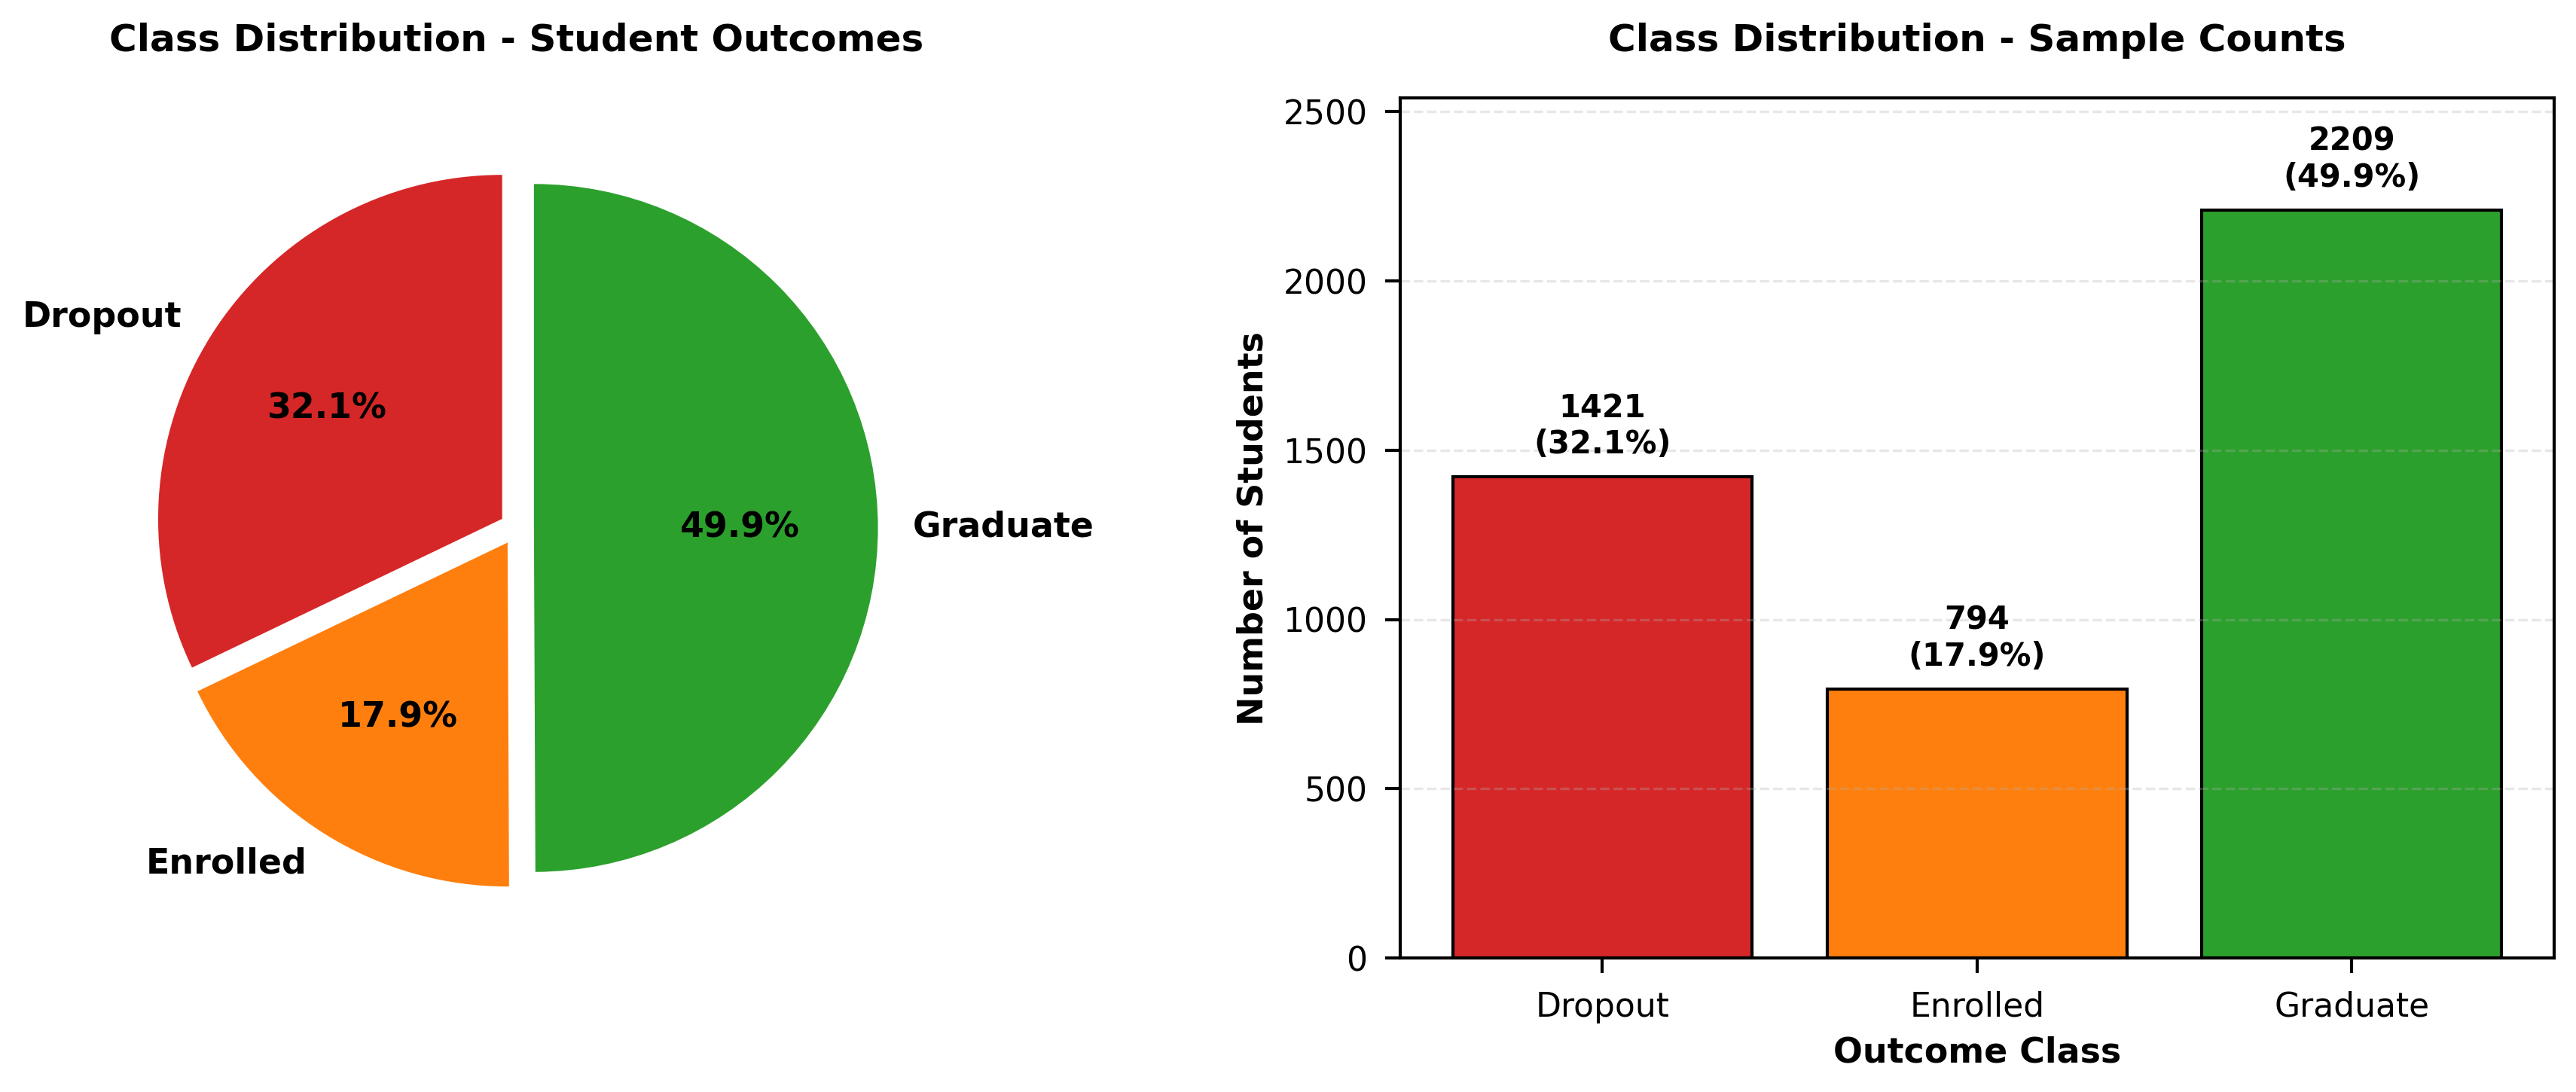
\includegraphics[width=0.7\textwidth]{supervisor_requirements/outputs/figures/01_class_distribution.png}
    \caption{Distribution of student outcomes across three classes}
    \label{fig:class_distribution}
\end{figure}

\subsection{Feature Distribution Across Domains}

\begin{table}[htbp]
\centering
\caption{Feature distribution across different domains}
\label{tab:feature_distribution}
\begin{tabular}{lcc}
\hline
\textbf{Domain} & \textbf{Number of Features} & \textbf{Percentage} \\
\hline
Academic & 18 & 52.9\% \\
Financial & 12 & 35.3\% \\
Demographic & 16 & 47.1\% \\
\hline
\textbf{Total Unique} & \textbf{34} & \textbf{100\%} \\
\hline
\end{tabular}
\end{table}

\section{Feature Analysis}
\label{sec:feature_analysis}

\subsection{Academic Features (18 features)}

\begin{enumerate}
    \item Curricular units 1st sem (credited)
    \item Curricular units 1st sem (enrolled)
    \item Curricular units 1st sem (evaluations)
    \item Curricular units 1st sem (approved)
    \item Curricular units 1st sem (grade)
    \item Curricular units 1st sem (without evaluations)
    \item Curricular units 2nd sem (credited)
    \item Curricular units 2nd sem (enrolled)
    \item Curricular units 2nd sem (evaluations)
    \item Curricular units 2nd sem (approved)
    \item Curricular units 2nd sem (grade)
    \item Curricular units 2nd sem (without evaluations)
    \item Previous qualification grade
    \item Admission grade
    \item Application mode
    \item Application order
    \item Course
    \item Daytime/evening attendance
\end{enumerate}

\subsection{Financial Features (12 features)}

\begin{enumerate}
    \item Tuition fees up to date
    \item Scholarship holder
    \item Debtor
    \item Unemployment rate
    \item Inflation rate
    \item GDP
    \item International
    \item Displaced
    \item Educational special needs
    \item Gender
    \item Age at enrollment
    \item Nationality
\end{enumerate}

\subsection{Demographic Features (16 features)}

\begin{enumerate}
    \item Marital status
    \item Previous qualification
    \item Mother's qualification
    \item Father's qualification
    \item Mother's occupation
    \item Father's occupation
    \item Gender
    \item Age at enrollment
    \item International
    \item Displaced
    \item Educational special needs
    \item Debtor
    \item Tuition fees up to date
    \item Scholarship holder
    \item Nationality
    \item Application mode
\end{enumerate}

\section{Feature Ranking Results}
\label{sec:feature_ranking}

Five complementary ranking methods were employed: Information Gain, Gain Ratio, Gini Index, Chi-Square, and ANOVA F-statistic.

\subsection{Top 20 Features}

\begin{table}[htbp]
\centering
\caption{Top 20 features ranked by average performance across all methods}
\label{tab:top20_features}
\resizebox{\textwidth}{!}{%
\begin{tabular}{clcccccccc}
\hline
\textbf{Rank} & \textbf{Feature} & \textbf{IG} & \textbf{GR} & \textbf{Gini} & \textbf{Chi2} & \textbf{F} & \textbf{Avg} \\
\hline
1 & Curricular units 2nd sem (approved) & 1 & 2 & 1 & 4 & 1 & 1.80 \\
2 & Tuition fees up to date & 6 & 1 & 2 & 7 & 5 & 4.20 \\
3 & Curricular units 2nd sem (grade) & 2 & 7 & 8 & 3 & 2 & 4.40 \\
4 & Curricular units 1st sem (approved) & 3 & 3 & 7 & 8 & 3 & 4.80 \\
5 & Curricular units 1st sem (grade) & 4 & 9 & 13 & 6 & 4 & 7.20 \\
6 & Curricular units 2nd sem (evaluations) & 5 & 10 & 5 & 15 & 11 & 9.20 \\
7 & Scholarship holder & 10 & 5 & 24 & 1 & 6 & 9.20 \\
8 & Age at enrollment & 11 & 17 & 4 & 10 & 7 & 9.80 \\
9 & Debtor & 14 & 6 & 23 & 2 & 8 & 10.60 \\
10 & Application mode & 8 & 12 & 20 & 9 & 10 & 11.80 \\
11 & Curricular units 1st sem (enrolled) & 12 & 15 & 3 & 21 & 13 & 12.80 \\
12 & Gender & 17 & 11 & 22 & 5 & 9 & 12.80 \\
13 & Curricular units 1st sem (evaluations) & 7 & 14 & 10 & 23 & 14 & 13.60 \\
14 & Curricular units 2nd sem (enrolled) & 18 & 19 & 6 & 20 & 12 & 15.00 \\
15 & Previous qualification & 16 & 13 & 27 & 12 & 20 & 17.60 \\
16 & Mother's occupation & 15 & 21 & 9 & 27 & 22 & 18.80 \\
17 & Mother's qualification & 19 & 22 & 14 & 19 & 24 & 19.60 \\
18 & Curricular units 1st sem (without evaluations) & 20 & 8 & 31 & 17 & 23 & 19.80 \\
19 & Displaced & 24 & 25 & 26 & 11 & 15 & 20.20 \\
20 & Father's occupation & 21 & 26 & 12 & 25 & 17 & 20.20 \\
\hline
\end{tabular}%
}
\end{table}

\begin{figure}[htbp]
    \centering
    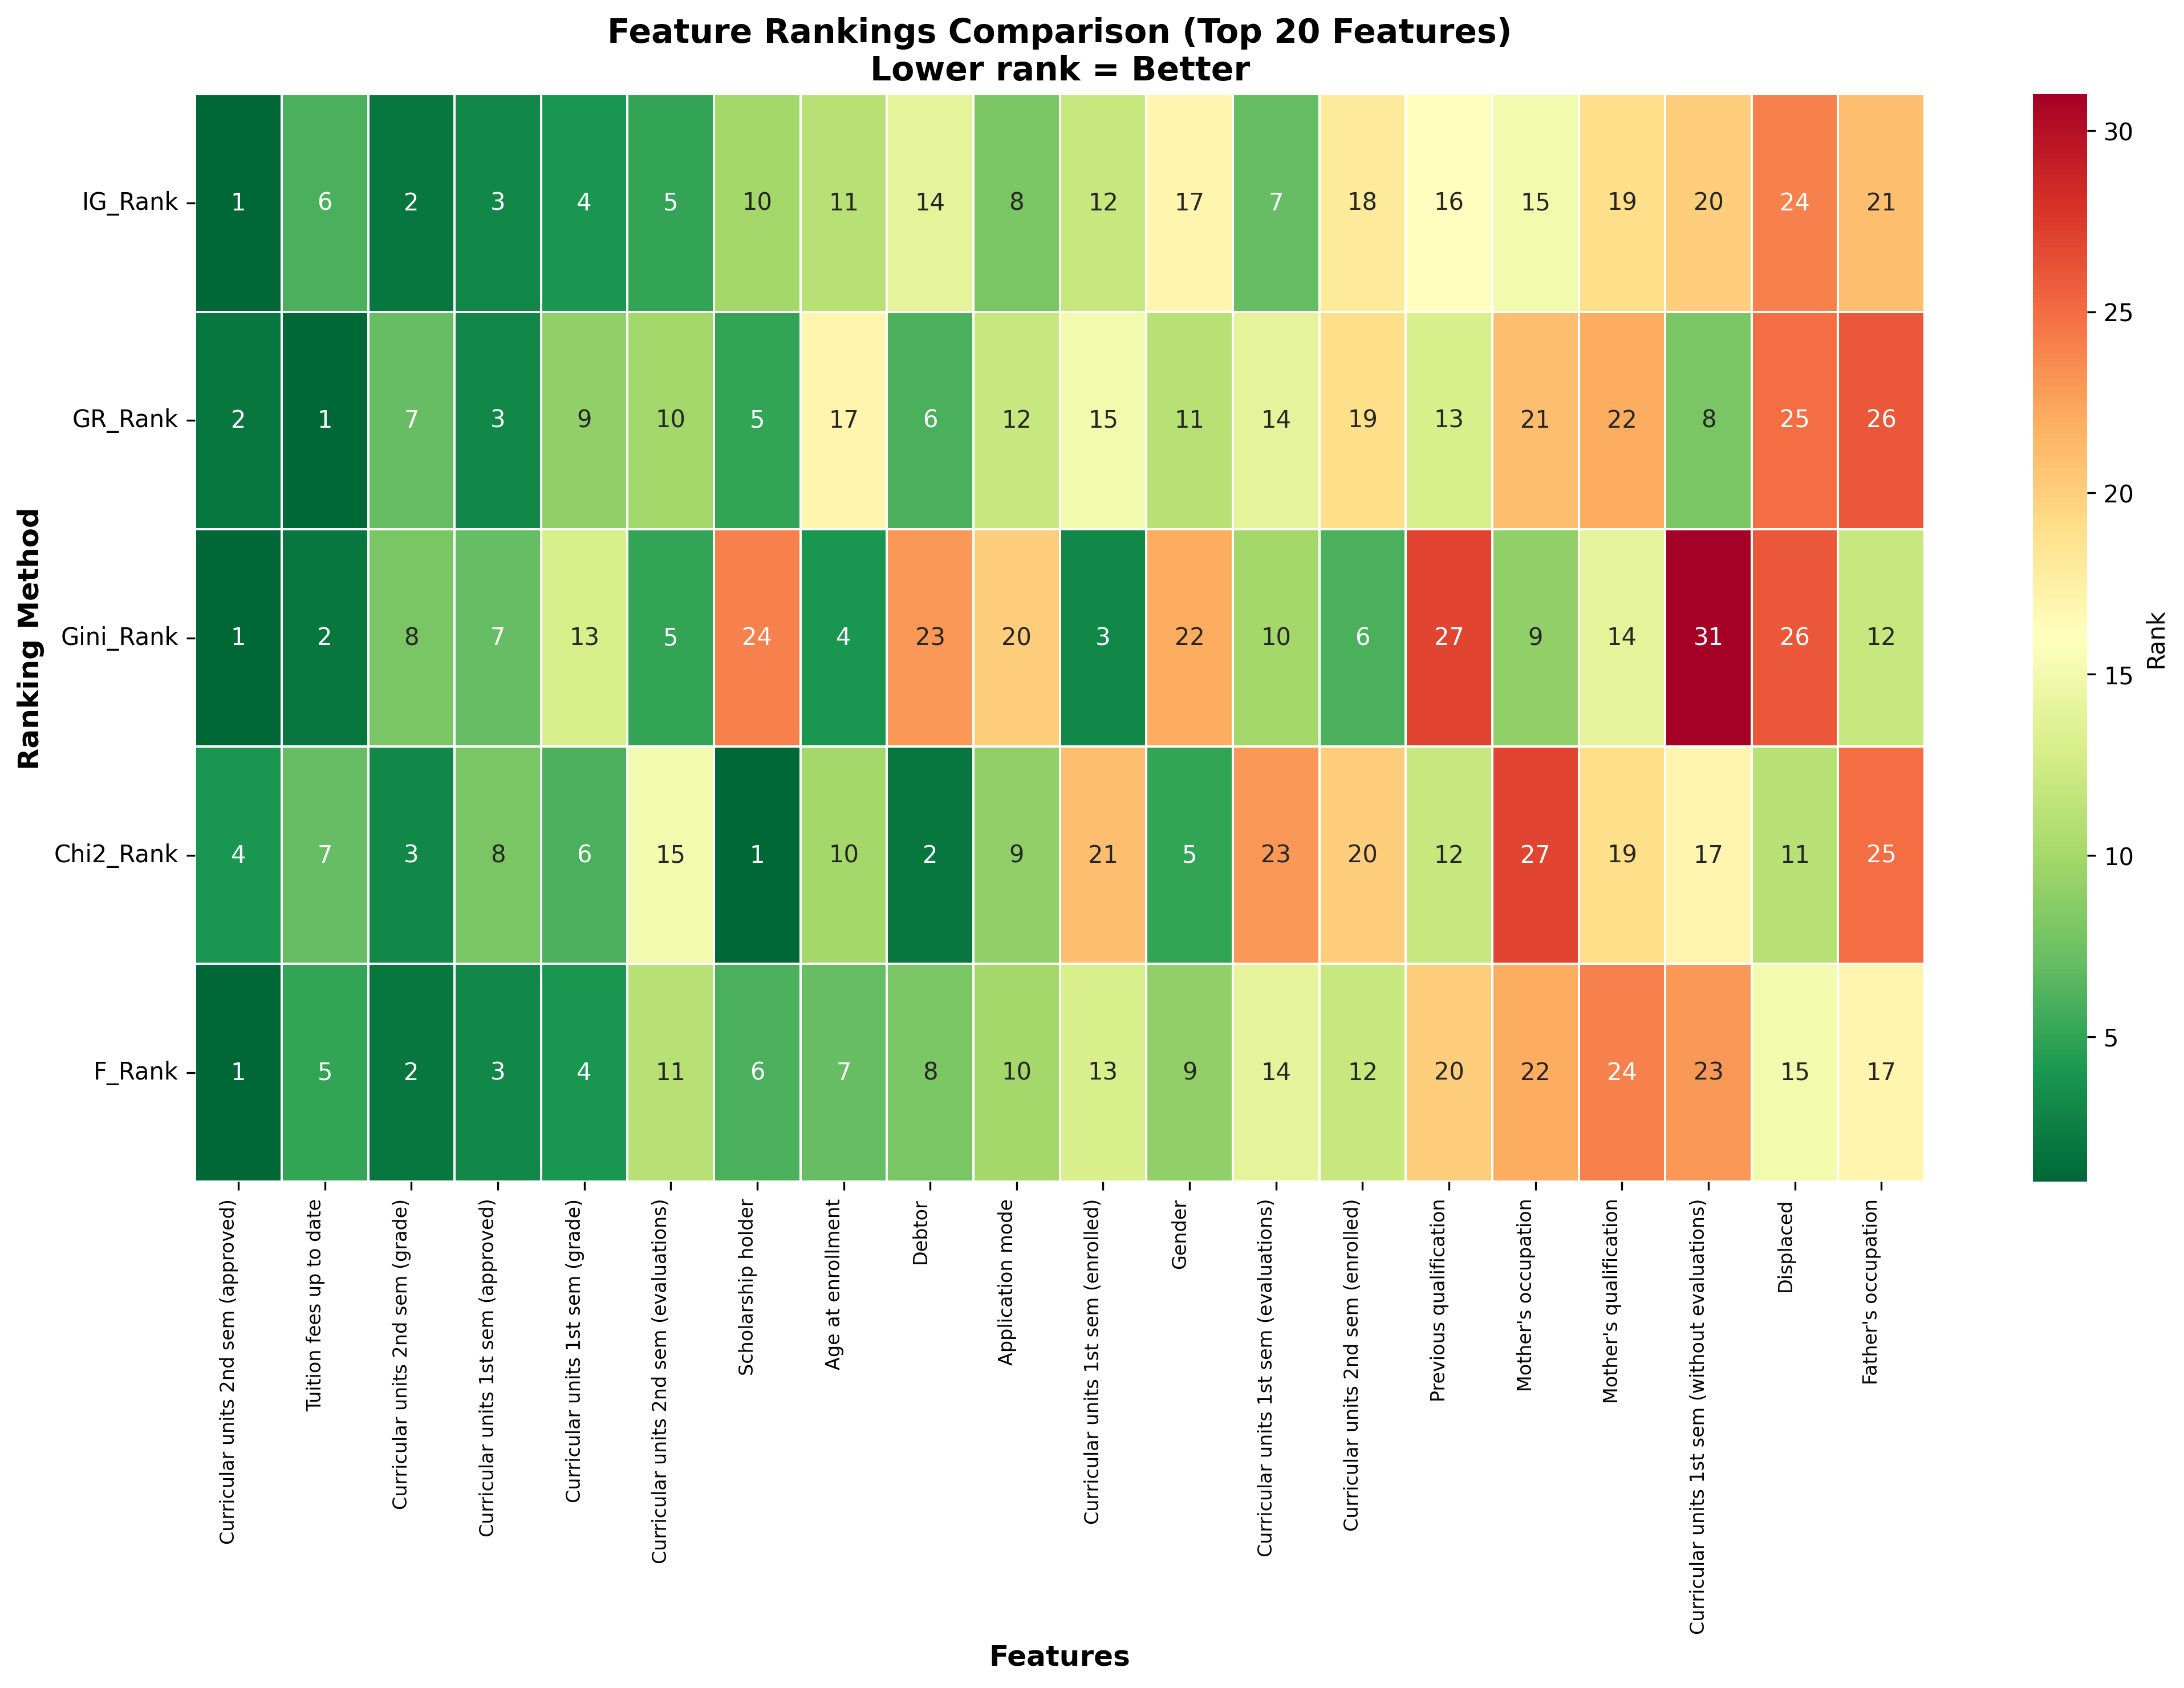
\includegraphics[width=0.85\textwidth]{supervisor_requirements/outputs/figures/03_ranking_heatmap.png}
    \caption{Heatmap visualization of feature rankings across different methods}
    \label{fig:ranking_heatmap}
\end{figure}

\subsection{Most Important Features for Dropout Prediction}

\textbf{Top-Tier Features (Average Rank < 5.0)}:
\begin{enumerate}
    \item \textbf{Curricular units 2nd sem (approved)} (Rank: 1.80)
    \item \textbf{Tuition fees up to date} (Rank: 4.20)
    \item \textbf{Curricular units 2nd sem (grade)} (Rank: 4.40)
    \item \textbf{Curricular units 1st sem (approved)} (Rank: 4.80)
\end{enumerate}

\begin{figure}[htbp]
    \centering
    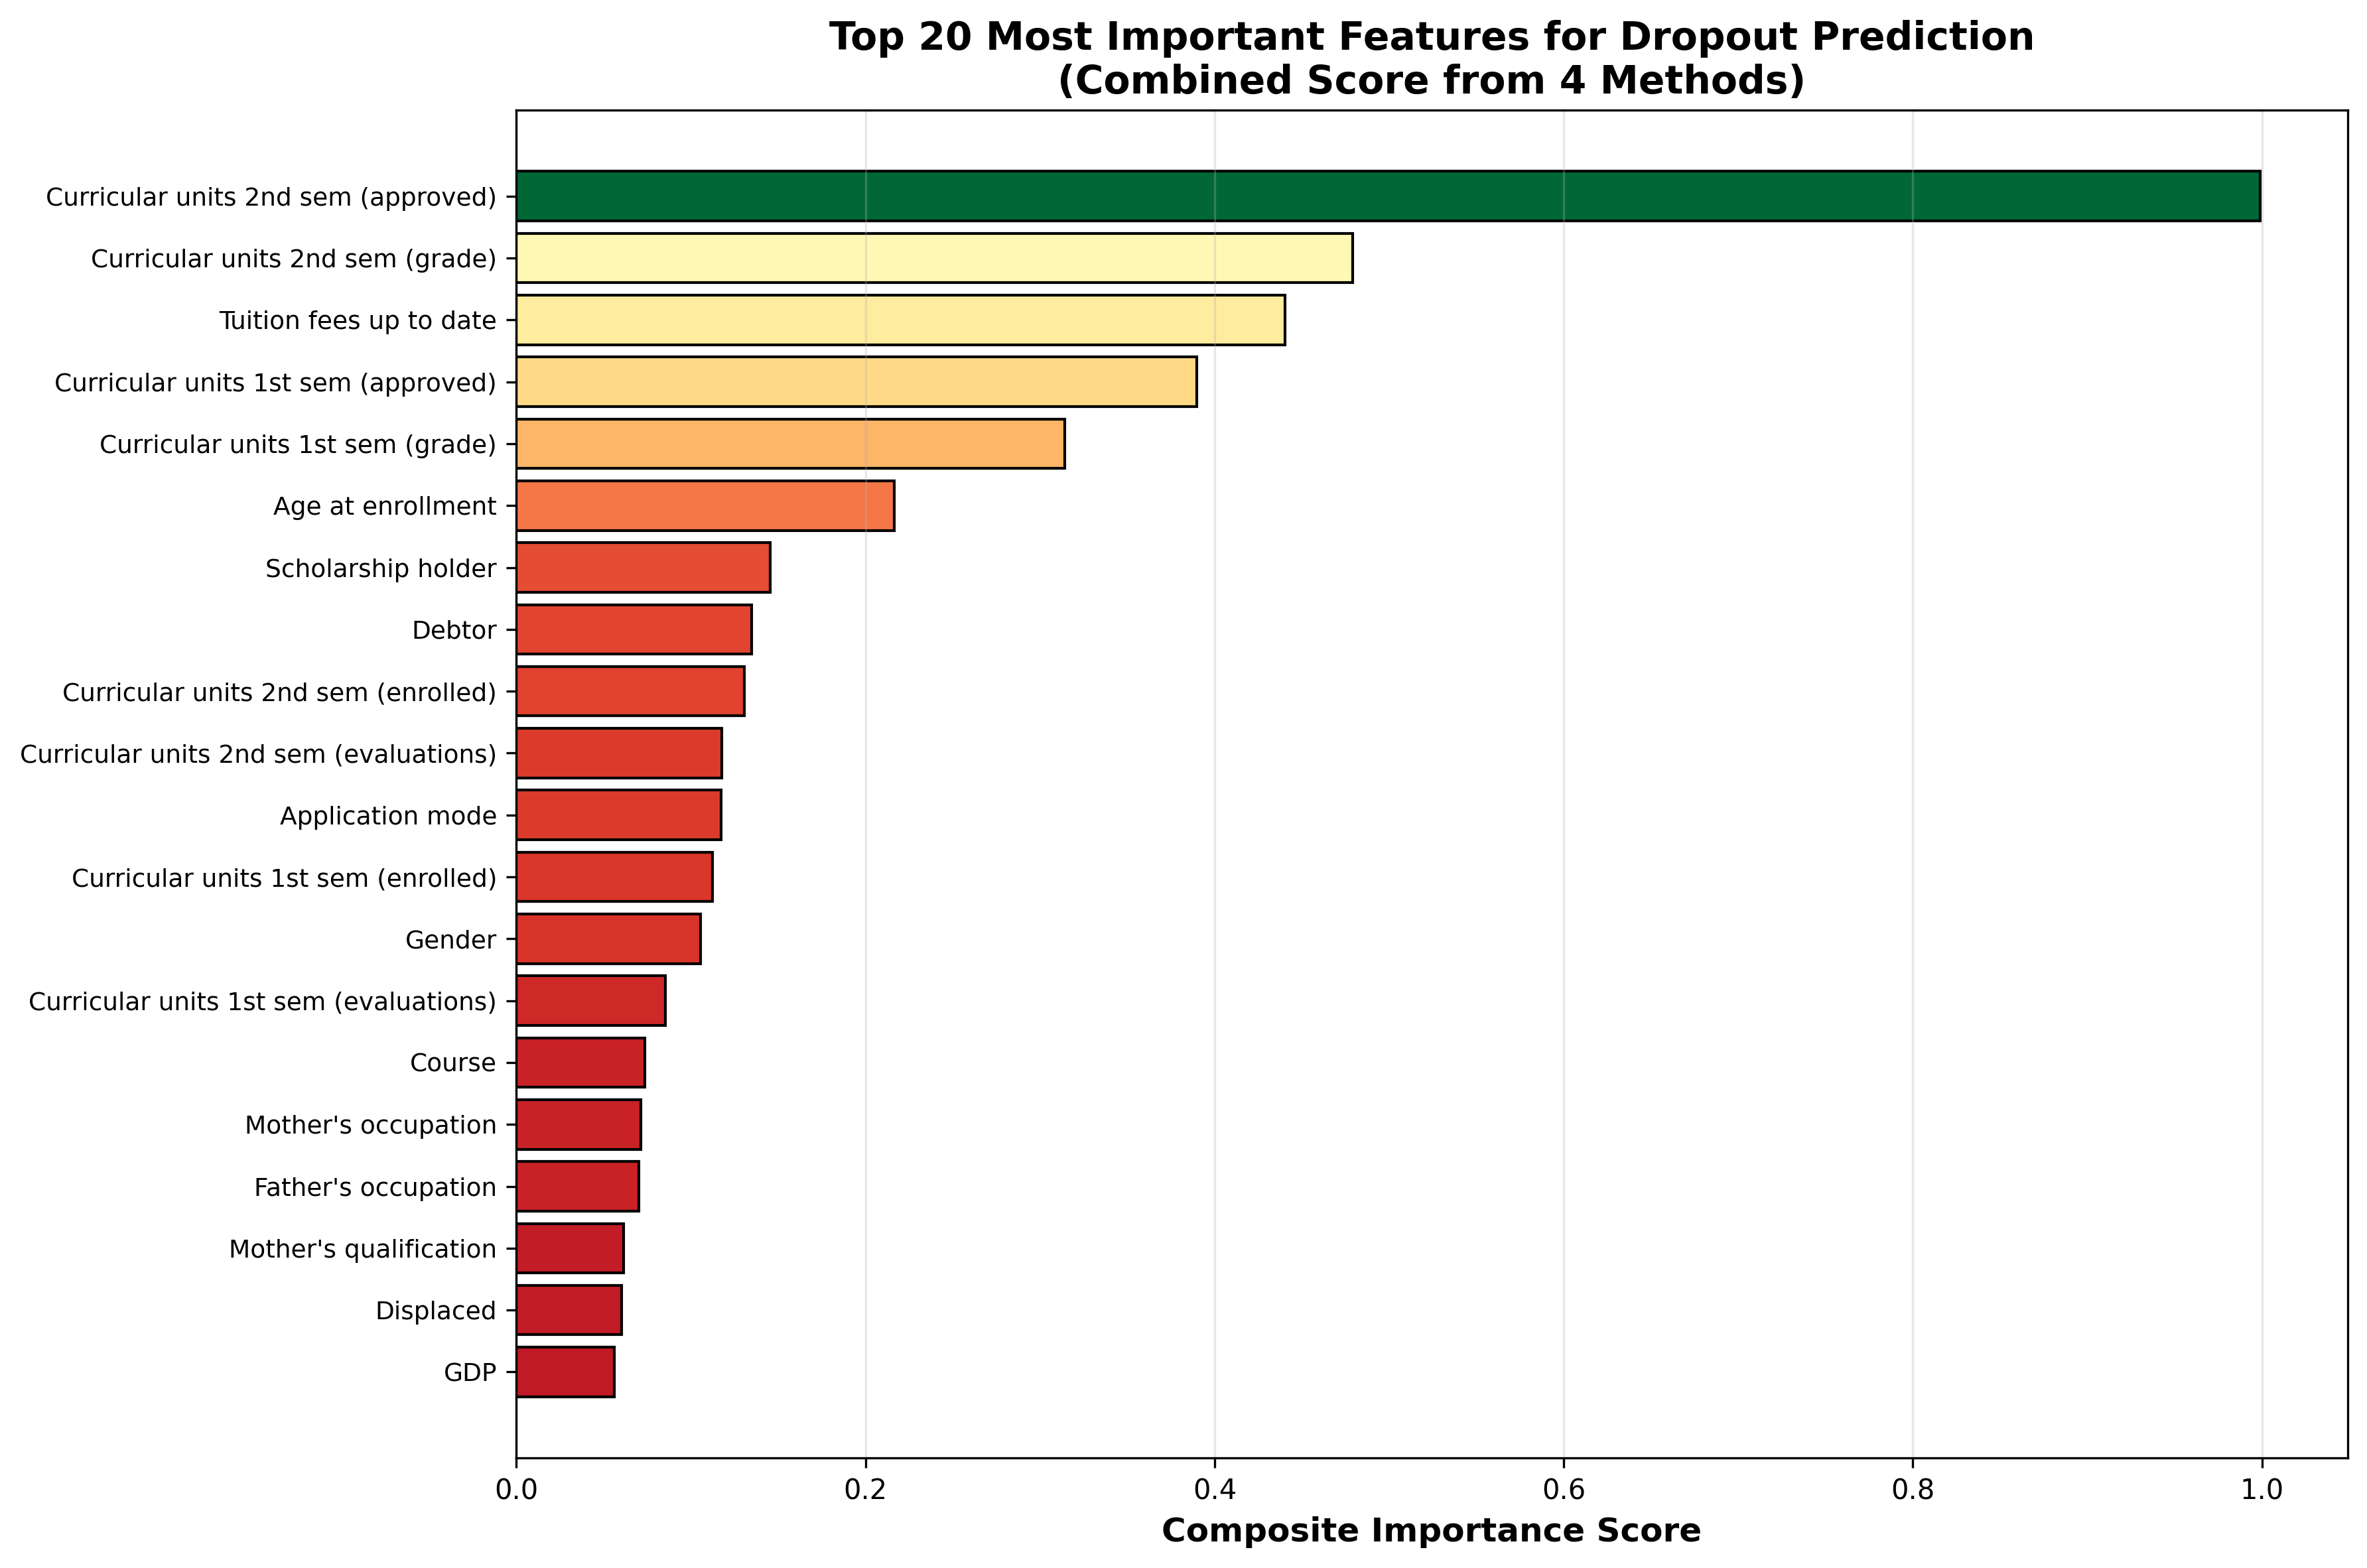
\includegraphics[width=0.8\textwidth]{supervisor_requirements/outputs/figures/04_top20_dropout_features.png}
    \caption{Top 20 most important features for dropout prediction}
    \label{fig:top20_dropout}
\end{figure}

\begin{figure}[htbp]
    \centering
    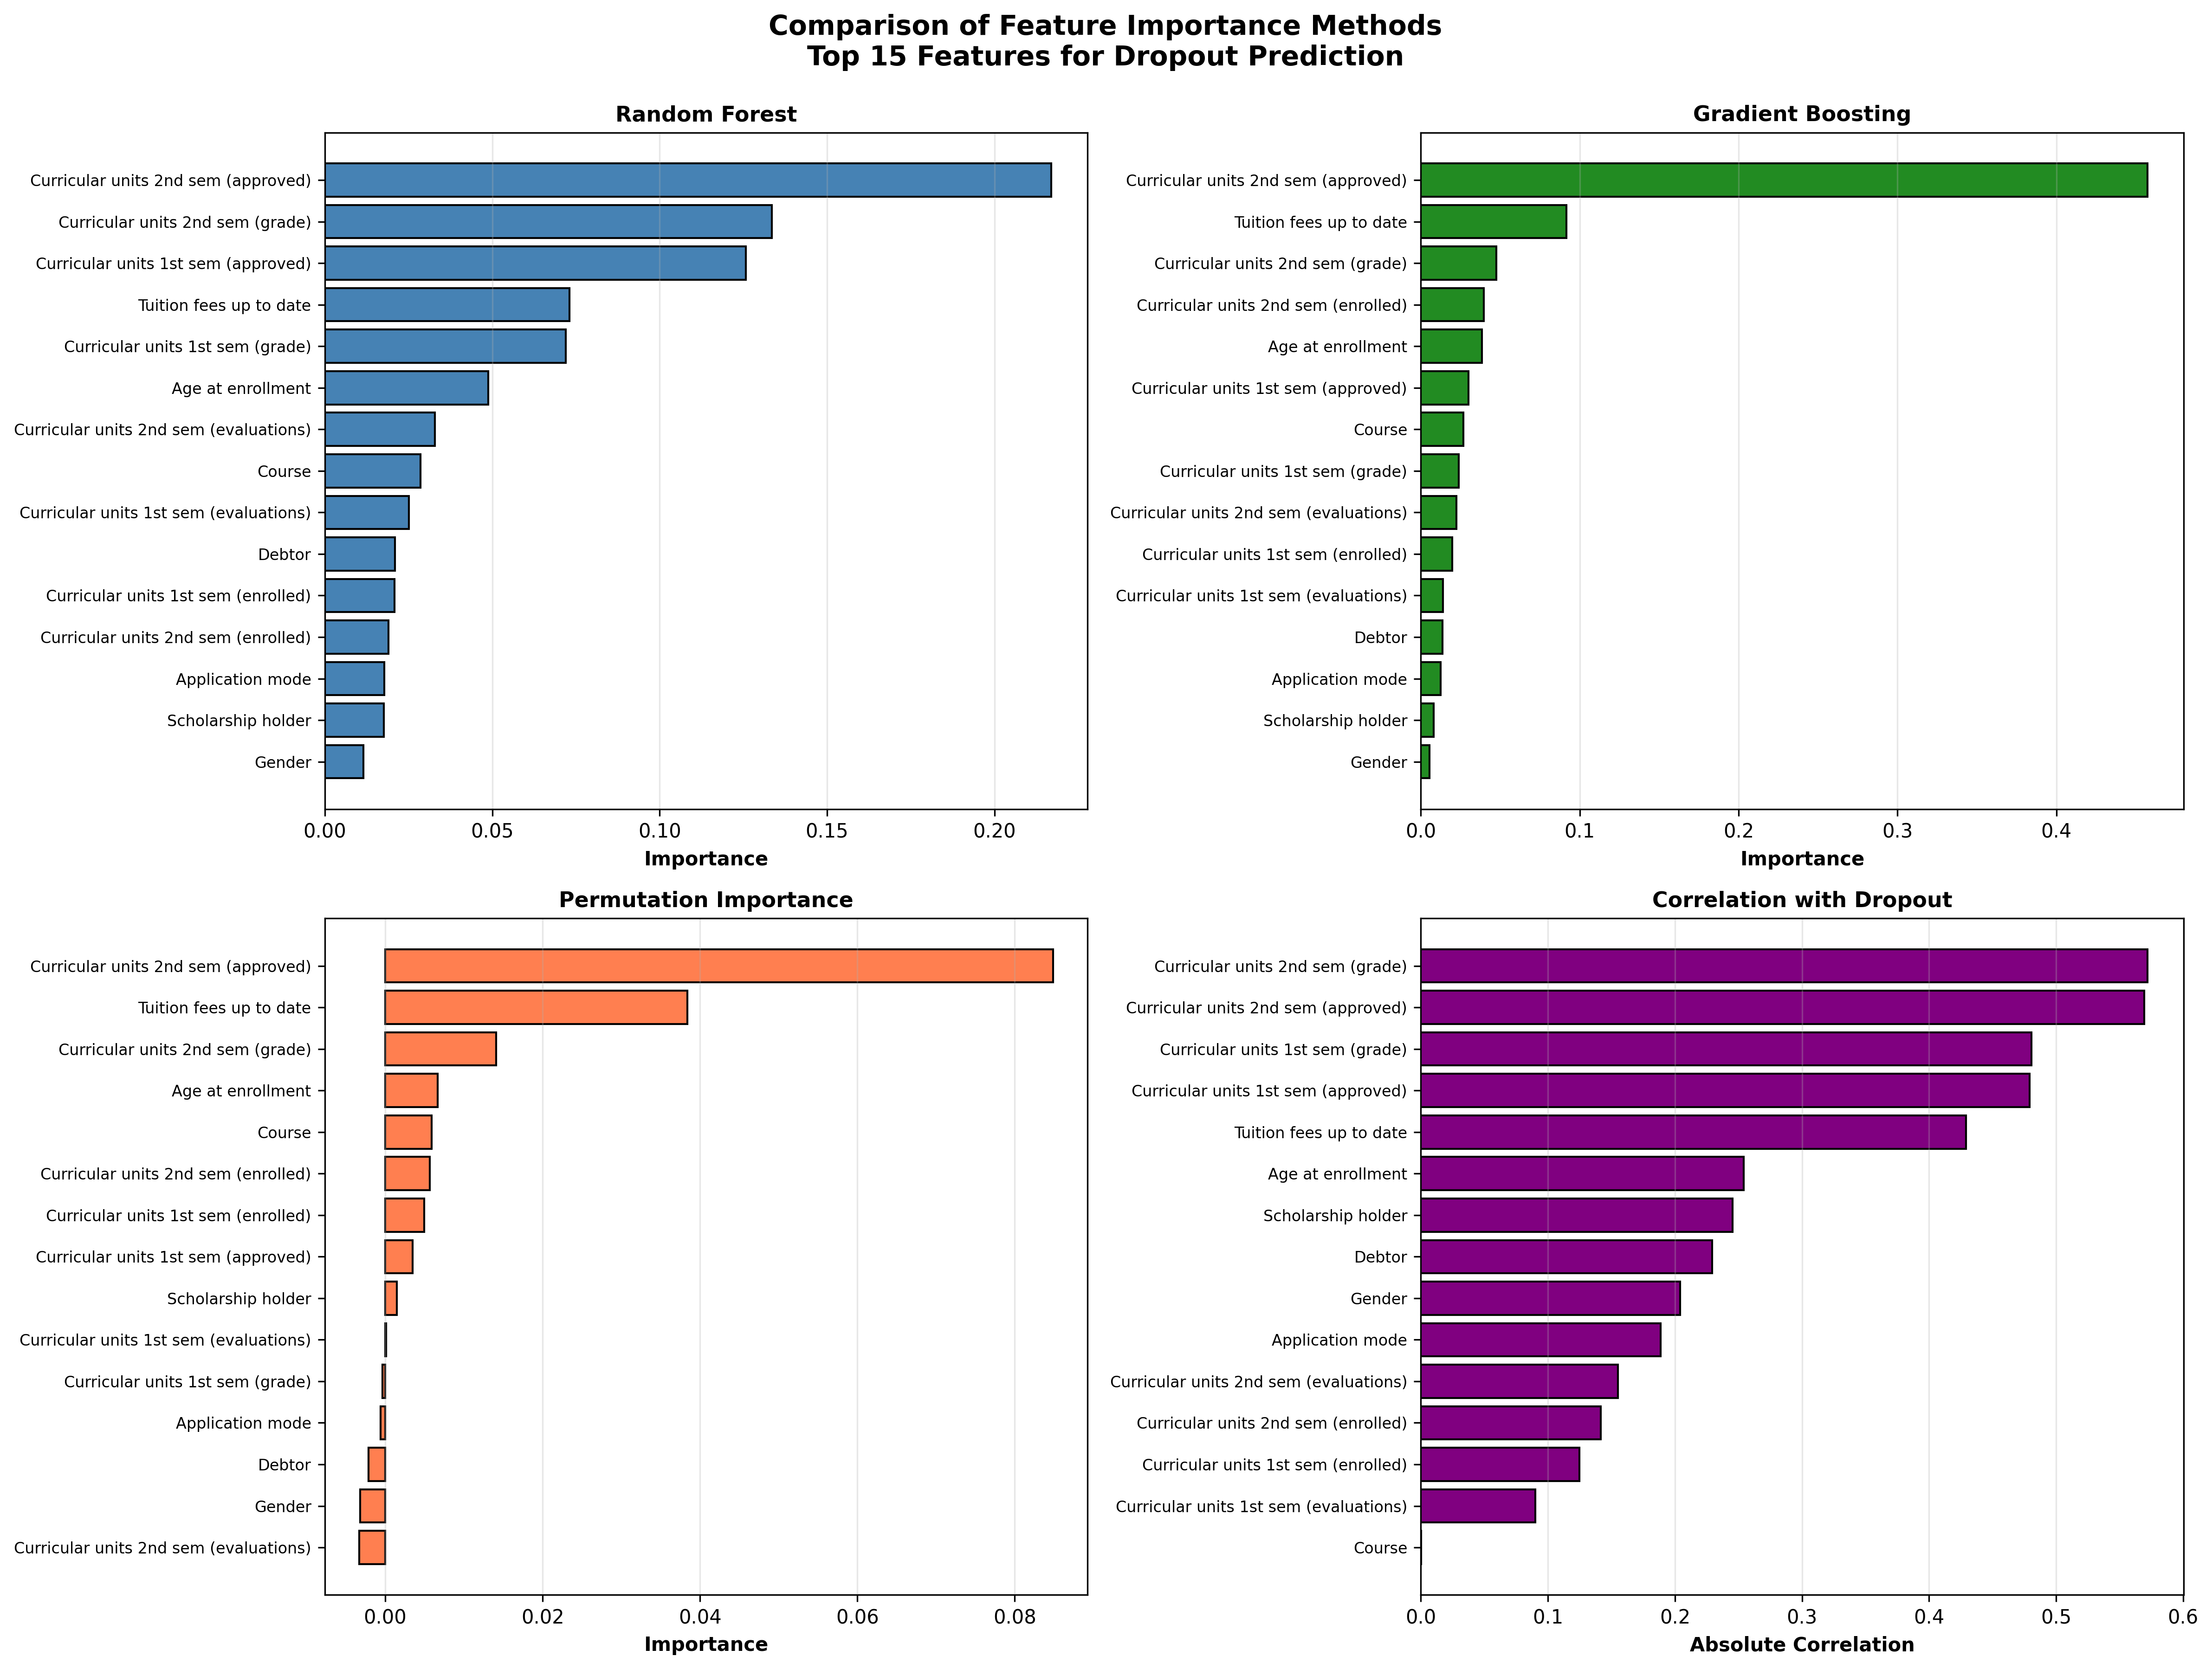
\includegraphics[width=0.85\textwidth]{supervisor_requirements/outputs/figures/04_methods_comparison.png}
    \caption{Comparison of top features across different ranking methods}
    \label{fig:methods_comparison}
\end{figure}

\section{Baseline Model Performance}
\label{sec:baseline_models}

Six machine learning models representing diverse algorithmic approaches were evaluated.

\subsection{Model Categories}

\textbf{Single Classifiers}:
\begin{itemize}
    \item Decision Tree
    \item Naive Bayes
\end{itemize}

\textbf{Ensemble Methods}:
\begin{itemize}
    \item Random Forest (200 trees)
    \item AdaBoost (100 estimators)
    \item XGBoost (200 estimators)
\end{itemize}

\textbf{Deep Learning}:
\begin{itemize}
    \item Neural Network (3 layers: 128-64-32 neurons)
\end{itemize}

\subsection{Training vs Test Performance}

\begin{table}[htbp]
\centering
\caption{Training and test accuracy of baseline models (80/20 split: 3,539 training, 885 test)}
\label{tab:baseline_performance}
\begin{tabular}{lccc}
\hline
\textbf{Model} & \textbf{Training Acc} & \textbf{Test Acc} & \textbf{Overfit Gap} \\
\hline
Decision Tree & 85.08\% & 64.52\% & 20.56\% \\
Naive Bayes & 68.61\% & 66.67\% & 1.94\% \\
Random Forest & 88.27\% & 75.82\% & 12.45\% \\
AdaBoost & 81.60\% & 74.92\% & 6.68\% \\
XGBoost & 98.47\% & 77.40\% & 21.07\% \\
Neural Network & 89.43\% & 74.12\% & 15.31\% \\
\hline
\end{tabular}
\end{table}

\textbf{Best test performance}: XGBoost (77.40\%), followed by Random Forest (75.82\%).

\begin{figure}[htbp]
    \centering
    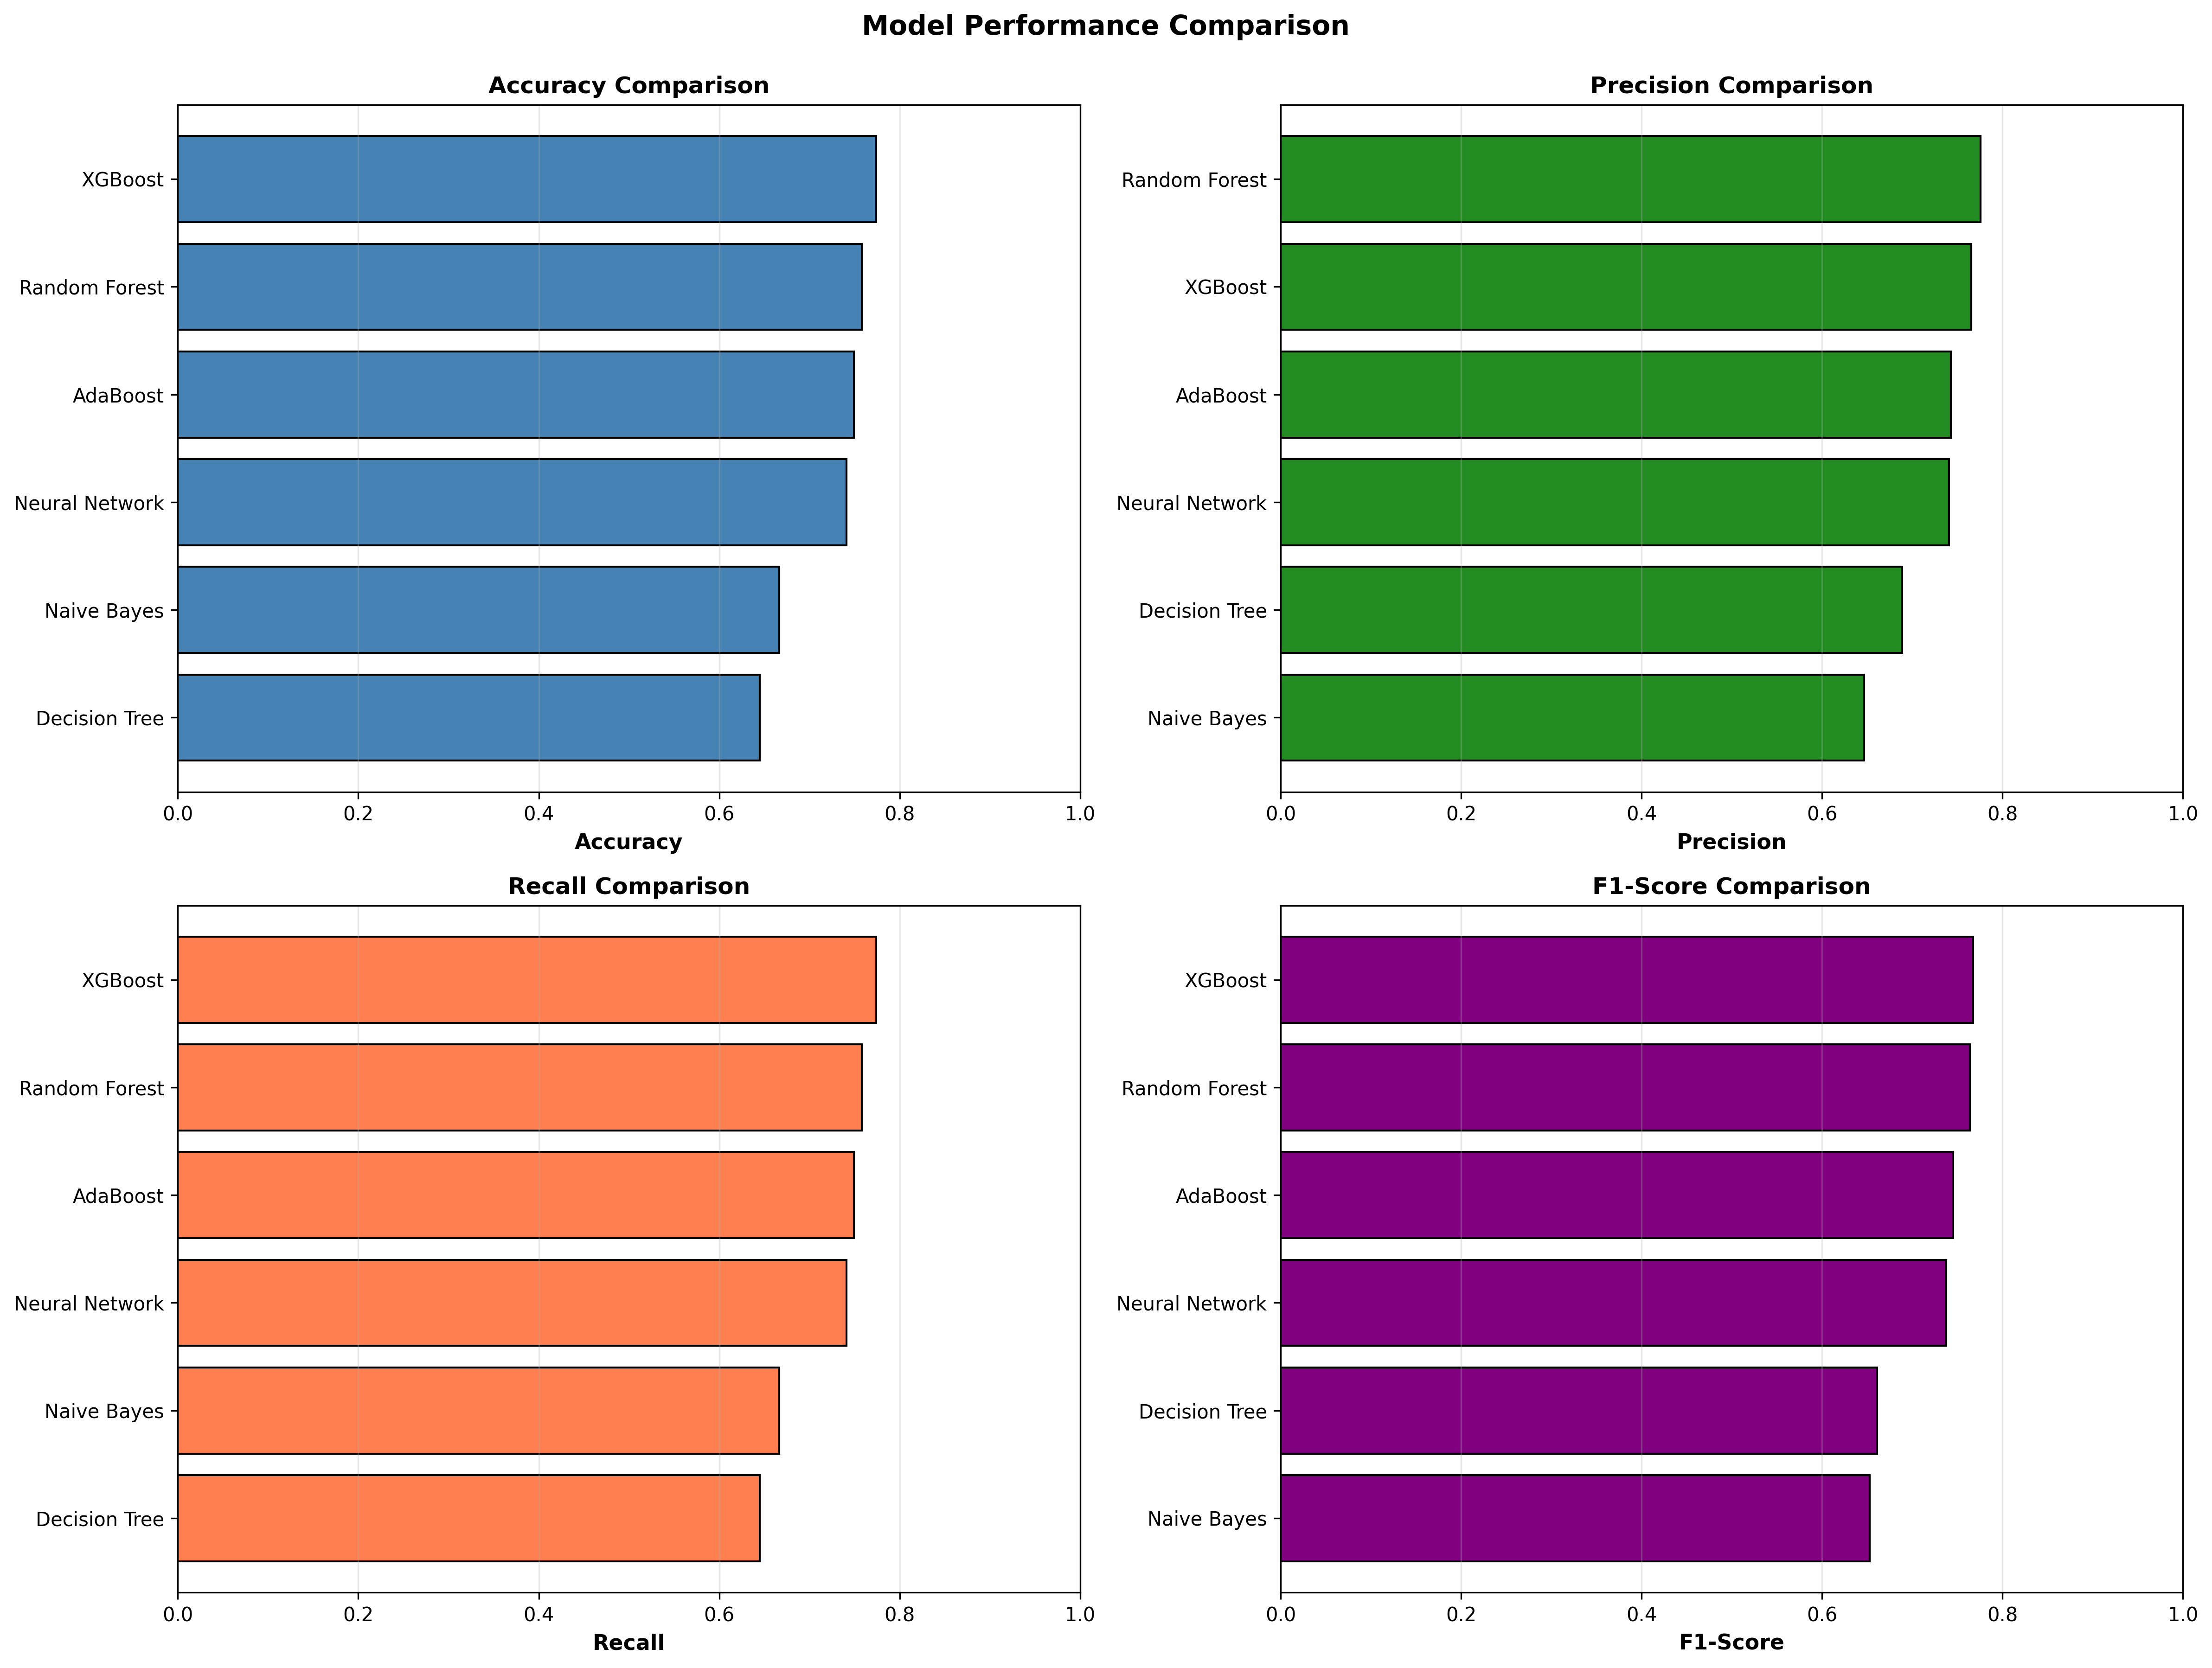
\includegraphics[width=0.8\textwidth]{supervisor_requirements/outputs/figures/07_model_comparison.png}
    \caption{Model performance comparison across training and test sets}
    \label{fig:model_comparison}
\end{figure}

\section{Detailed Model Evaluation}
\label{sec:detailed_evaluation}

\subsection{Overall Performance Metrics}

\begin{table}[htbp]
\centering
\caption{Comprehensive evaluation metrics for all models (Test Set, n=885)}
\label{tab:comprehensive_metrics}
\begin{tabular}{lccccc}
\hline
\textbf{Model} & \textbf{Accuracy} & \textbf{Precision} & \textbf{Recall} & \textbf{F1} & \textbf{AUC} \\
\hline
Decision Tree & 67.01\% & 0.6702 & 0.6701 & 0.6701 & 0.8160 \\
Naive Bayes & 70.85\% & 0.6856 & 0.7085 & 0.6848 & 0.8133 \\
Random Forest & \textbf{76.72\%} & 0.7540 & 0.7672 & 0.7561 & \textbf{0.9062} \\
AdaBoost & 74.24\% & 0.7254 & 0.7424 & 0.7308 & 0.8877 \\
XGBoost & 75.93\% & 0.7526 & 0.7593 & 0.7544 & 0.9057 \\
Neural Network & 71.41\% & 0.7064 & 0.7141 & 0.7100 & 0.8730 \\
\hline
\end{tabular}
\end{table}

\textbf{Random Forest} achieved best accuracy (76.72\%) and highest AUC (0.9062).

\begin{figure}[htbp]
    \centering
    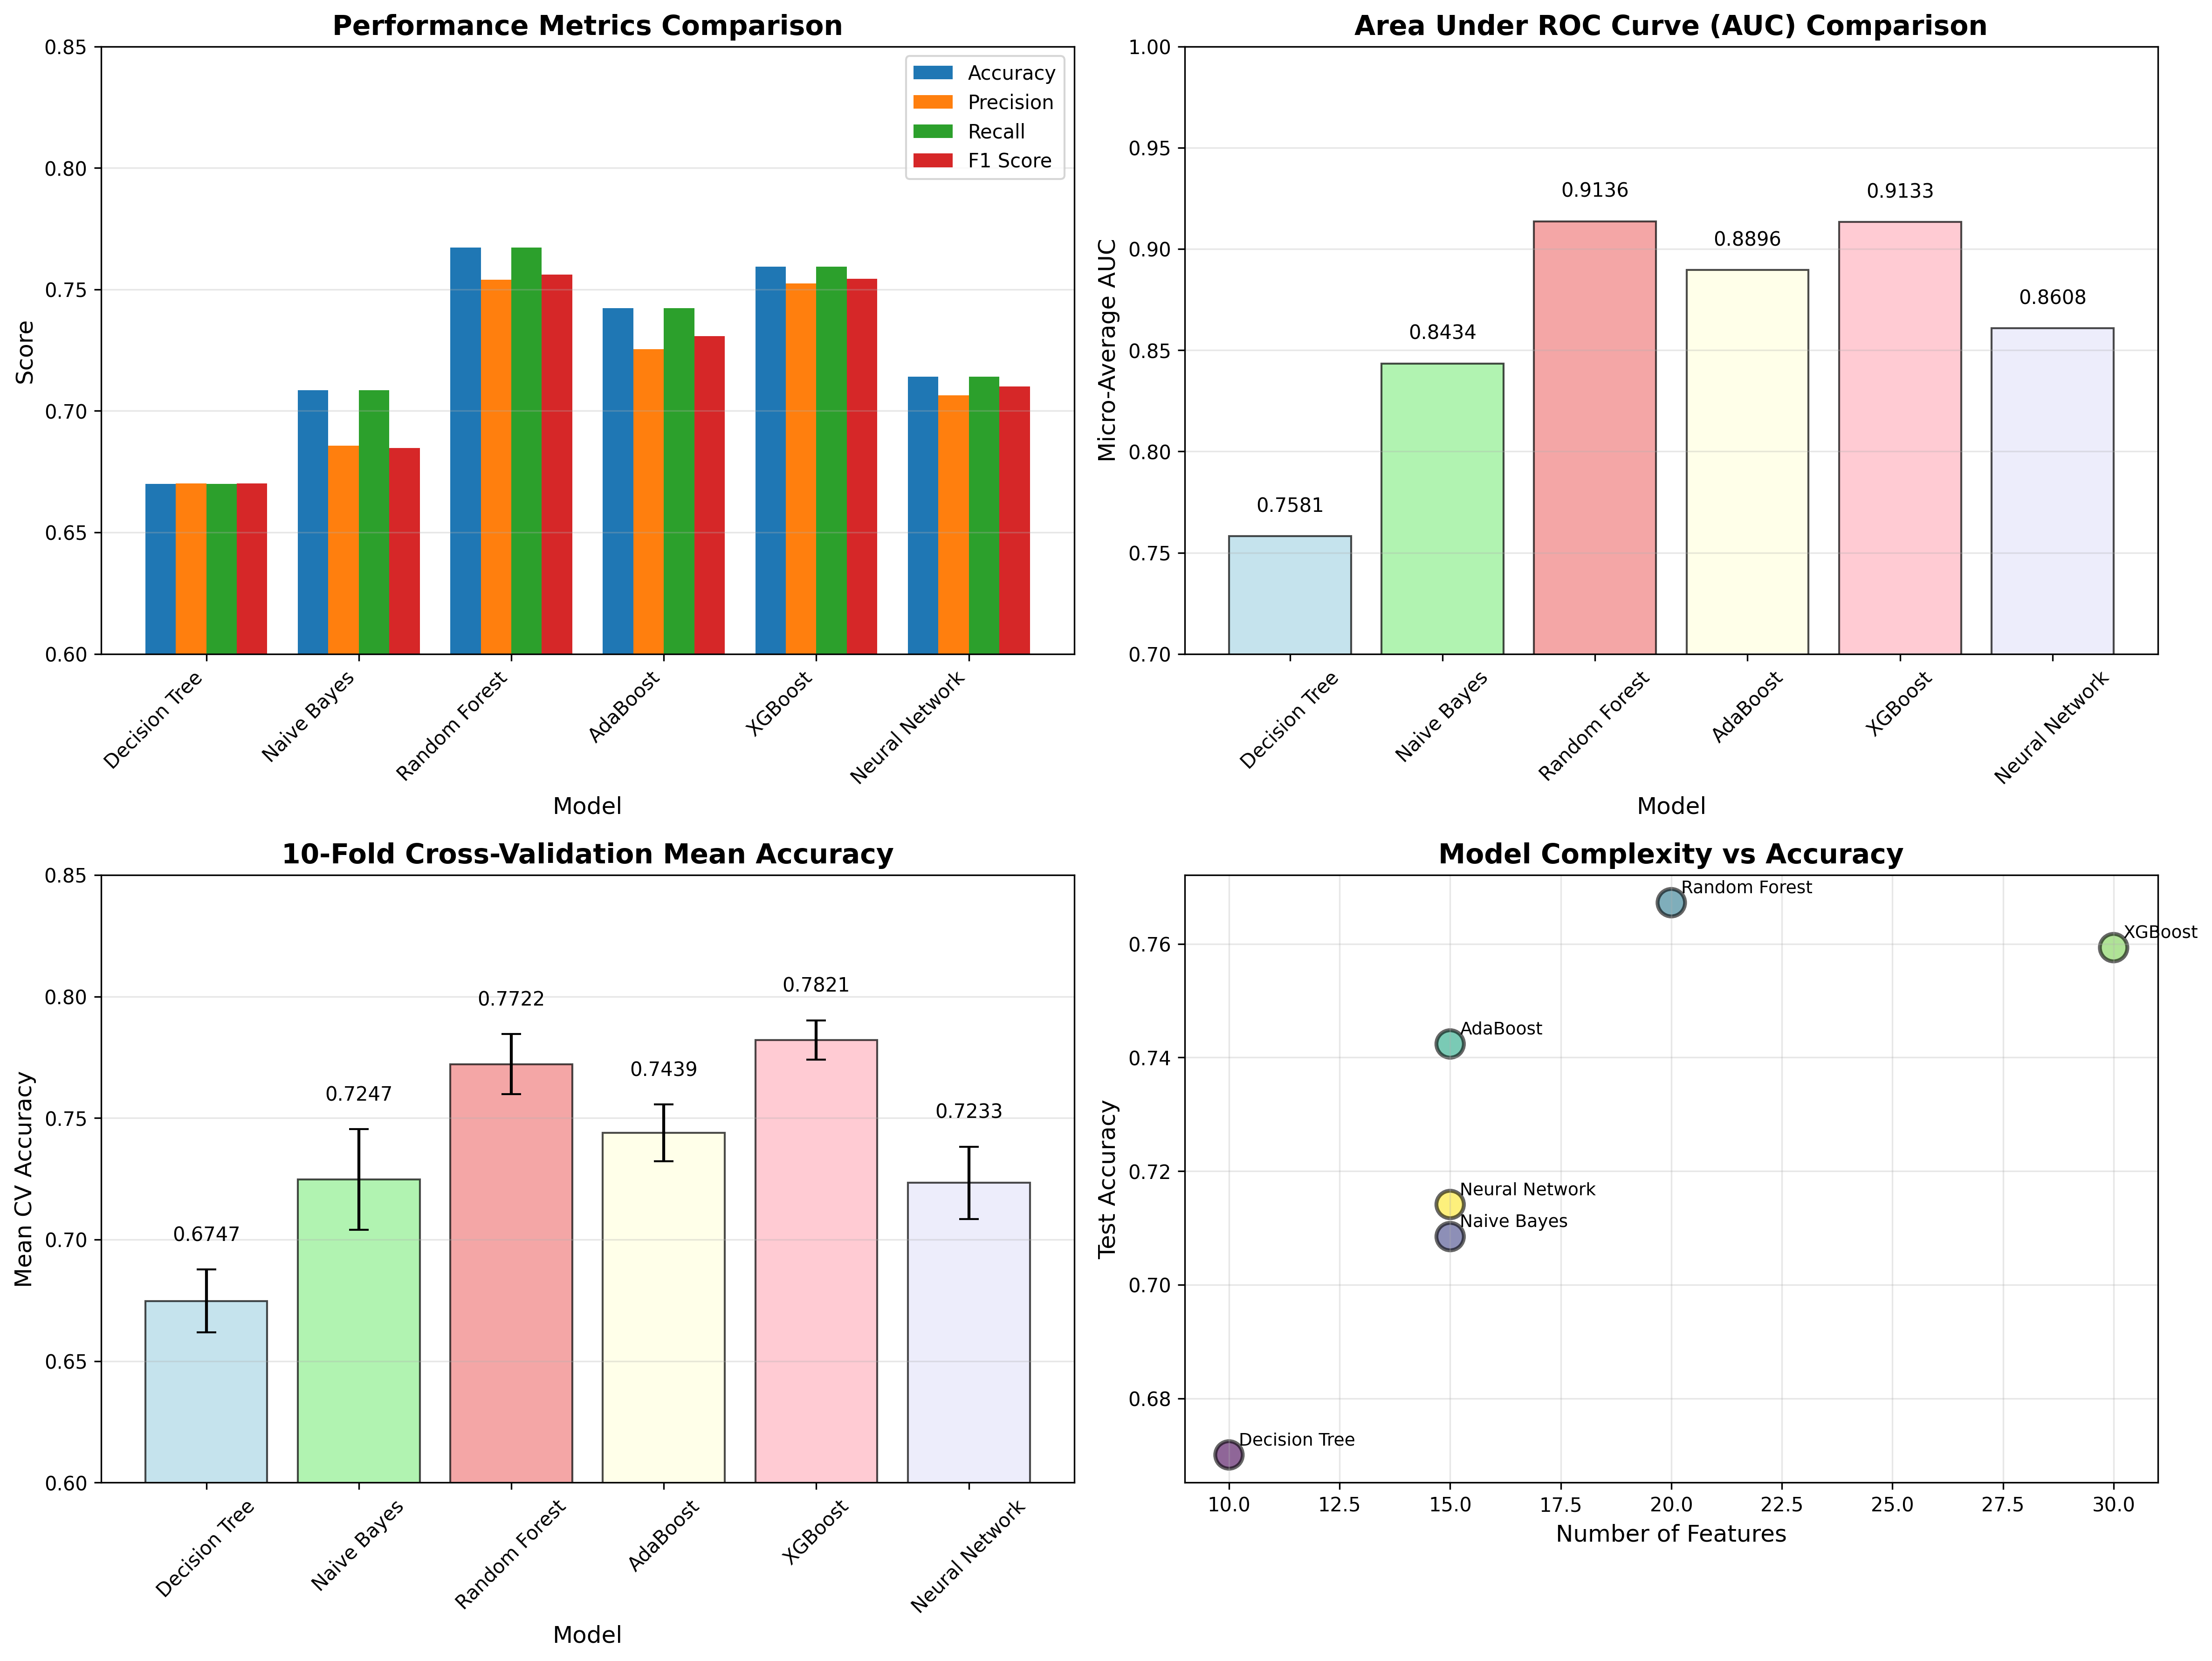
\includegraphics[width=0.85\textwidth]{supervisor_requirements/outputs/figures/12_comprehensive_metrics_comparison.png}
    \caption{Comprehensive comparison of all evaluation metrics}
    \label{fig:comprehensive_metrics}
\end{figure}

\subsection{Per-Class Performance}

\begin{table}[htbp]
\centering
\caption{Random Forest per-class performance}
\label{tab:perclass_metrics}
\begin{tabular}{lcccc}
\hline
\textbf{Class} & \textbf{Precision} & \textbf{Recall} & \textbf{F1} & \textbf{Support} \\
\hline
Dropout & 0.80 & 0.74 & 0.77 & 284 \\
Enrolled & 0.54 & 0.39 & 0.45 & 159 \\
Graduate & 0.80 & 0.92 & 0.86 & 442 \\
\hline
\textbf{Weighted Avg} & 0.75 & 0.77 & 0.76 & 885 \\
\hline
\end{tabular}
\end{table}

\begin{figure}[htbp]
    \centering
    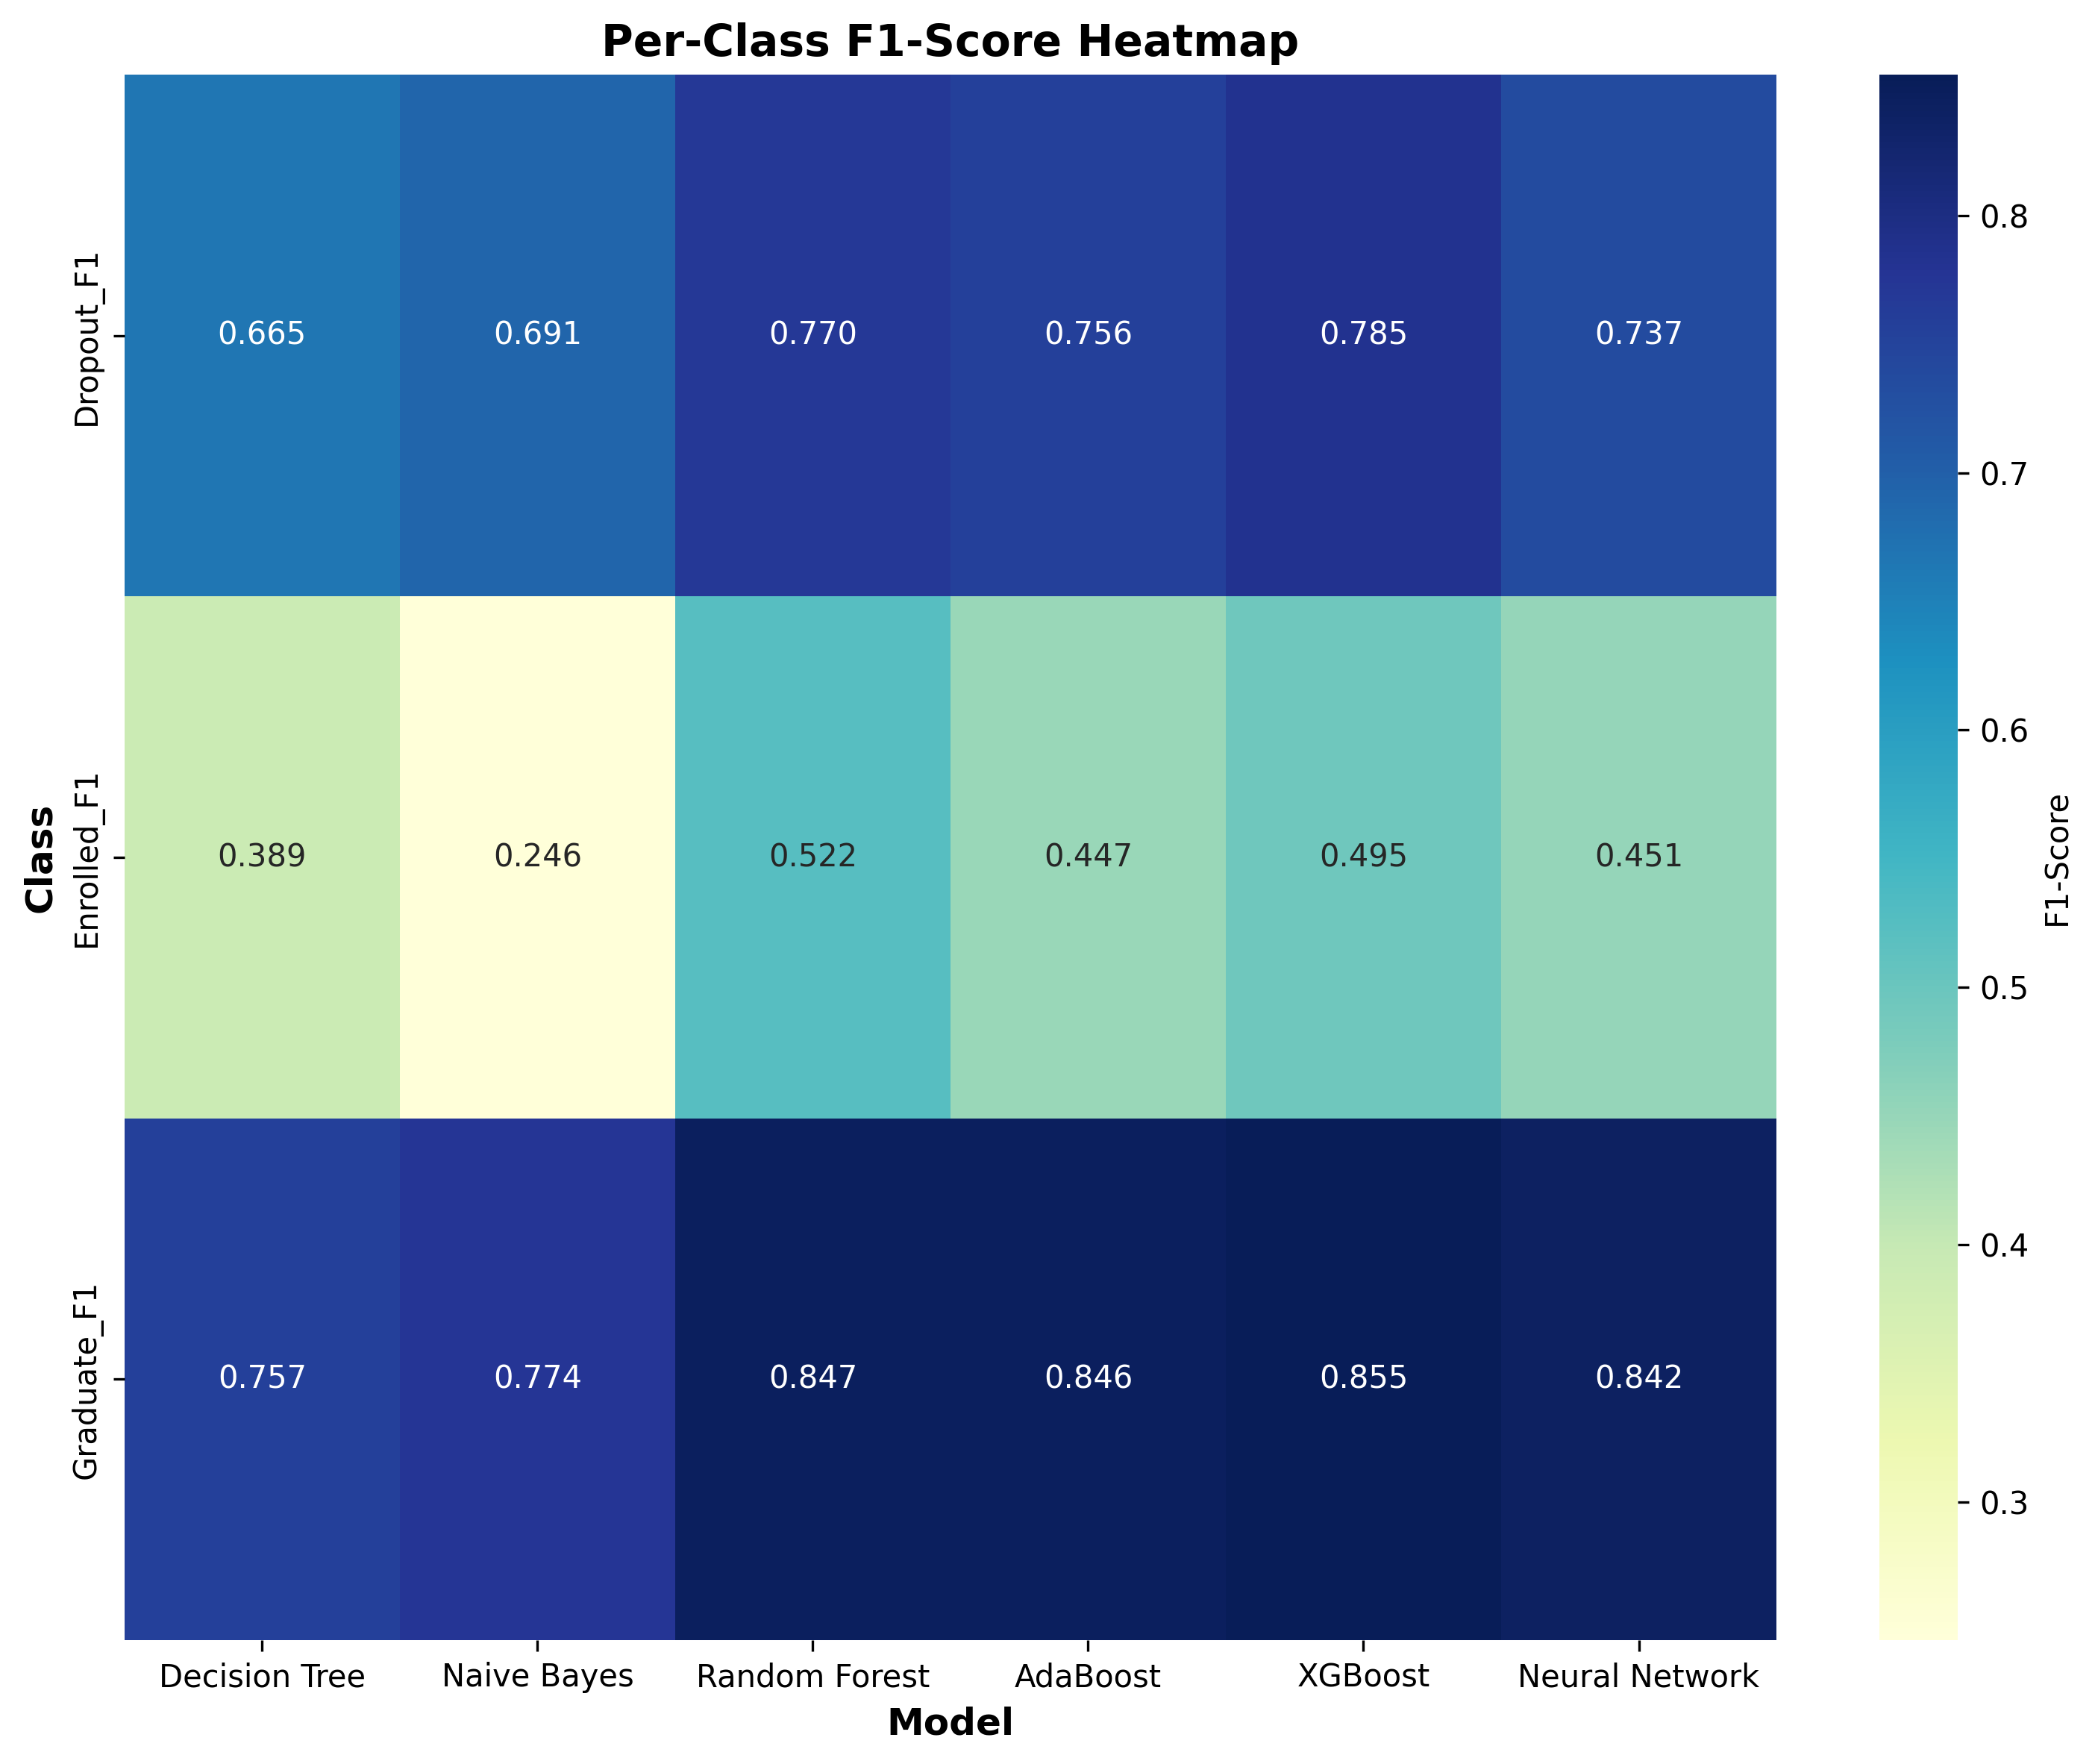
\includegraphics[width=0.8\textwidth]{supervisor_requirements/outputs/figures/07_per_class_performance.png}
    \caption{Per-class performance comparison}
    \label{fig:perclass_performance}
\end{figure}

\subsection{Confusion Matrices}

\begin{figure}[htbp]
    \centering
    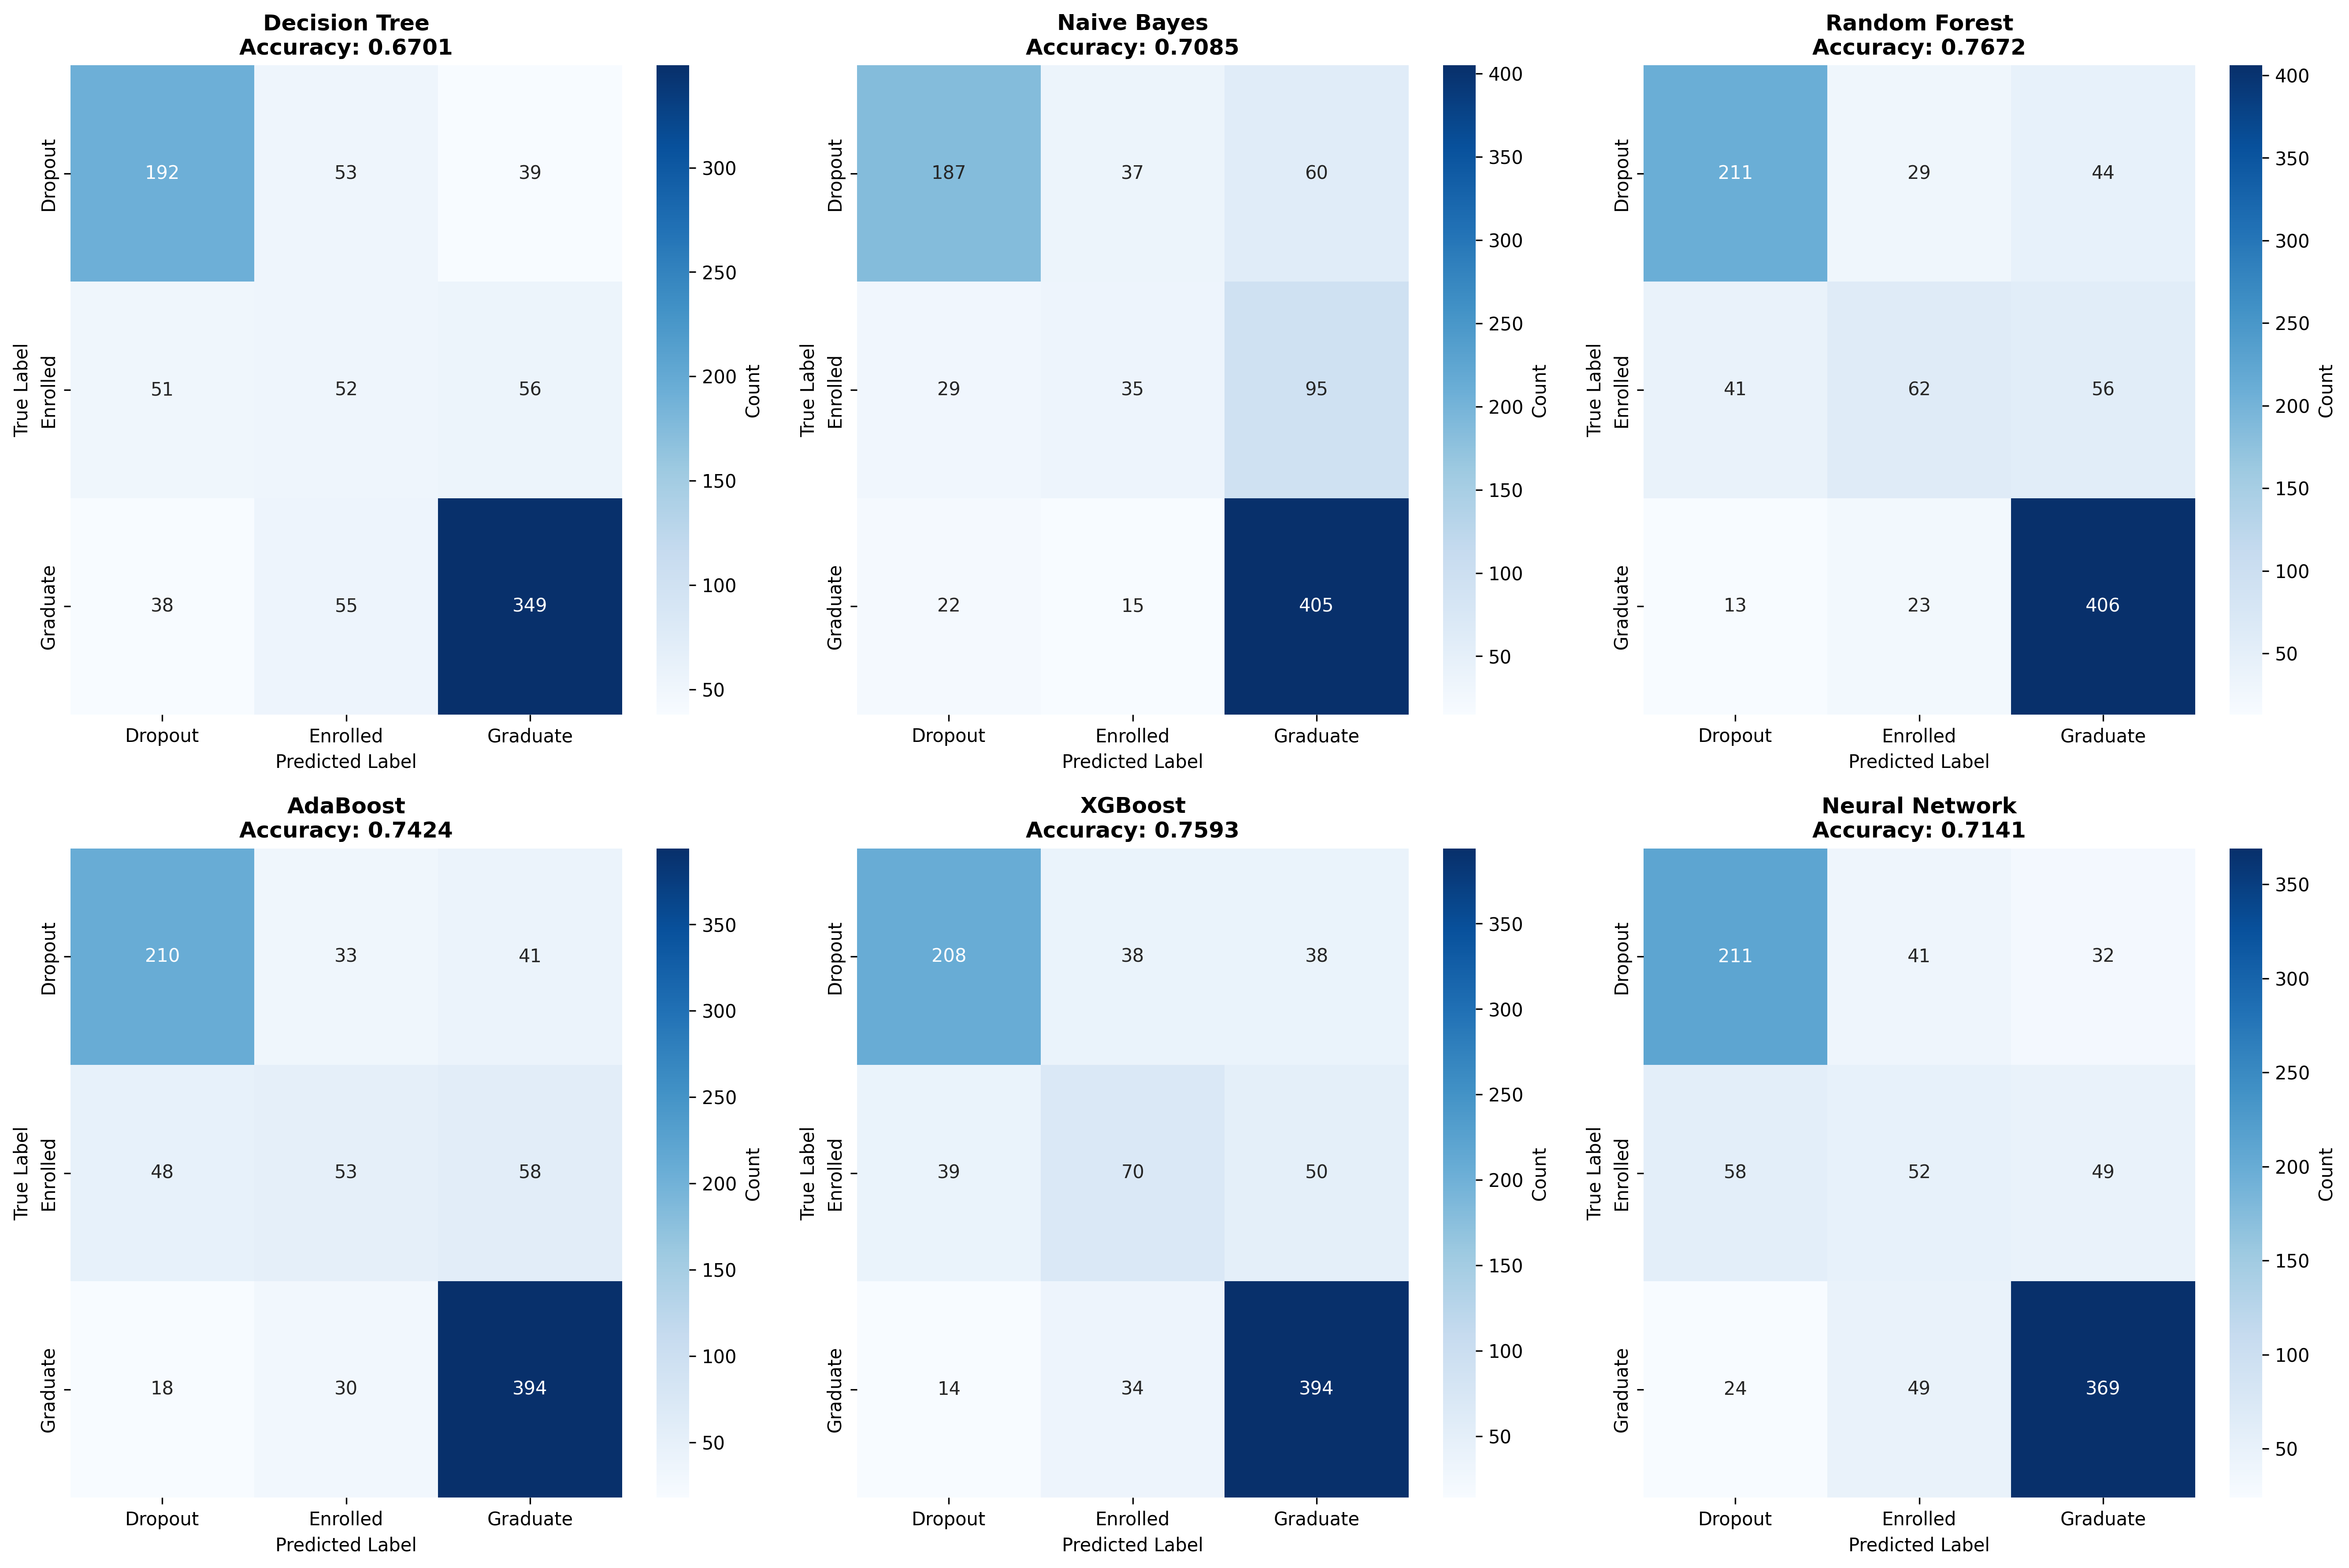
\includegraphics[width=\textwidth]{supervisor_requirements/outputs/figures/12_all_models_confusion_matrices.png}
    \caption{Confusion matrices for all six models}
    \label{fig:confusion_matrices}
\end{figure}

\begin{table}[htbp]
\centering
\caption{Random Forest confusion matrix}
\label{tab:rf_confusion}
\begin{tabular}{lccc}
\hline
\textbf{Actual/Predicted} & \textbf{Dropout} & \textbf{Enrolled} & \textbf{Graduate} \\
\hline
Dropout (284) & 211 & 29 & 44 \\
Enrolled (159) & 41 & 62 & 56 \\
Graduate (442) & 13 & 23 & 406 \\
\hline
\end{tabular}
\end{table}

\subsection{ROC Curves and AUC}

\begin{figure}[htbp]
    \centering
    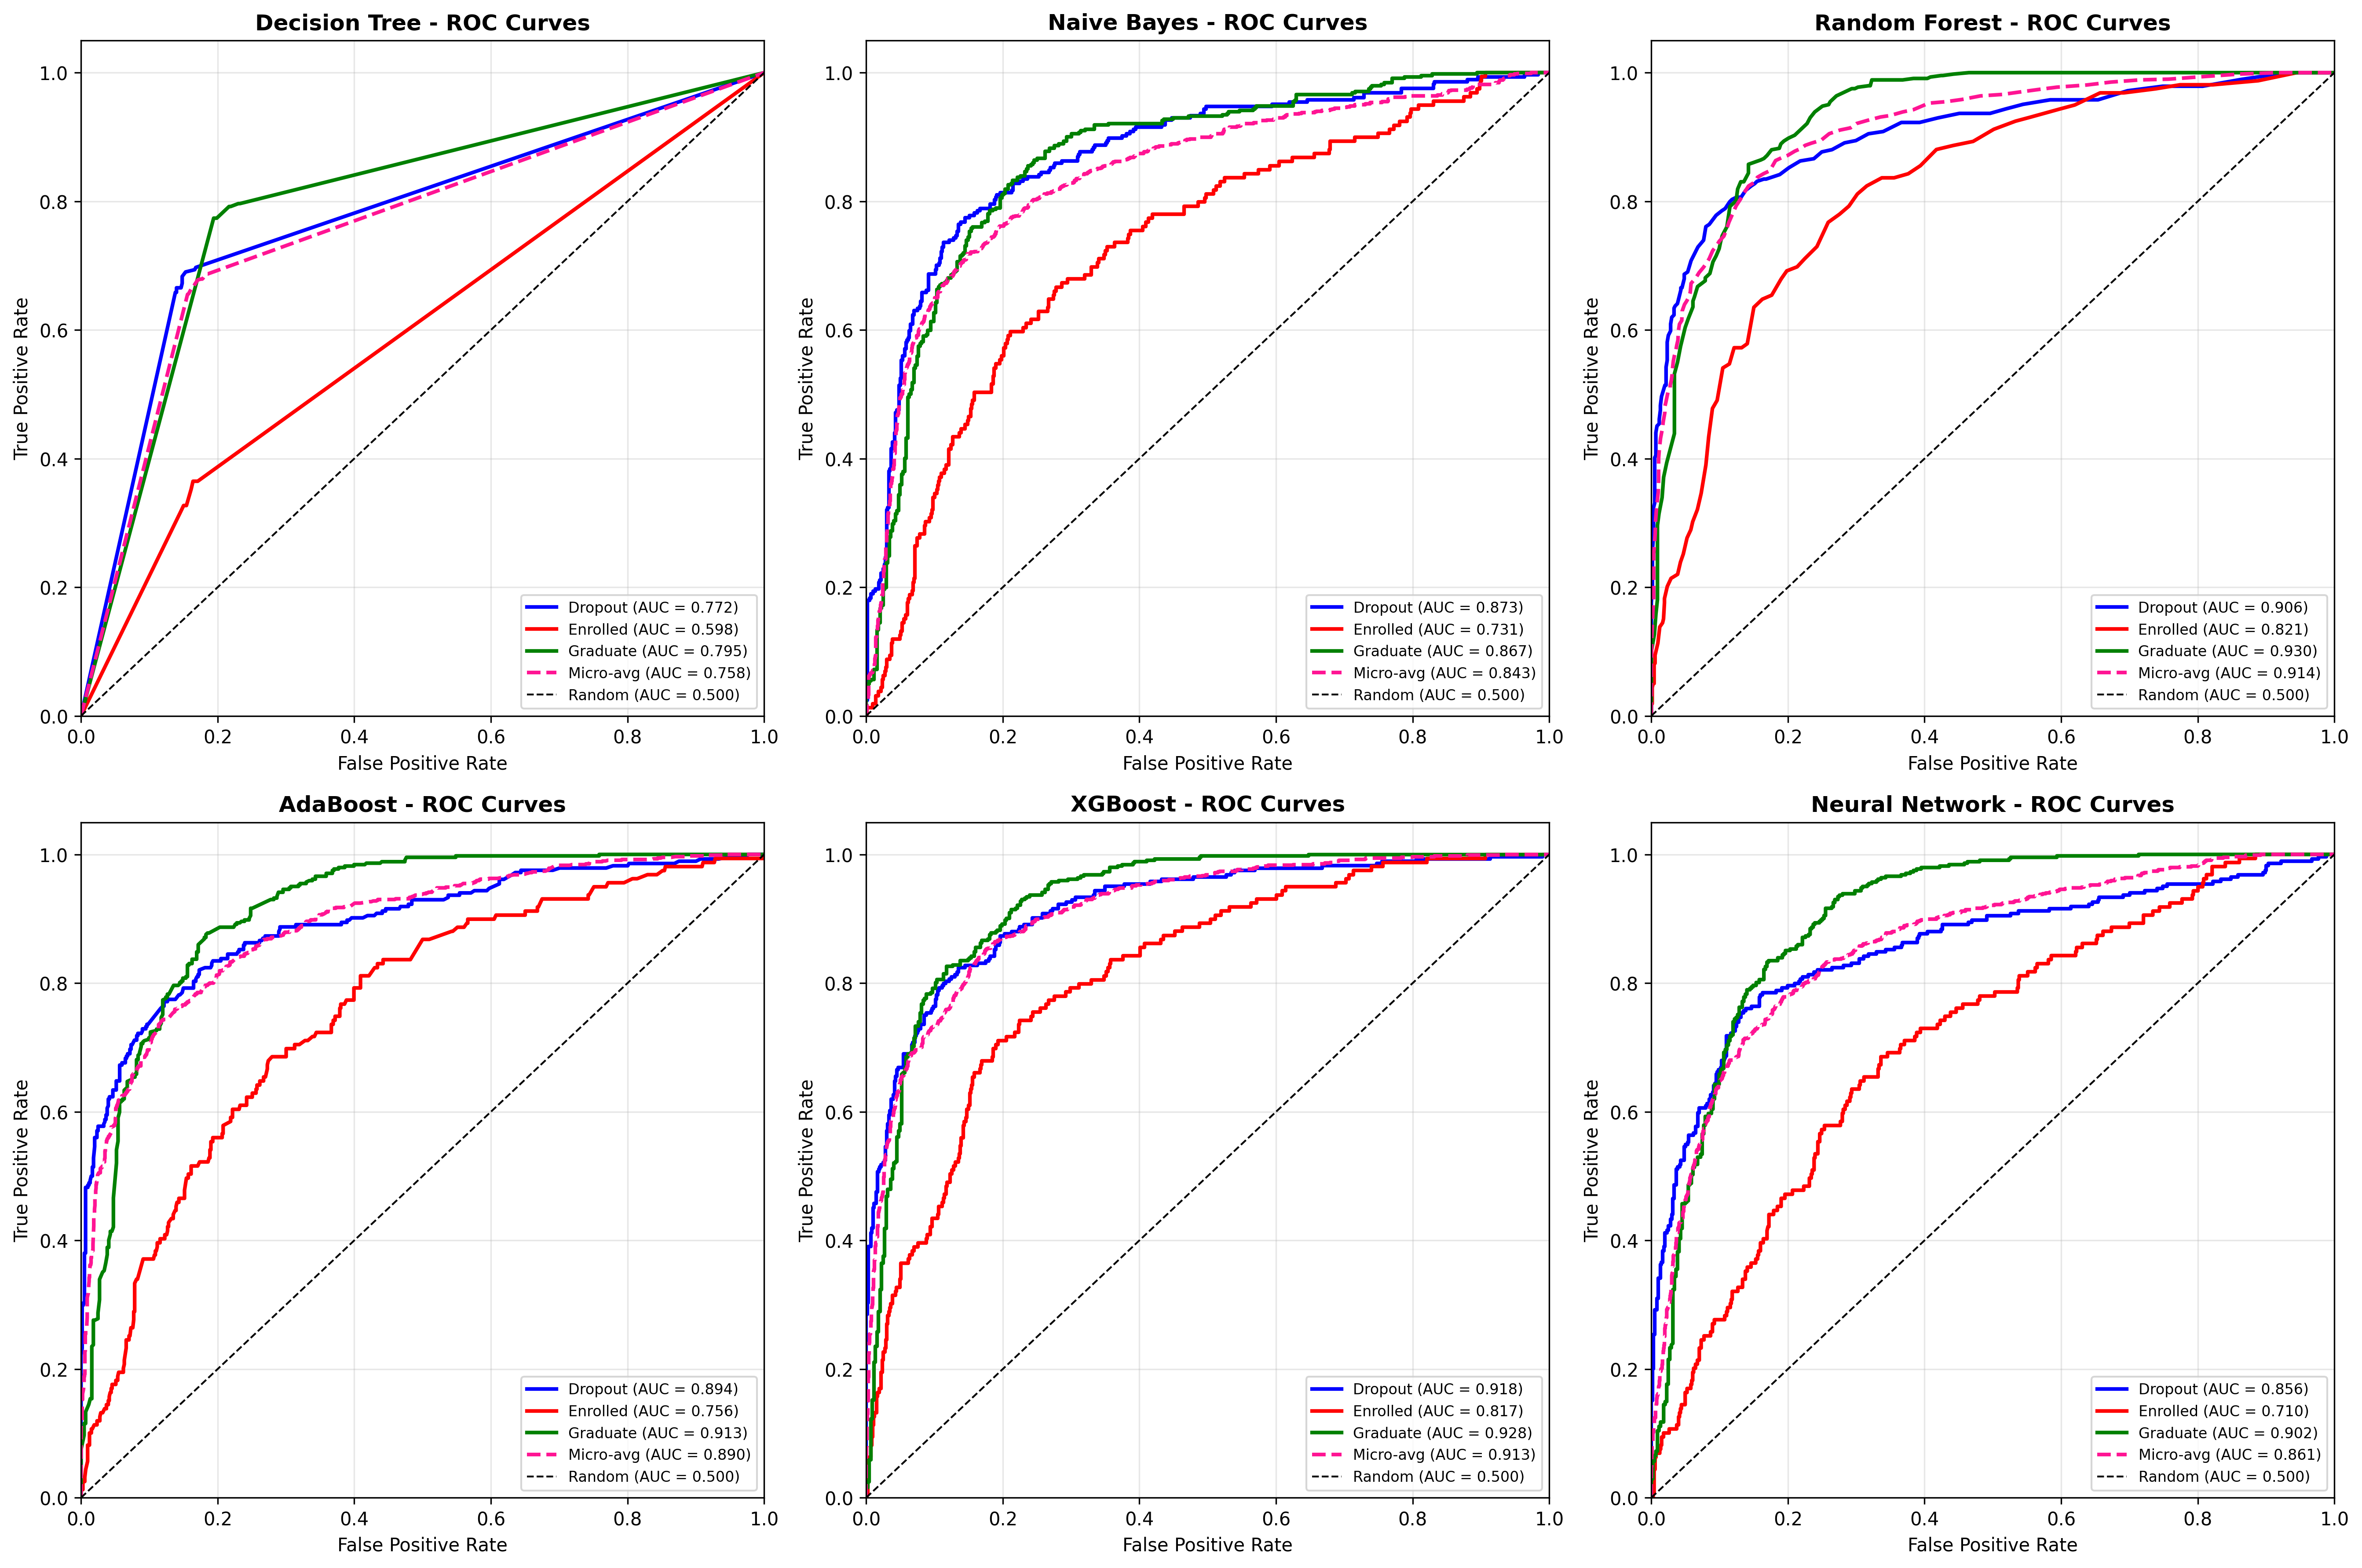
\includegraphics[width=\textwidth]{supervisor_requirements/outputs/figures/12_all_models_roc_curves.png}
    \caption{ROC curves for all models across three classes}
    \label{fig:roc_curves}
\end{figure}

\begin{table}[htbp]
\centering
\caption{Per-class AUC scores for all models}
\label{tab:auc_scores}
\begin{tabular}{lcccc}
\hline
\textbf{Model} & \textbf{Dropout} & \textbf{Enrolled} & \textbf{Graduate} & \textbf{Micro-Avg} \\
\hline
Decision Tree & 0.7719 & 0.5976 & 0.7946 & 0.7581 \\
Naive Bayes & 0.8727 & 0.7310 & 0.8670 & 0.8434 \\
Random Forest & 0.9060 & 0.8211 & 0.9301 & 0.9136 \\
AdaBoost & 0.8939 & 0.7562 & 0.9135 & 0.8896 \\
XGBoost & 0.9178 & 0.8175 & 0.9278 & 0.9133 \\
Neural Network & 0.8561 & 0.7102 & 0.9017 & 0.8608 \\
\hline
\end{tabular}
\end{table}

\subsection{10-Fold Cross-Validation}

\begin{figure}[htbp]
    \centering
    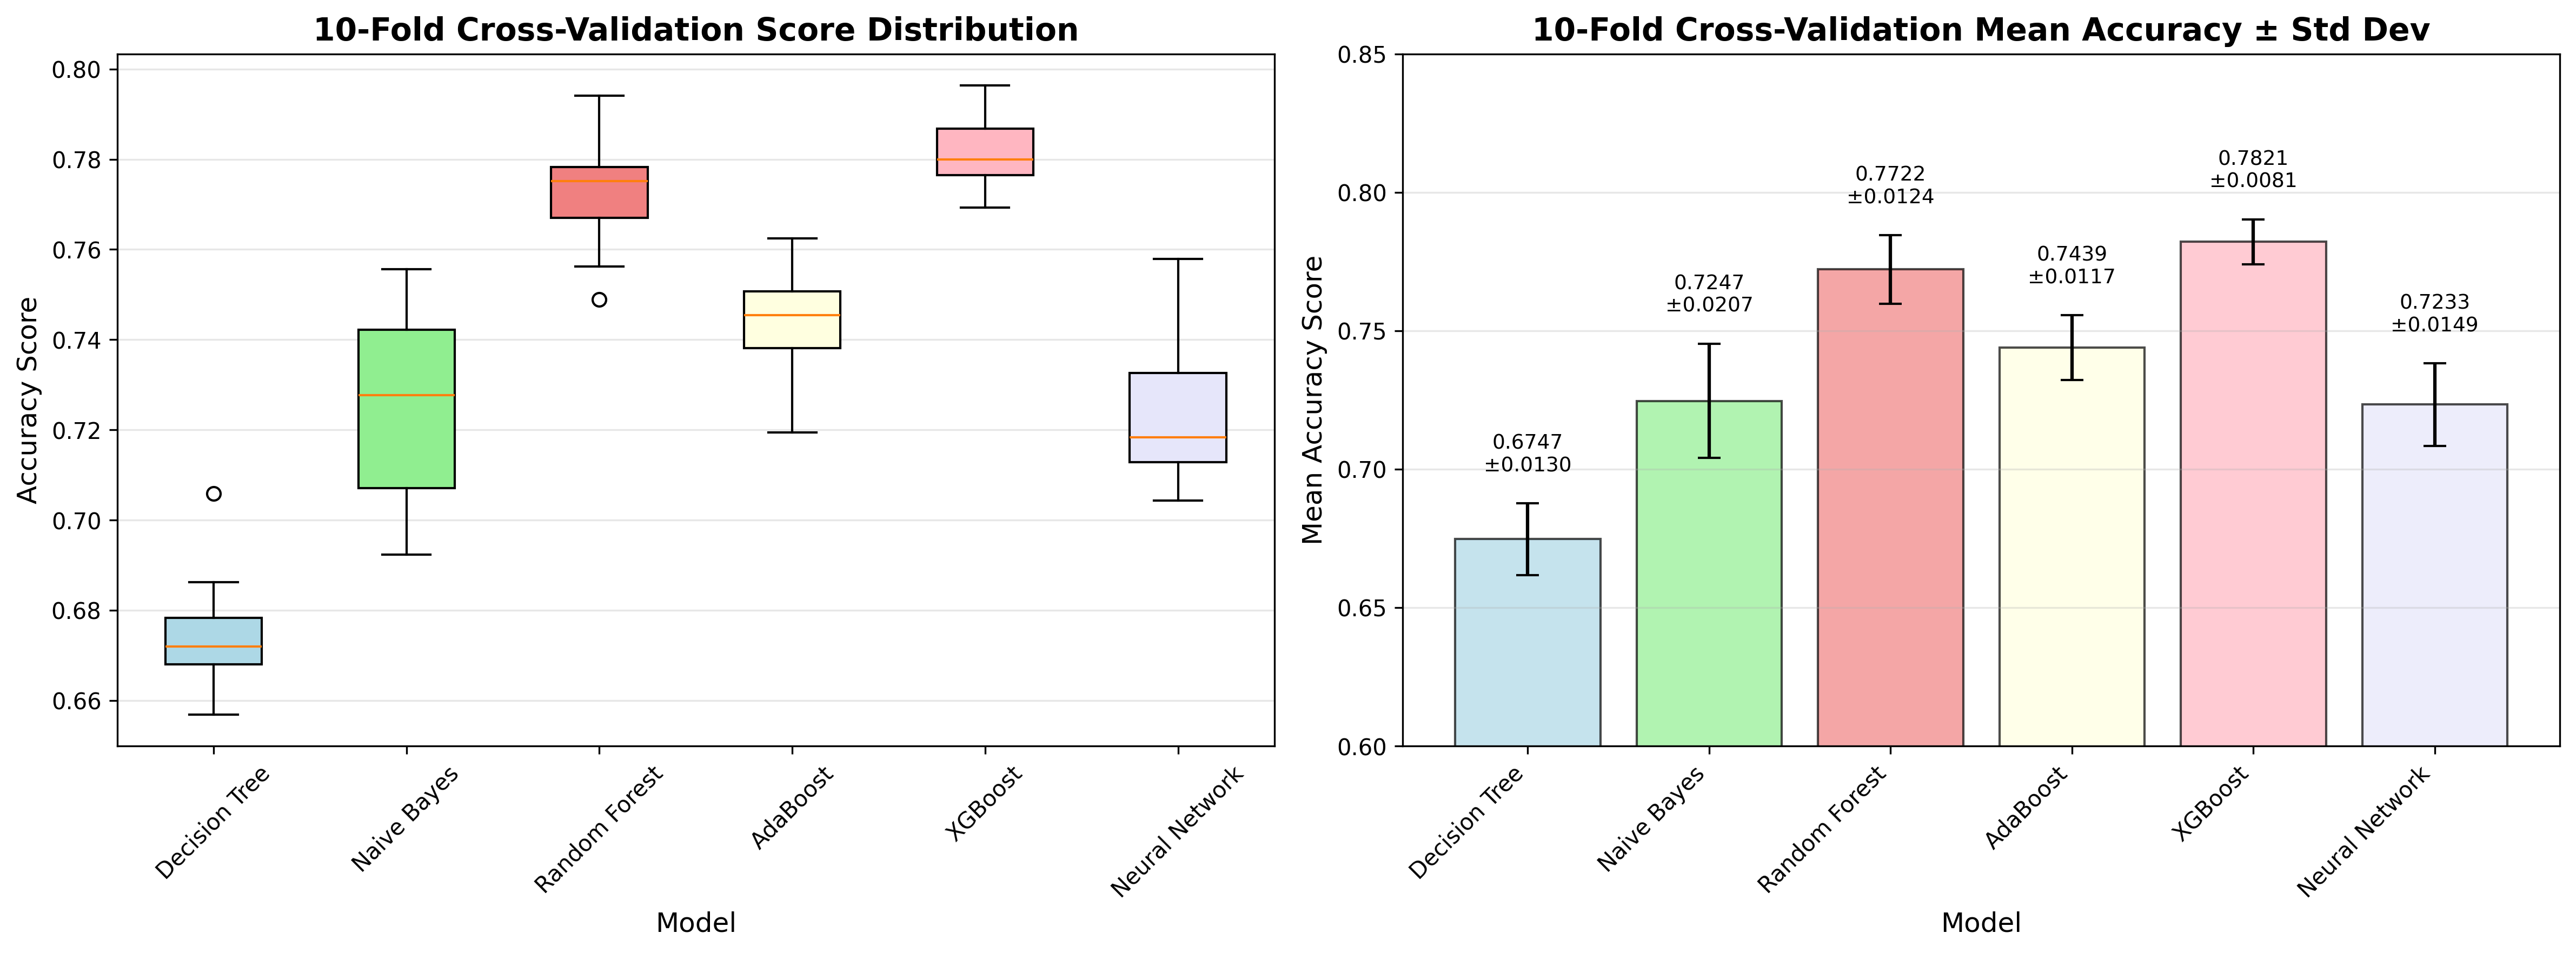
\includegraphics[width=0.85\textwidth]{supervisor_requirements/outputs/figures/12_cross_validation_results.png}
    \caption{10-fold cross-validation accuracy distribution}
    \label{fig:cross_validation}
\end{figure}

\begin{table}[htbp]
\centering
\caption{10-fold cross-validation results}
\label{tab:cv_results}
\begin{tabular}{lccc}
\hline
\textbf{Model} & \textbf{Mean Accuracy} & \textbf{Std Dev} & \textbf{95\% CI} \\
\hline
Decision Tree & 67.47\% & 1.30\% & [66.17, 68.77] \\
Naive Bayes & 72.47\% & 2.07\% & [70.40, 74.54] \\
Random Forest & 77.22\% & 1.24\% & [75.98, 78.46] \\
AdaBoost & 74.39\% & 1.17\% & [73.22, 75.56] \\
XGBoost & \textbf{78.21\%} & \textbf{0.81\%} & [77.40, 79.02] \\
Neural Network & 72.33\% & 1.49\% & [70.84, 73.82] \\
\hline
\end{tabular}
\end{table}

\section{Explainable AI Results}
\label{sec:explainable_ai}

SHAP (SHapley Additive exPlanations) analysis was performed for all six models to enhance interpretability.

\subsection{SHAP Feature Importance}

\subsubsection{Decision Tree}

\begin{figure}[htbp]
    \centering
    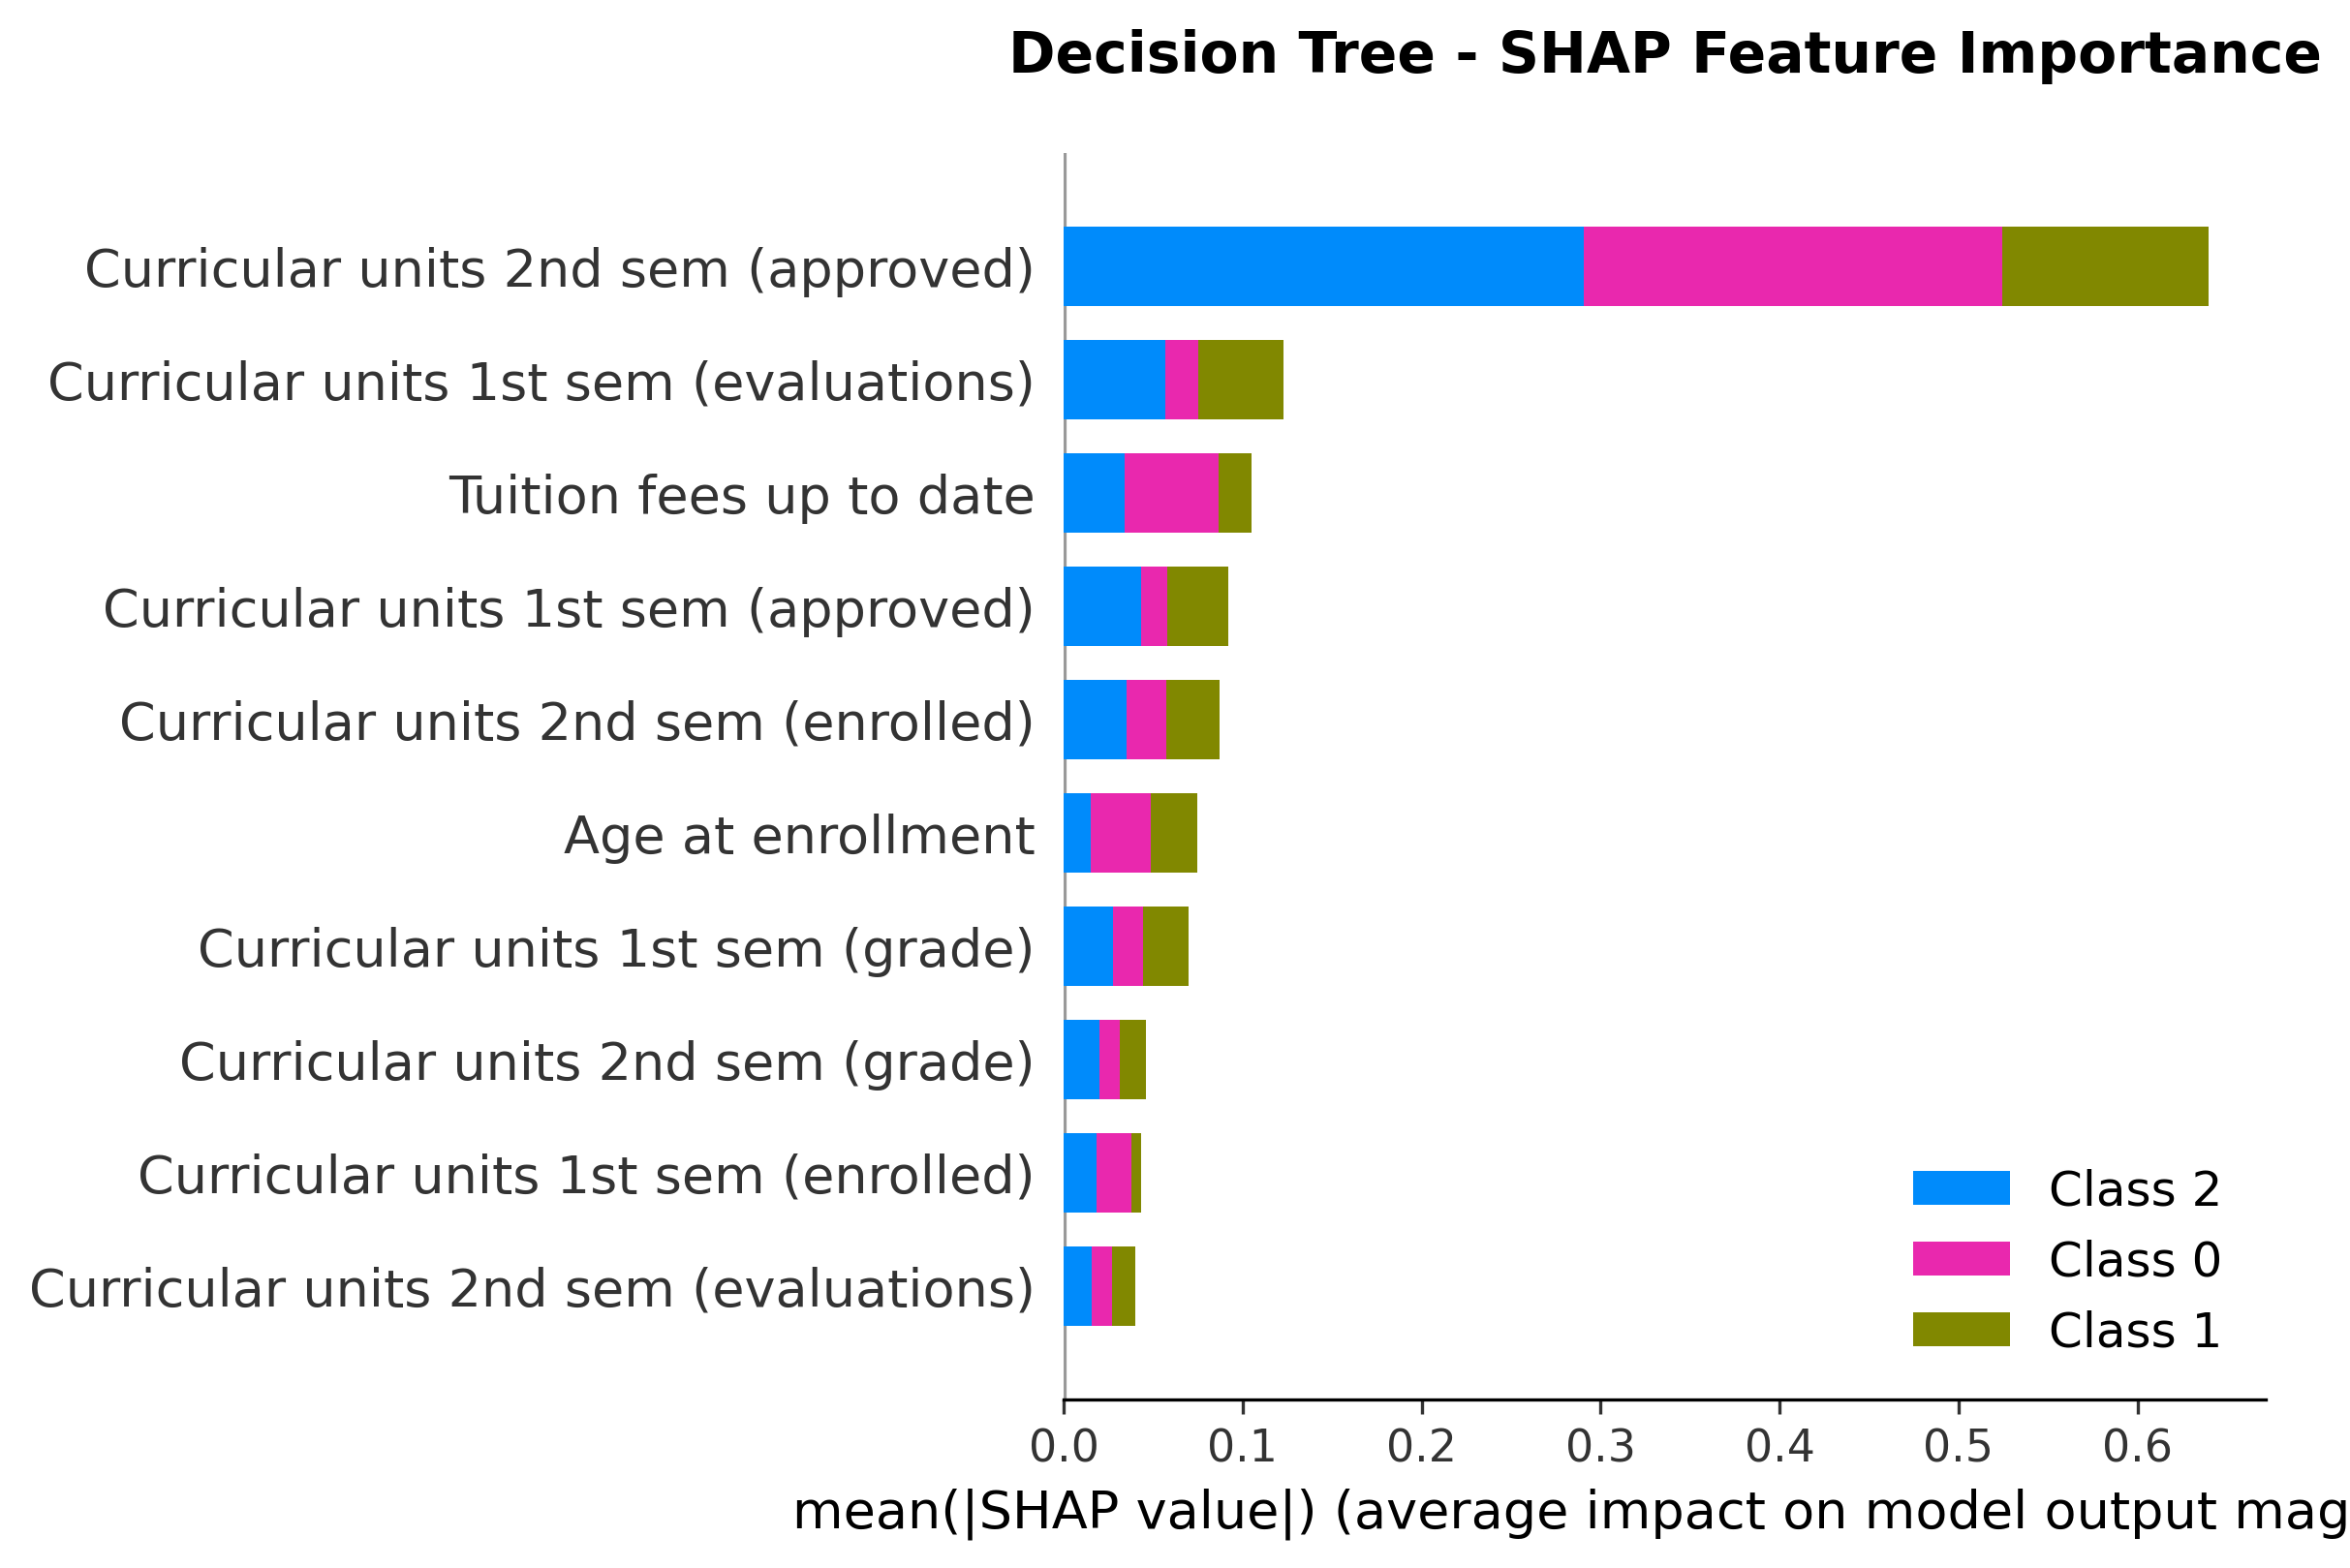
\includegraphics[width=0.85\textwidth]{supervisor_requirements/outputs/figures/11_shap_decision_tree_importance.png}
    \caption{SHAP feature importance for Decision Tree}
    \label{fig:shap_dt_importance}
\end{figure}

\begin{figure}[htbp]
    \centering
    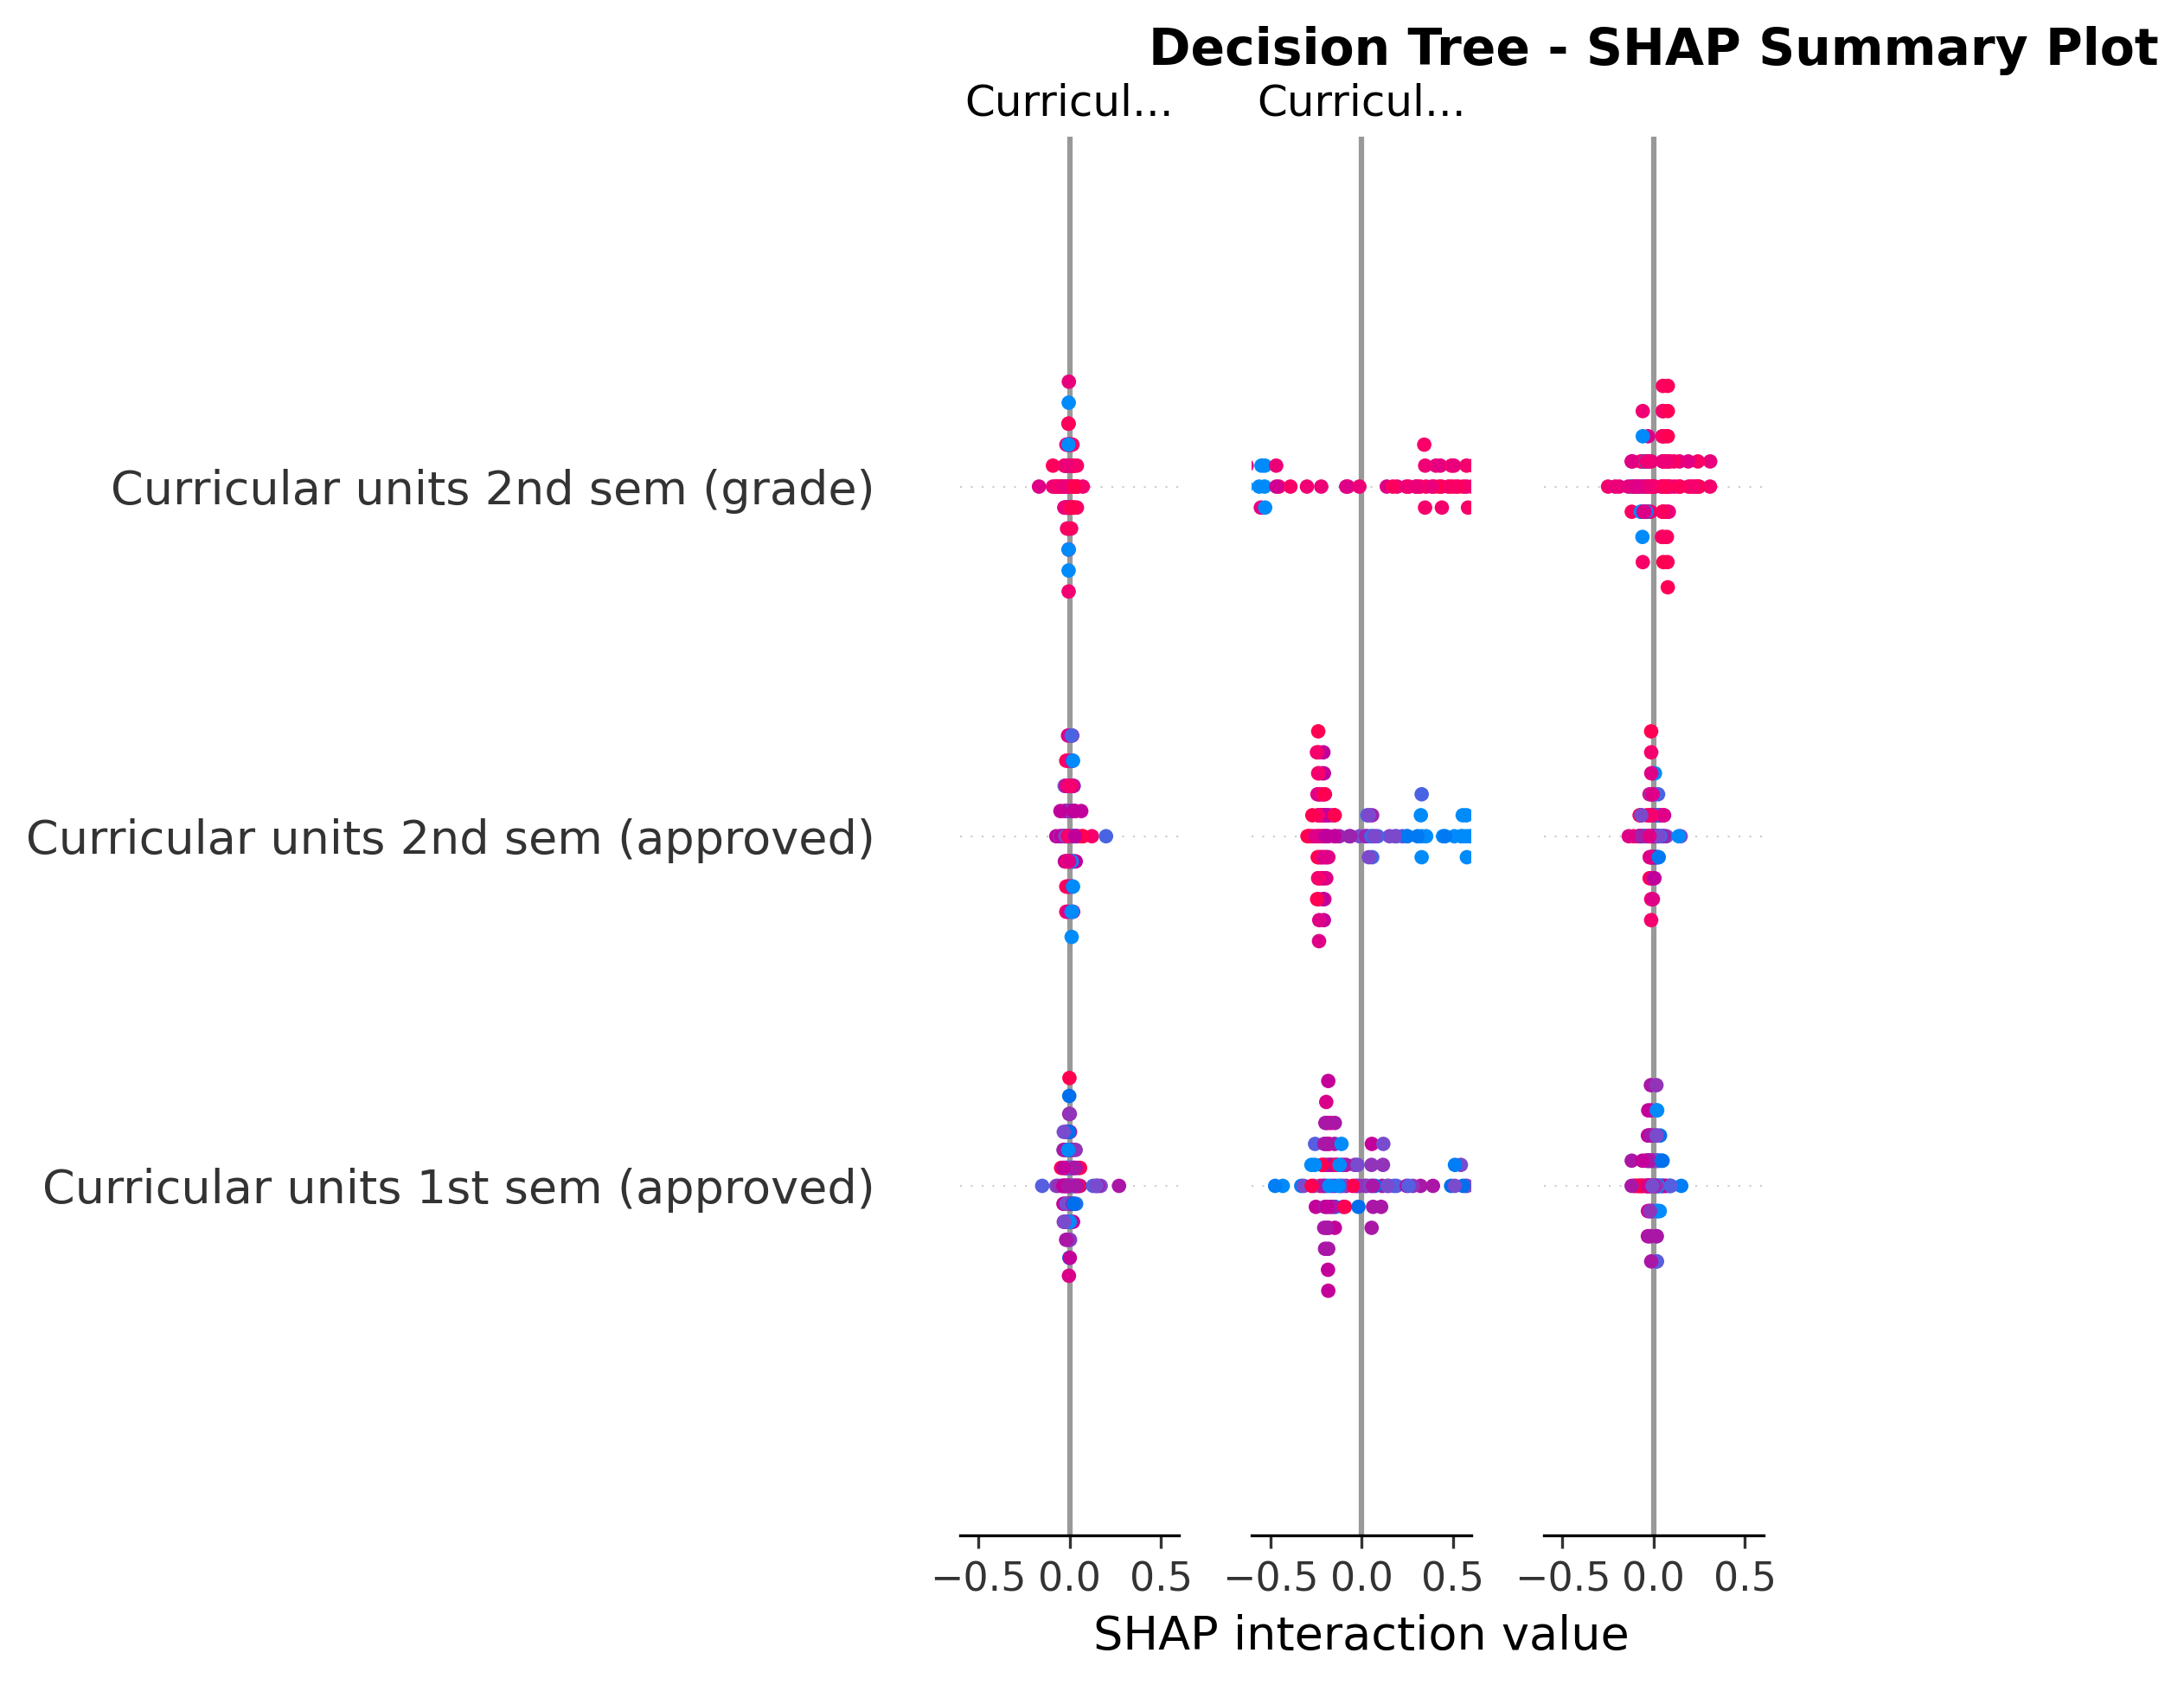
\includegraphics[width=0.85\textwidth]{supervisor_requirements/outputs/figures/11_shap_decision_tree_summary.png}
    \caption{SHAP summary plot for Decision Tree}
    \label{fig:shap_dt_summary}
\end{figure}

\subsubsection{Naive Bayes}

\begin{figure}[htbp]
    \centering
    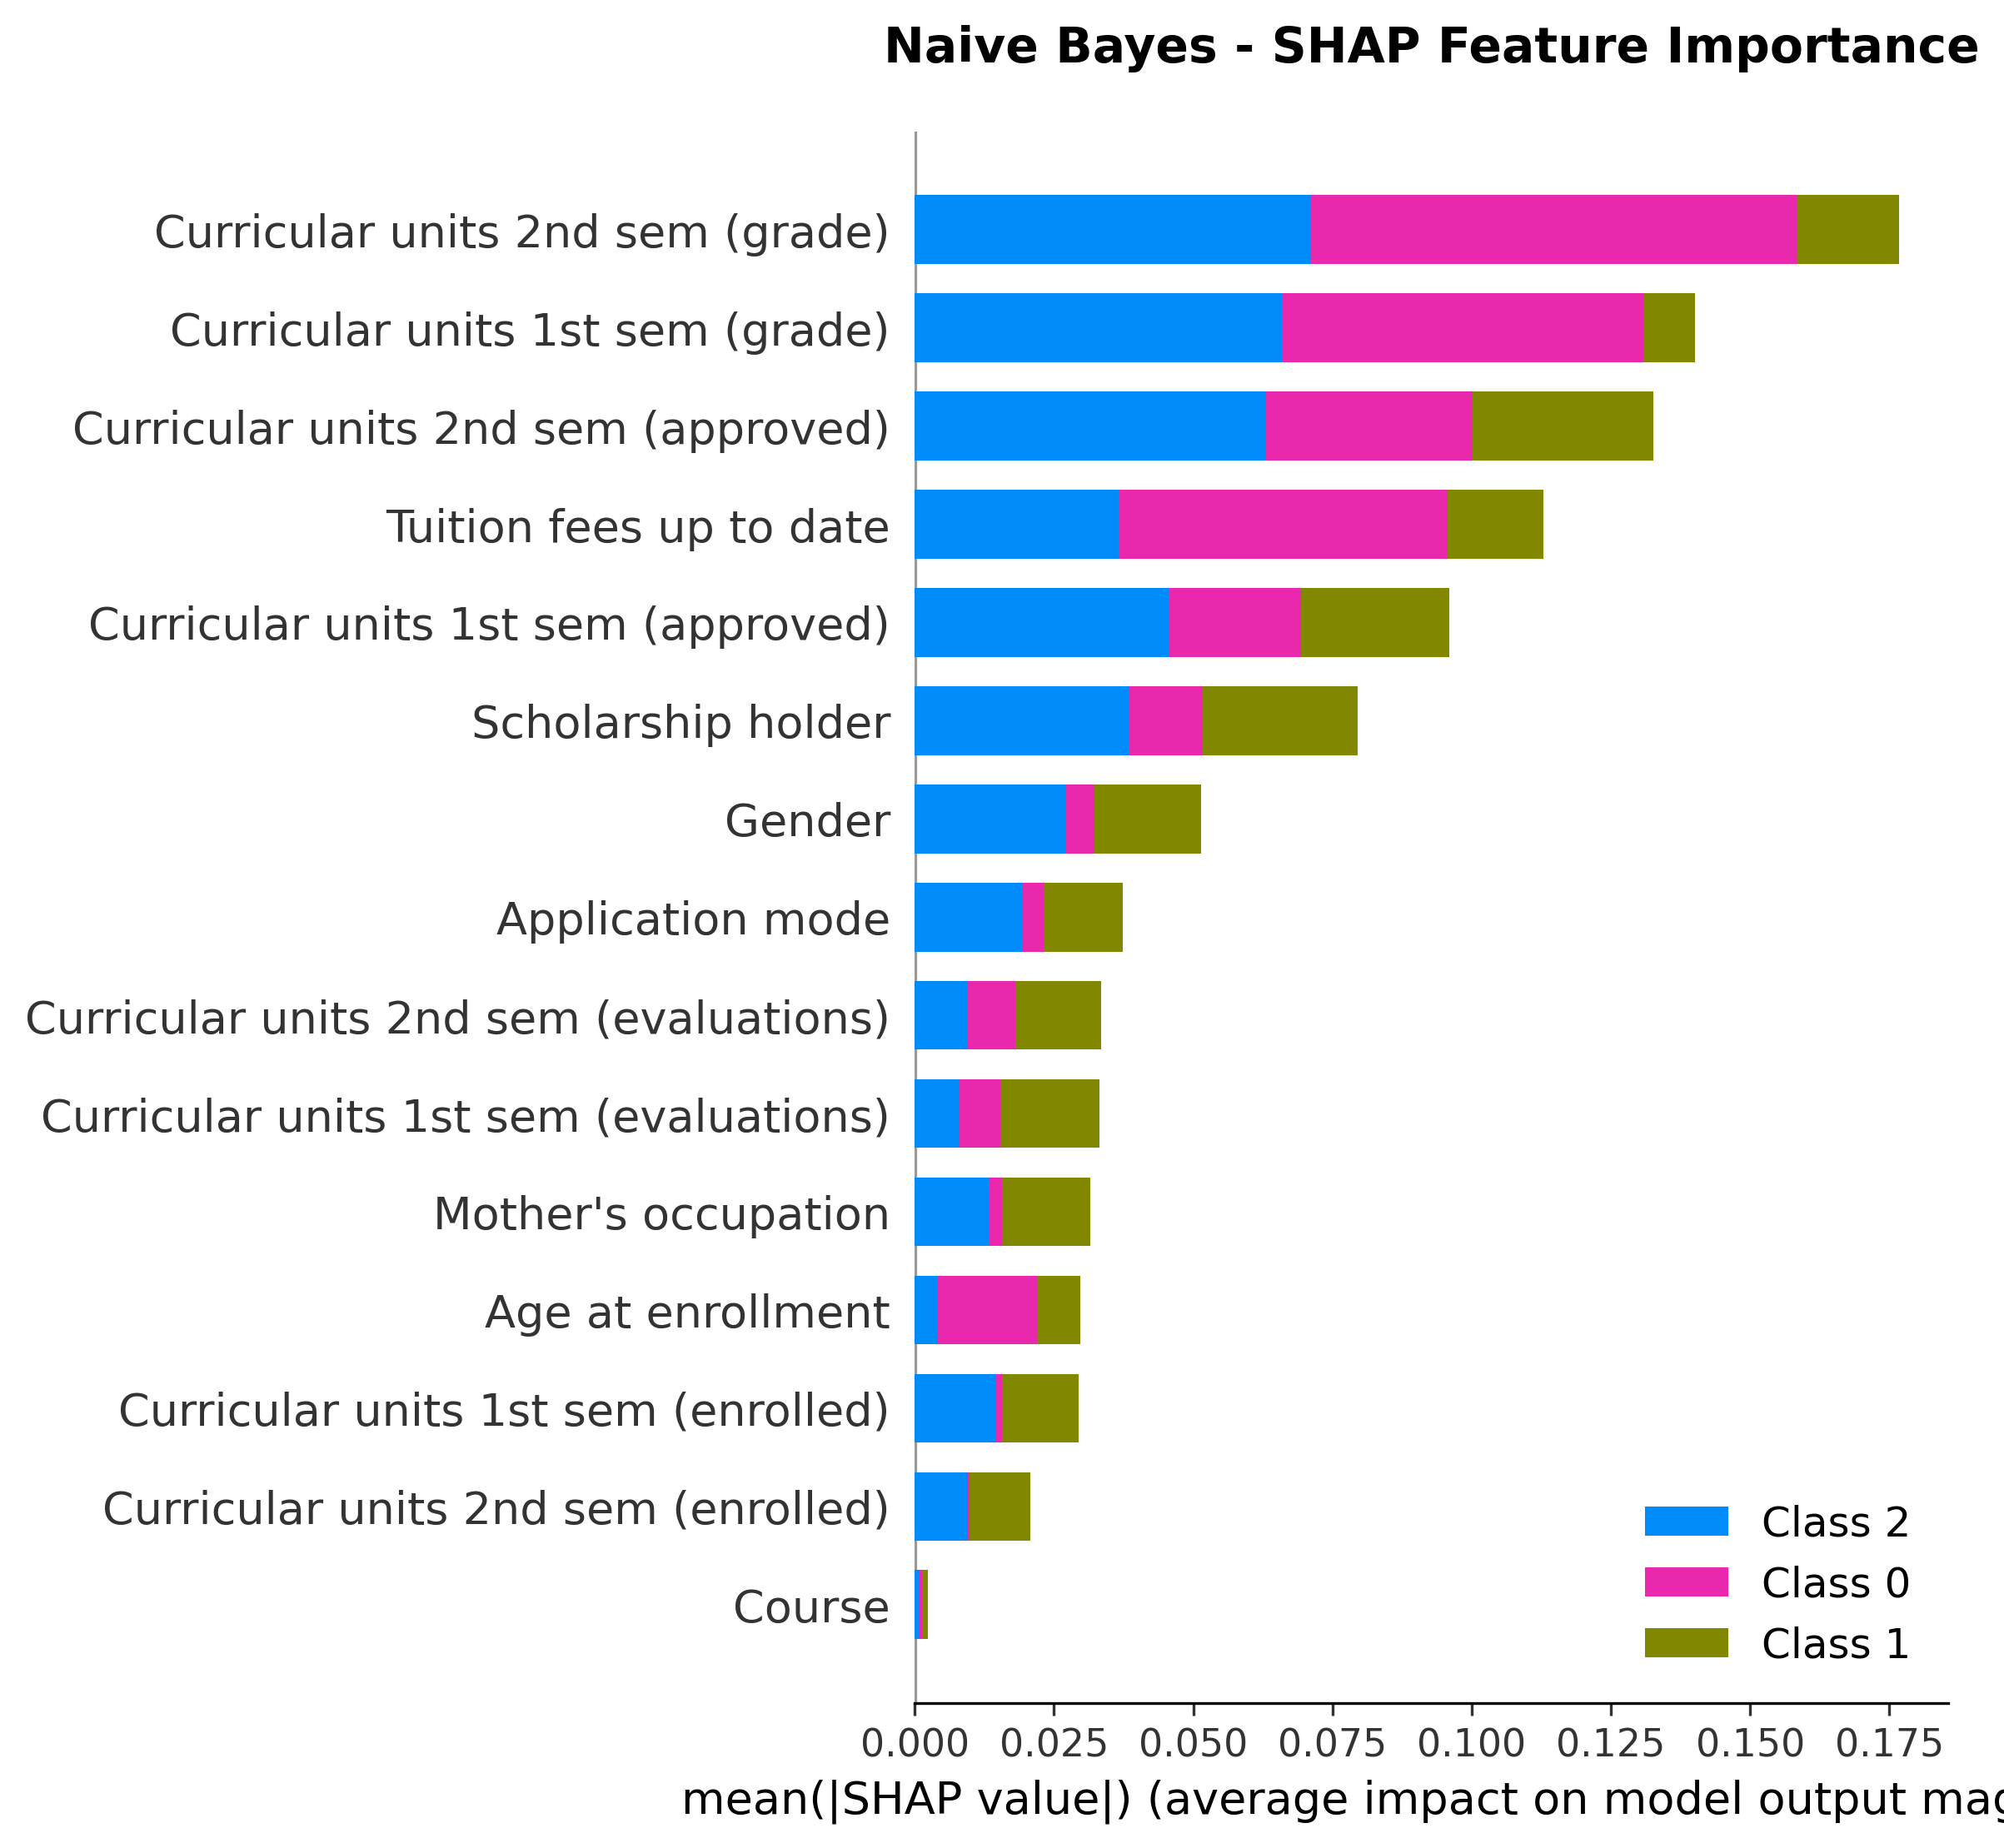
\includegraphics[width=0.85\textwidth]{supervisor_requirements/outputs/figures/11_shap_naive_bayes_importance.png}
    \caption{SHAP feature importance for Naive Bayes}
    \label{fig:shap_nb_importance}
\end{figure}

\begin{figure}[htbp]
    \centering
    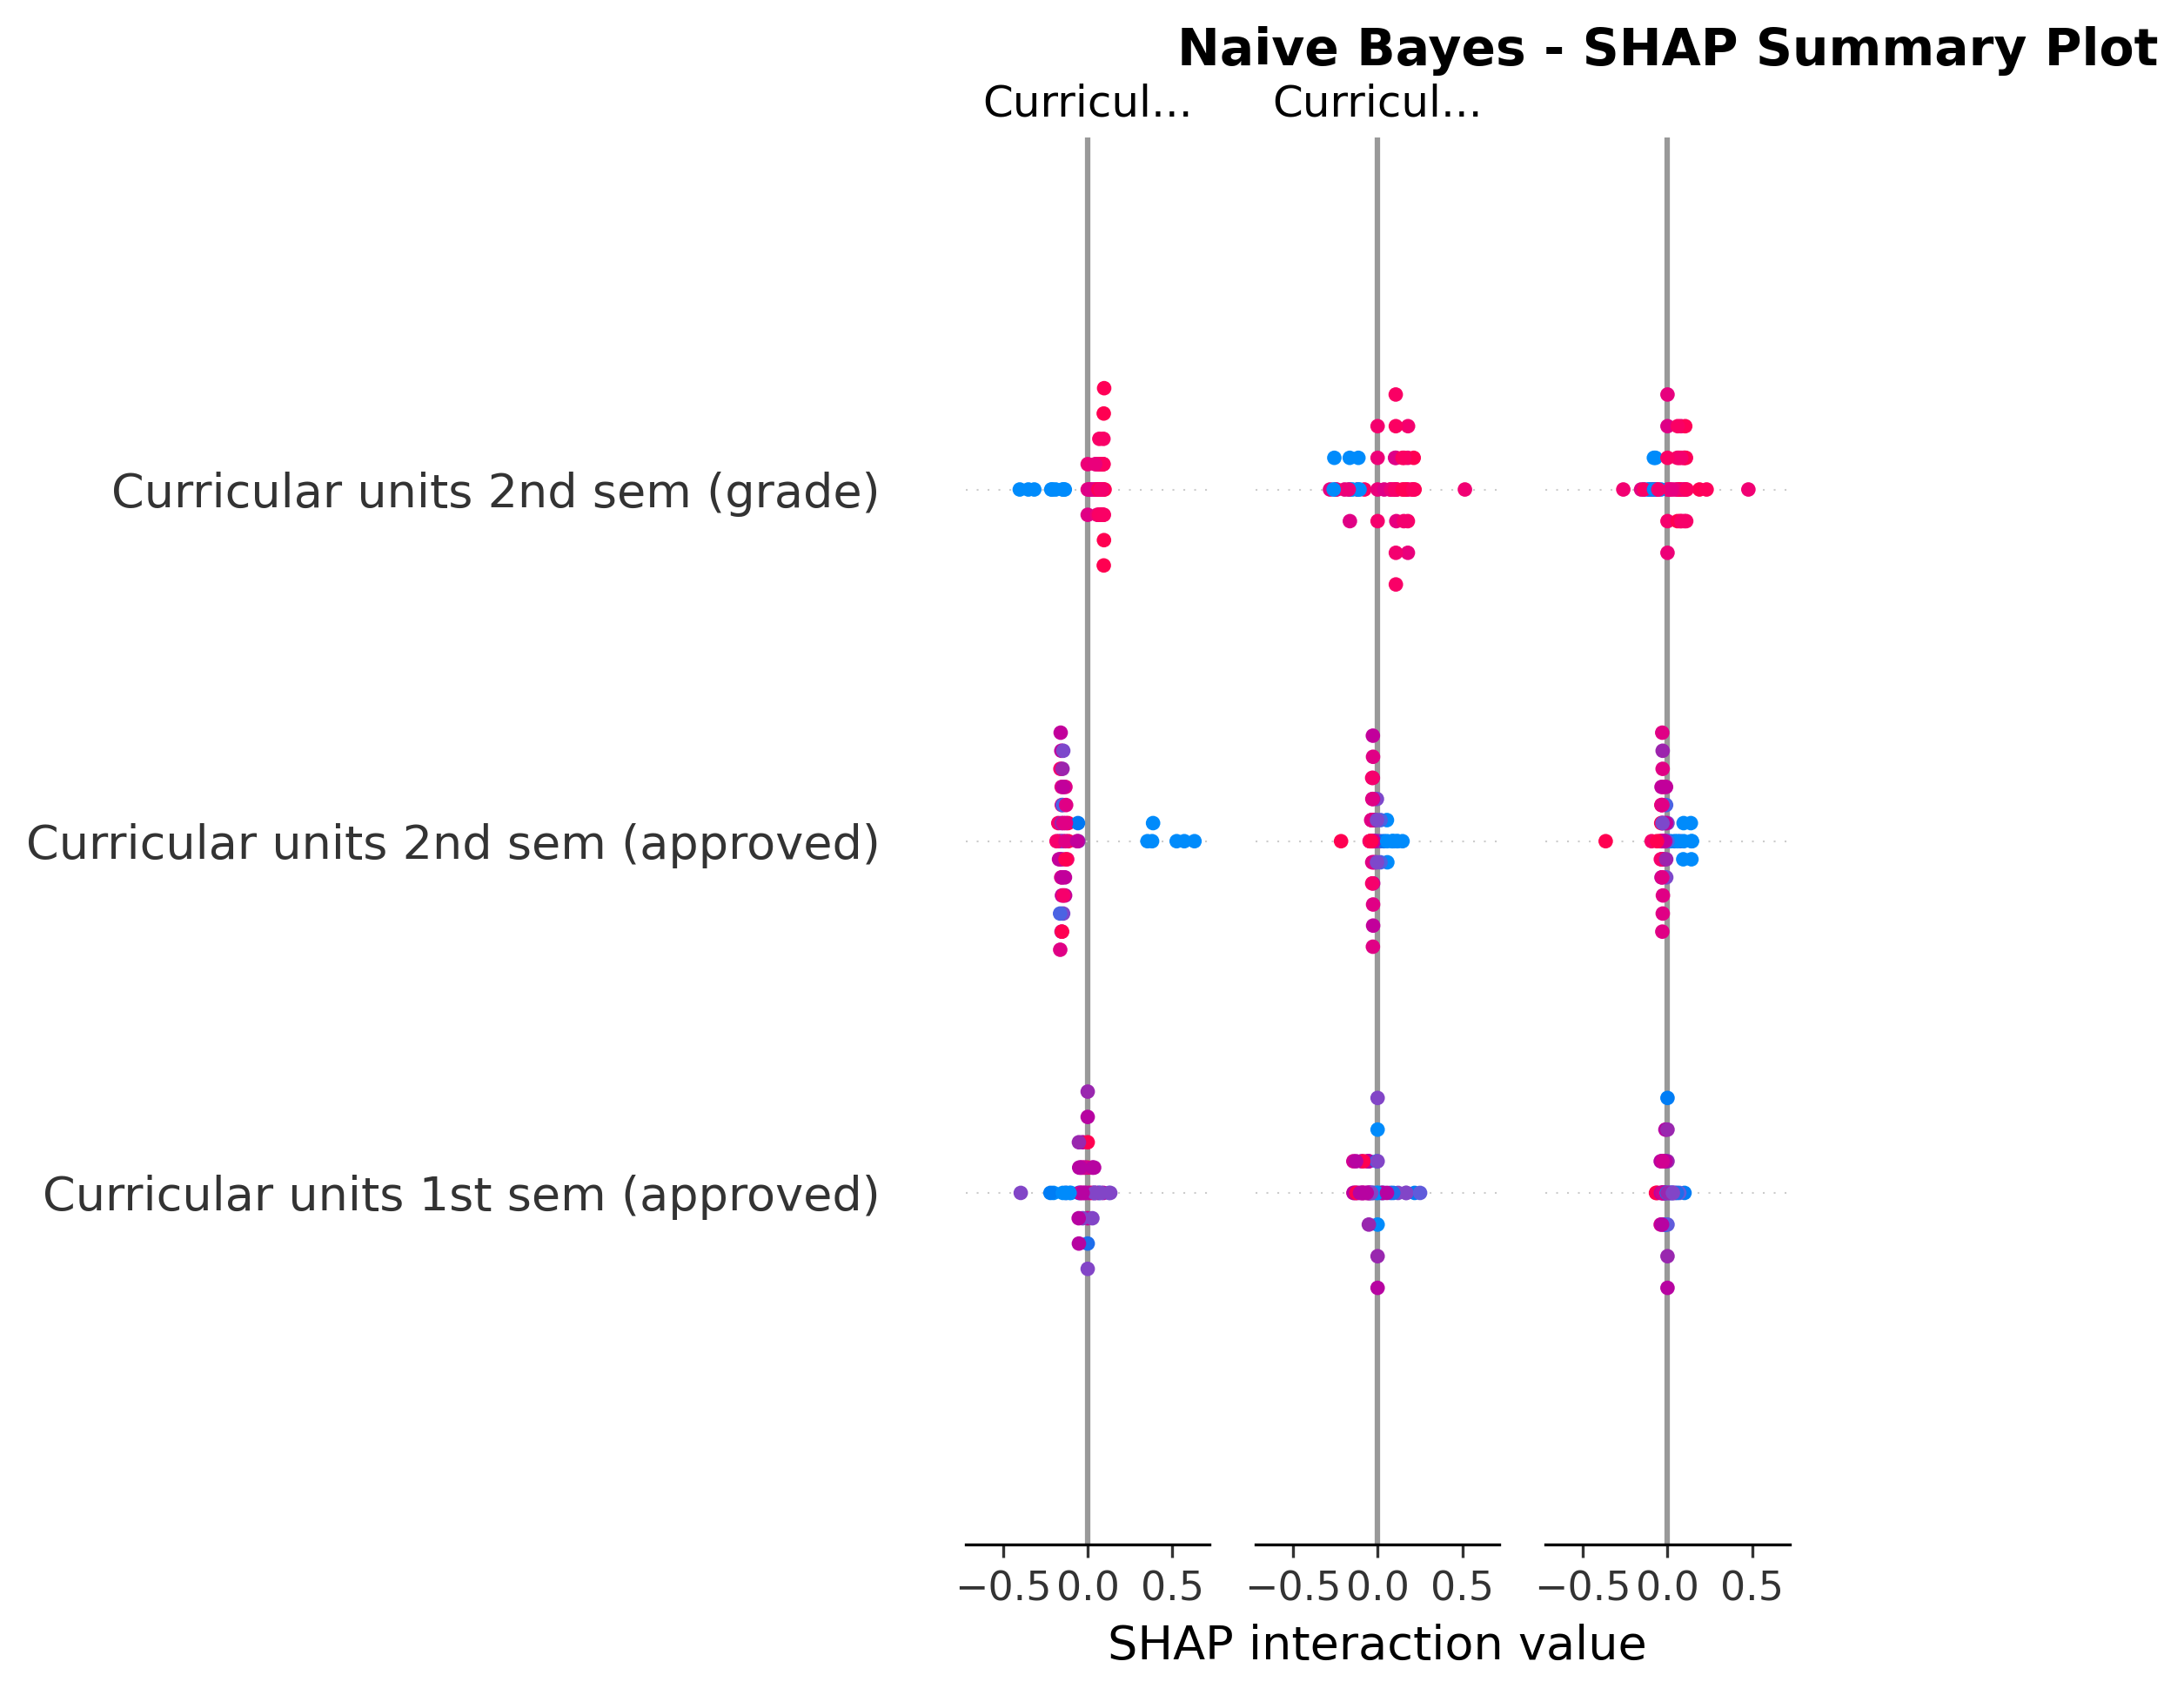
\includegraphics[width=0.85\textwidth]{supervisor_requirements/outputs/figures/11_shap_naive_bayes_summary.png}
    \caption{SHAP summary plot for Naive Bayes}
    \label{fig:shap_nb_summary}
\end{figure}

\subsubsection{Random Forest}

\begin{figure}[htbp]
    \centering
    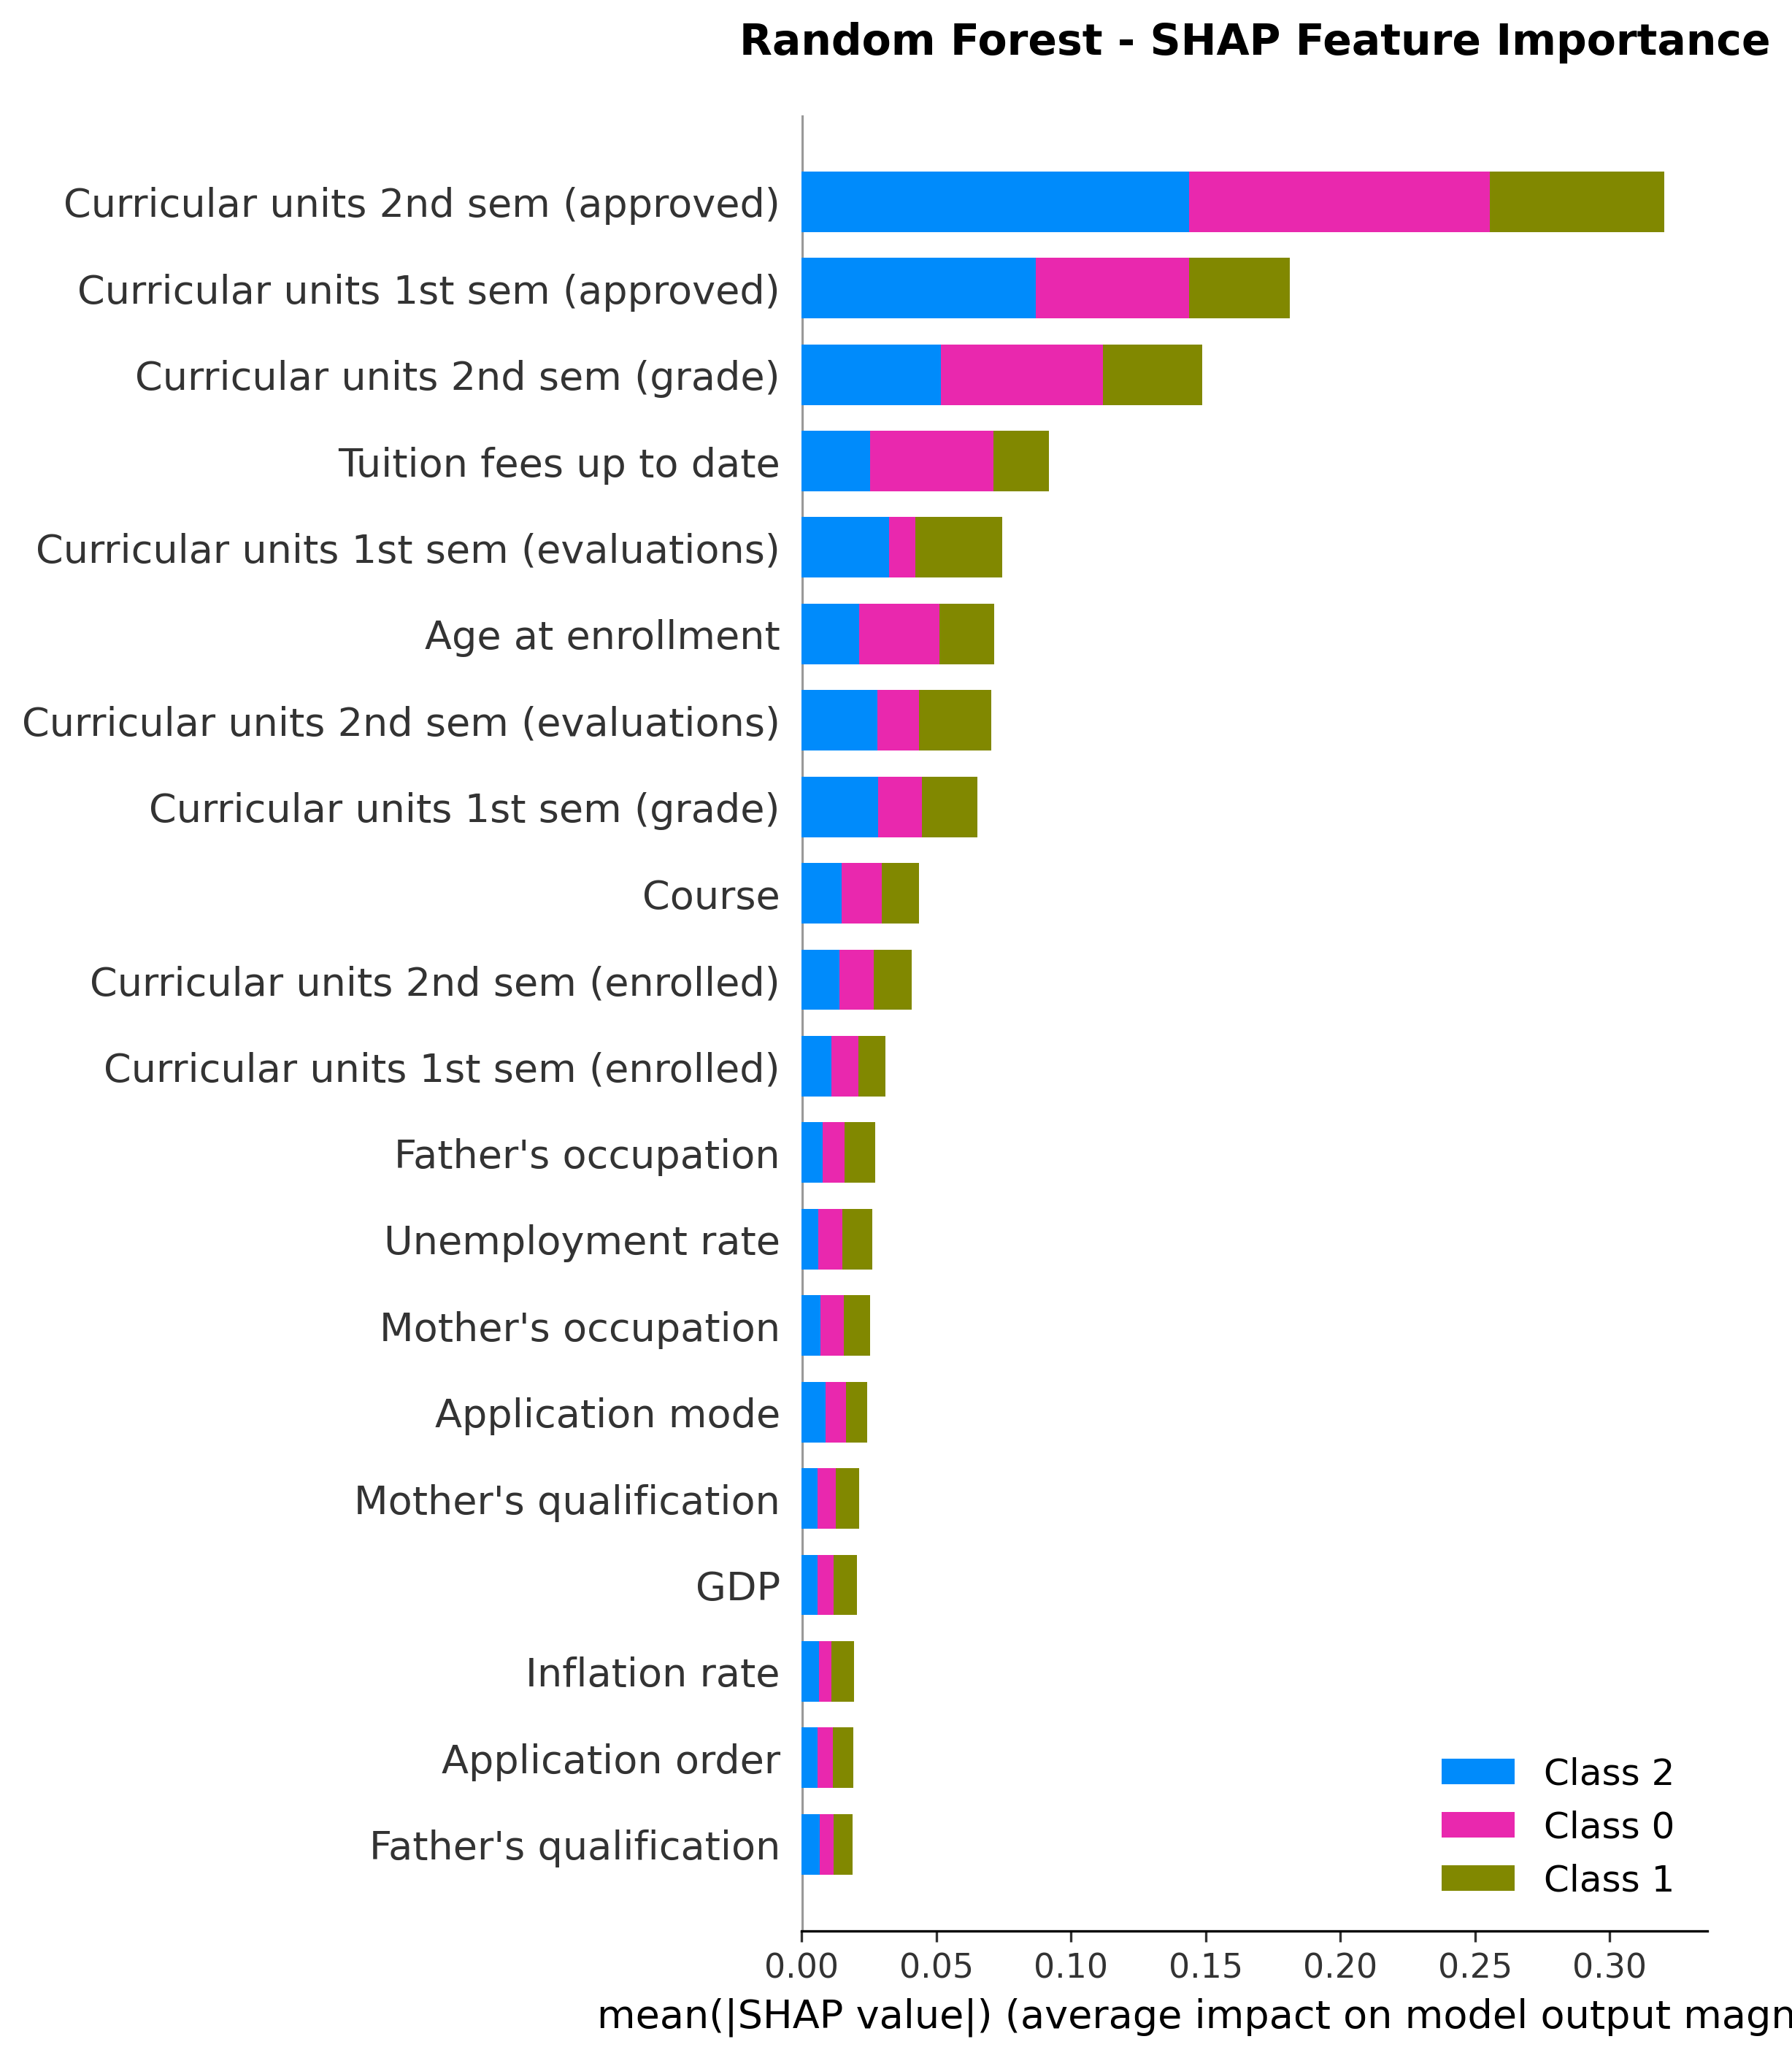
\includegraphics[width=0.85\textwidth]{supervisor_requirements/outputs/figures/11_shap_random_forest_importance.png}
    \caption{SHAP feature importance for Random Forest}
    \label{fig:shap_rf_importance}
\end{figure}

\begin{figure}[htbp]
    \centering
    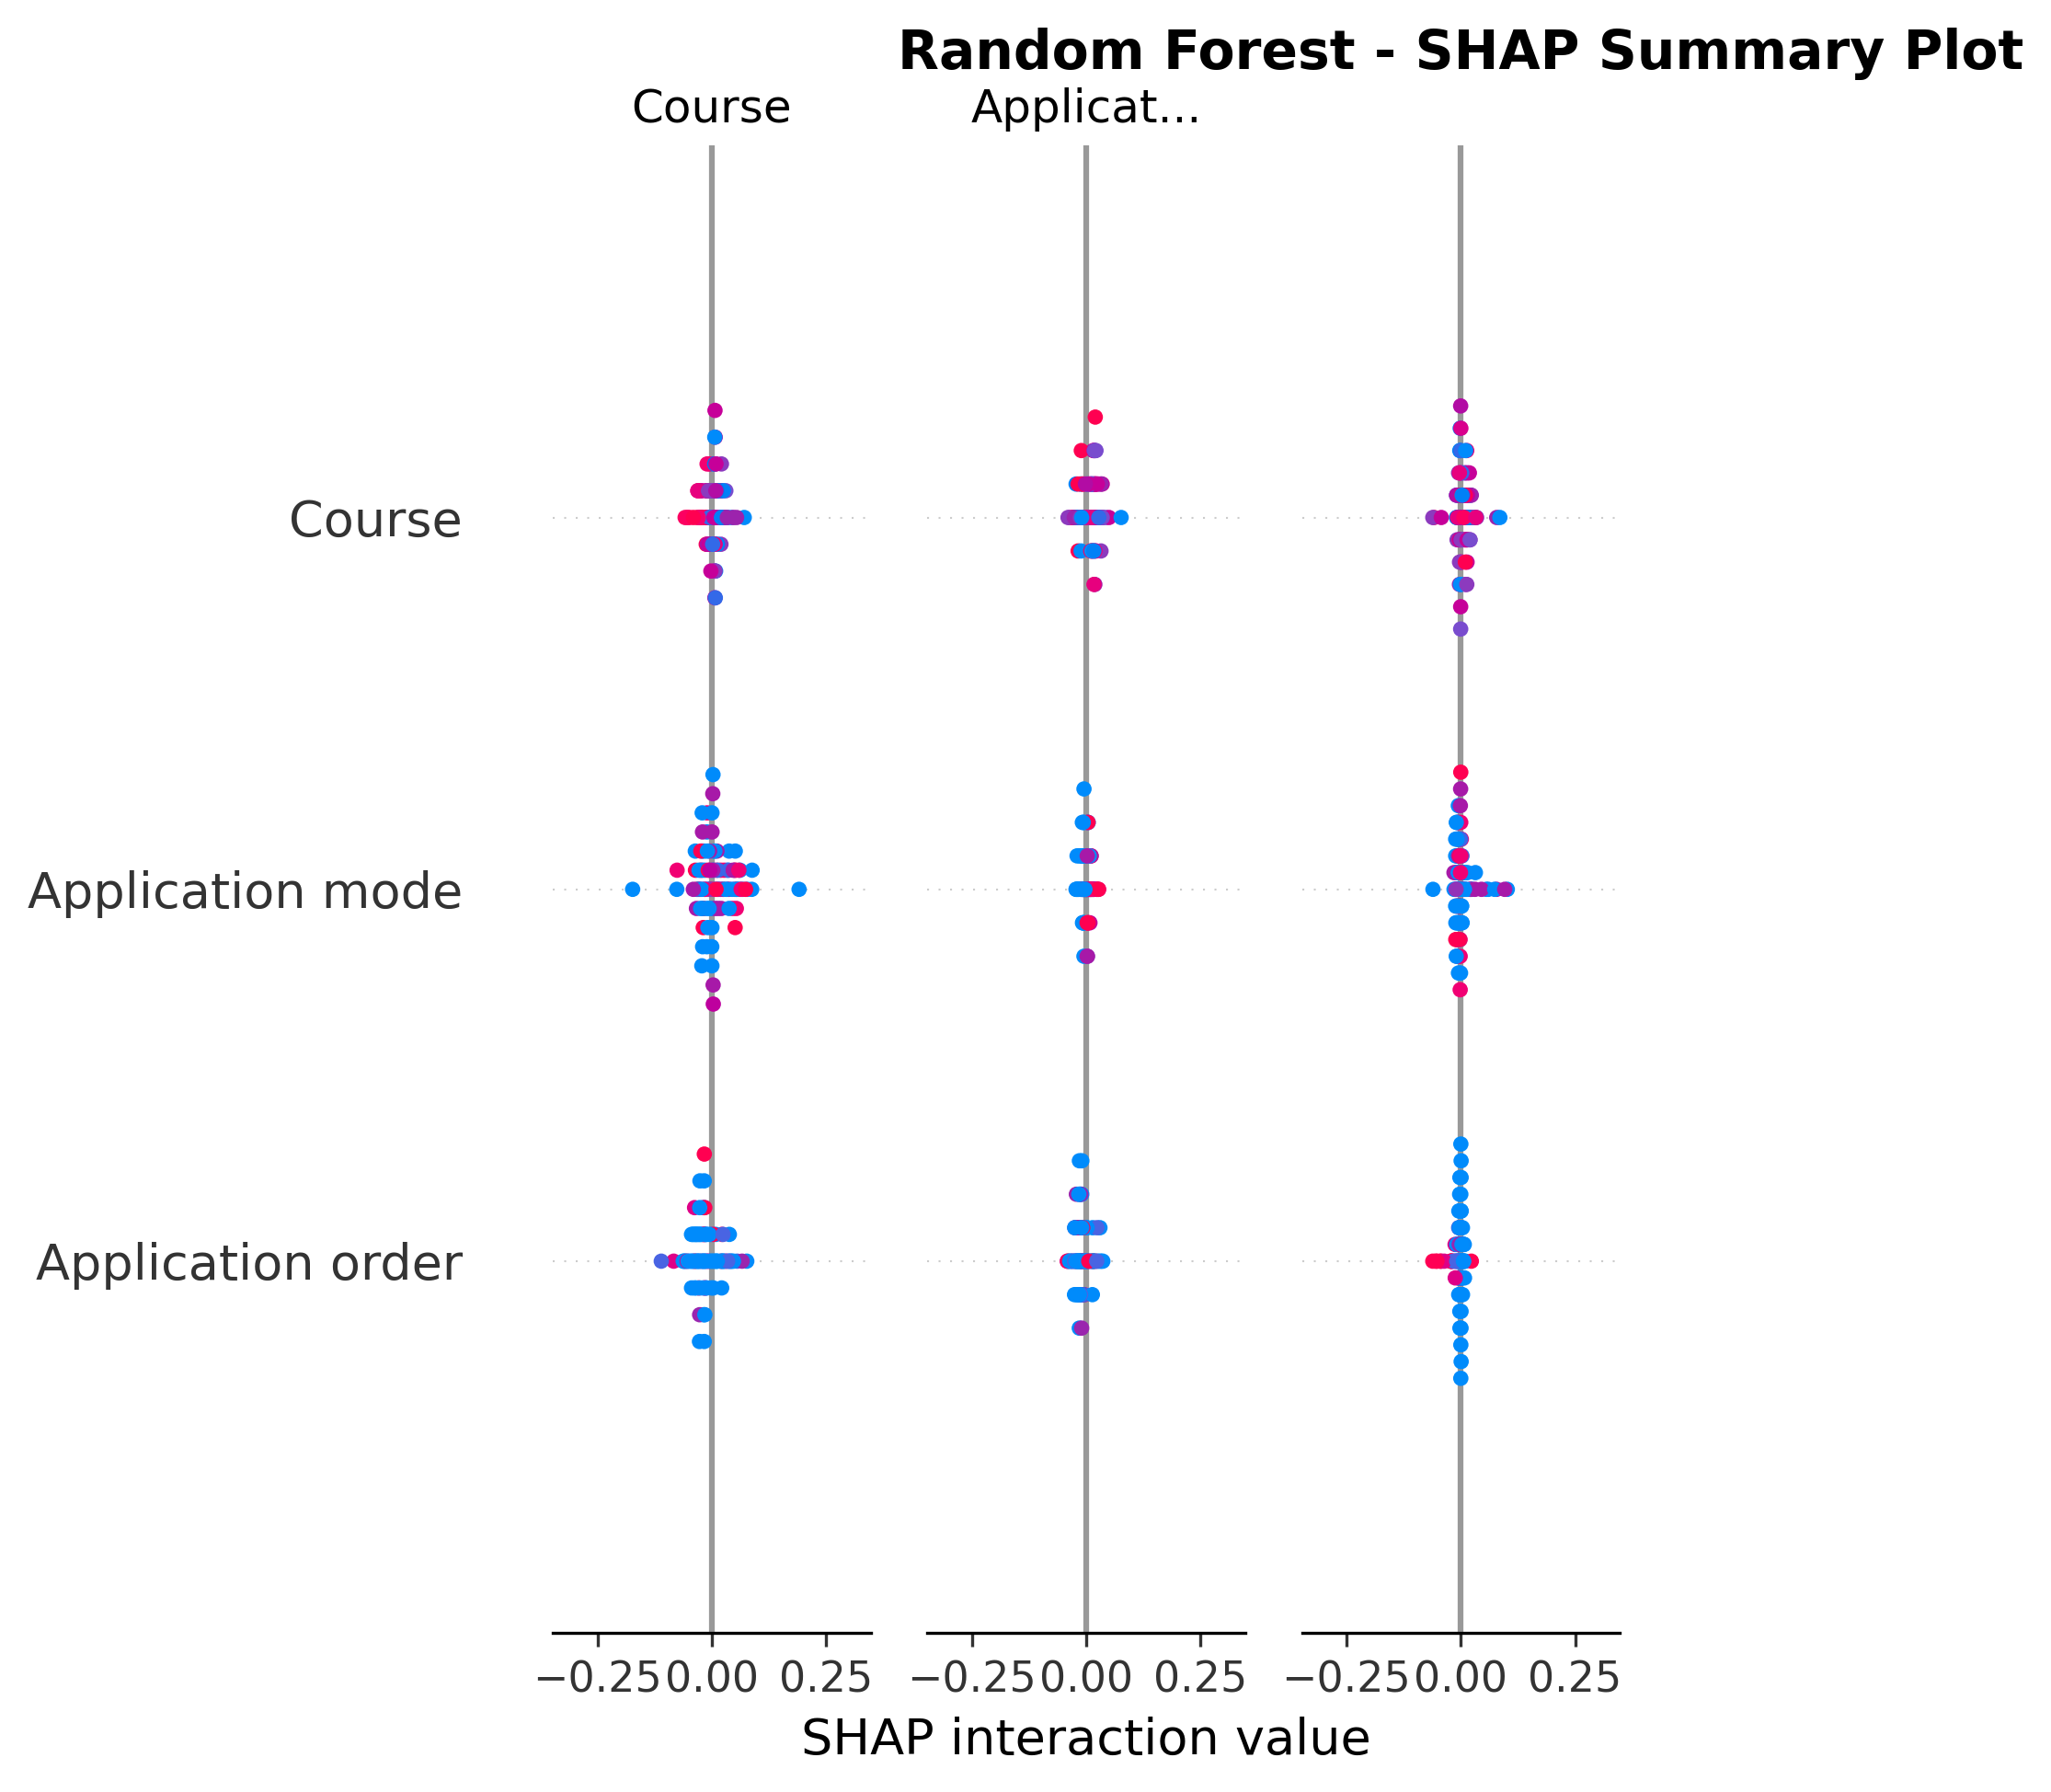
\includegraphics[width=0.85\textwidth]{supervisor_requirements/outputs/figures/11_shap_random_forest_summary.png}
    \caption{SHAP summary plot for Random Forest}
    \label{fig:shap_rf_summary}
\end{figure}

\subsubsection{AdaBoost}

\begin{figure}[htbp]
    \centering
    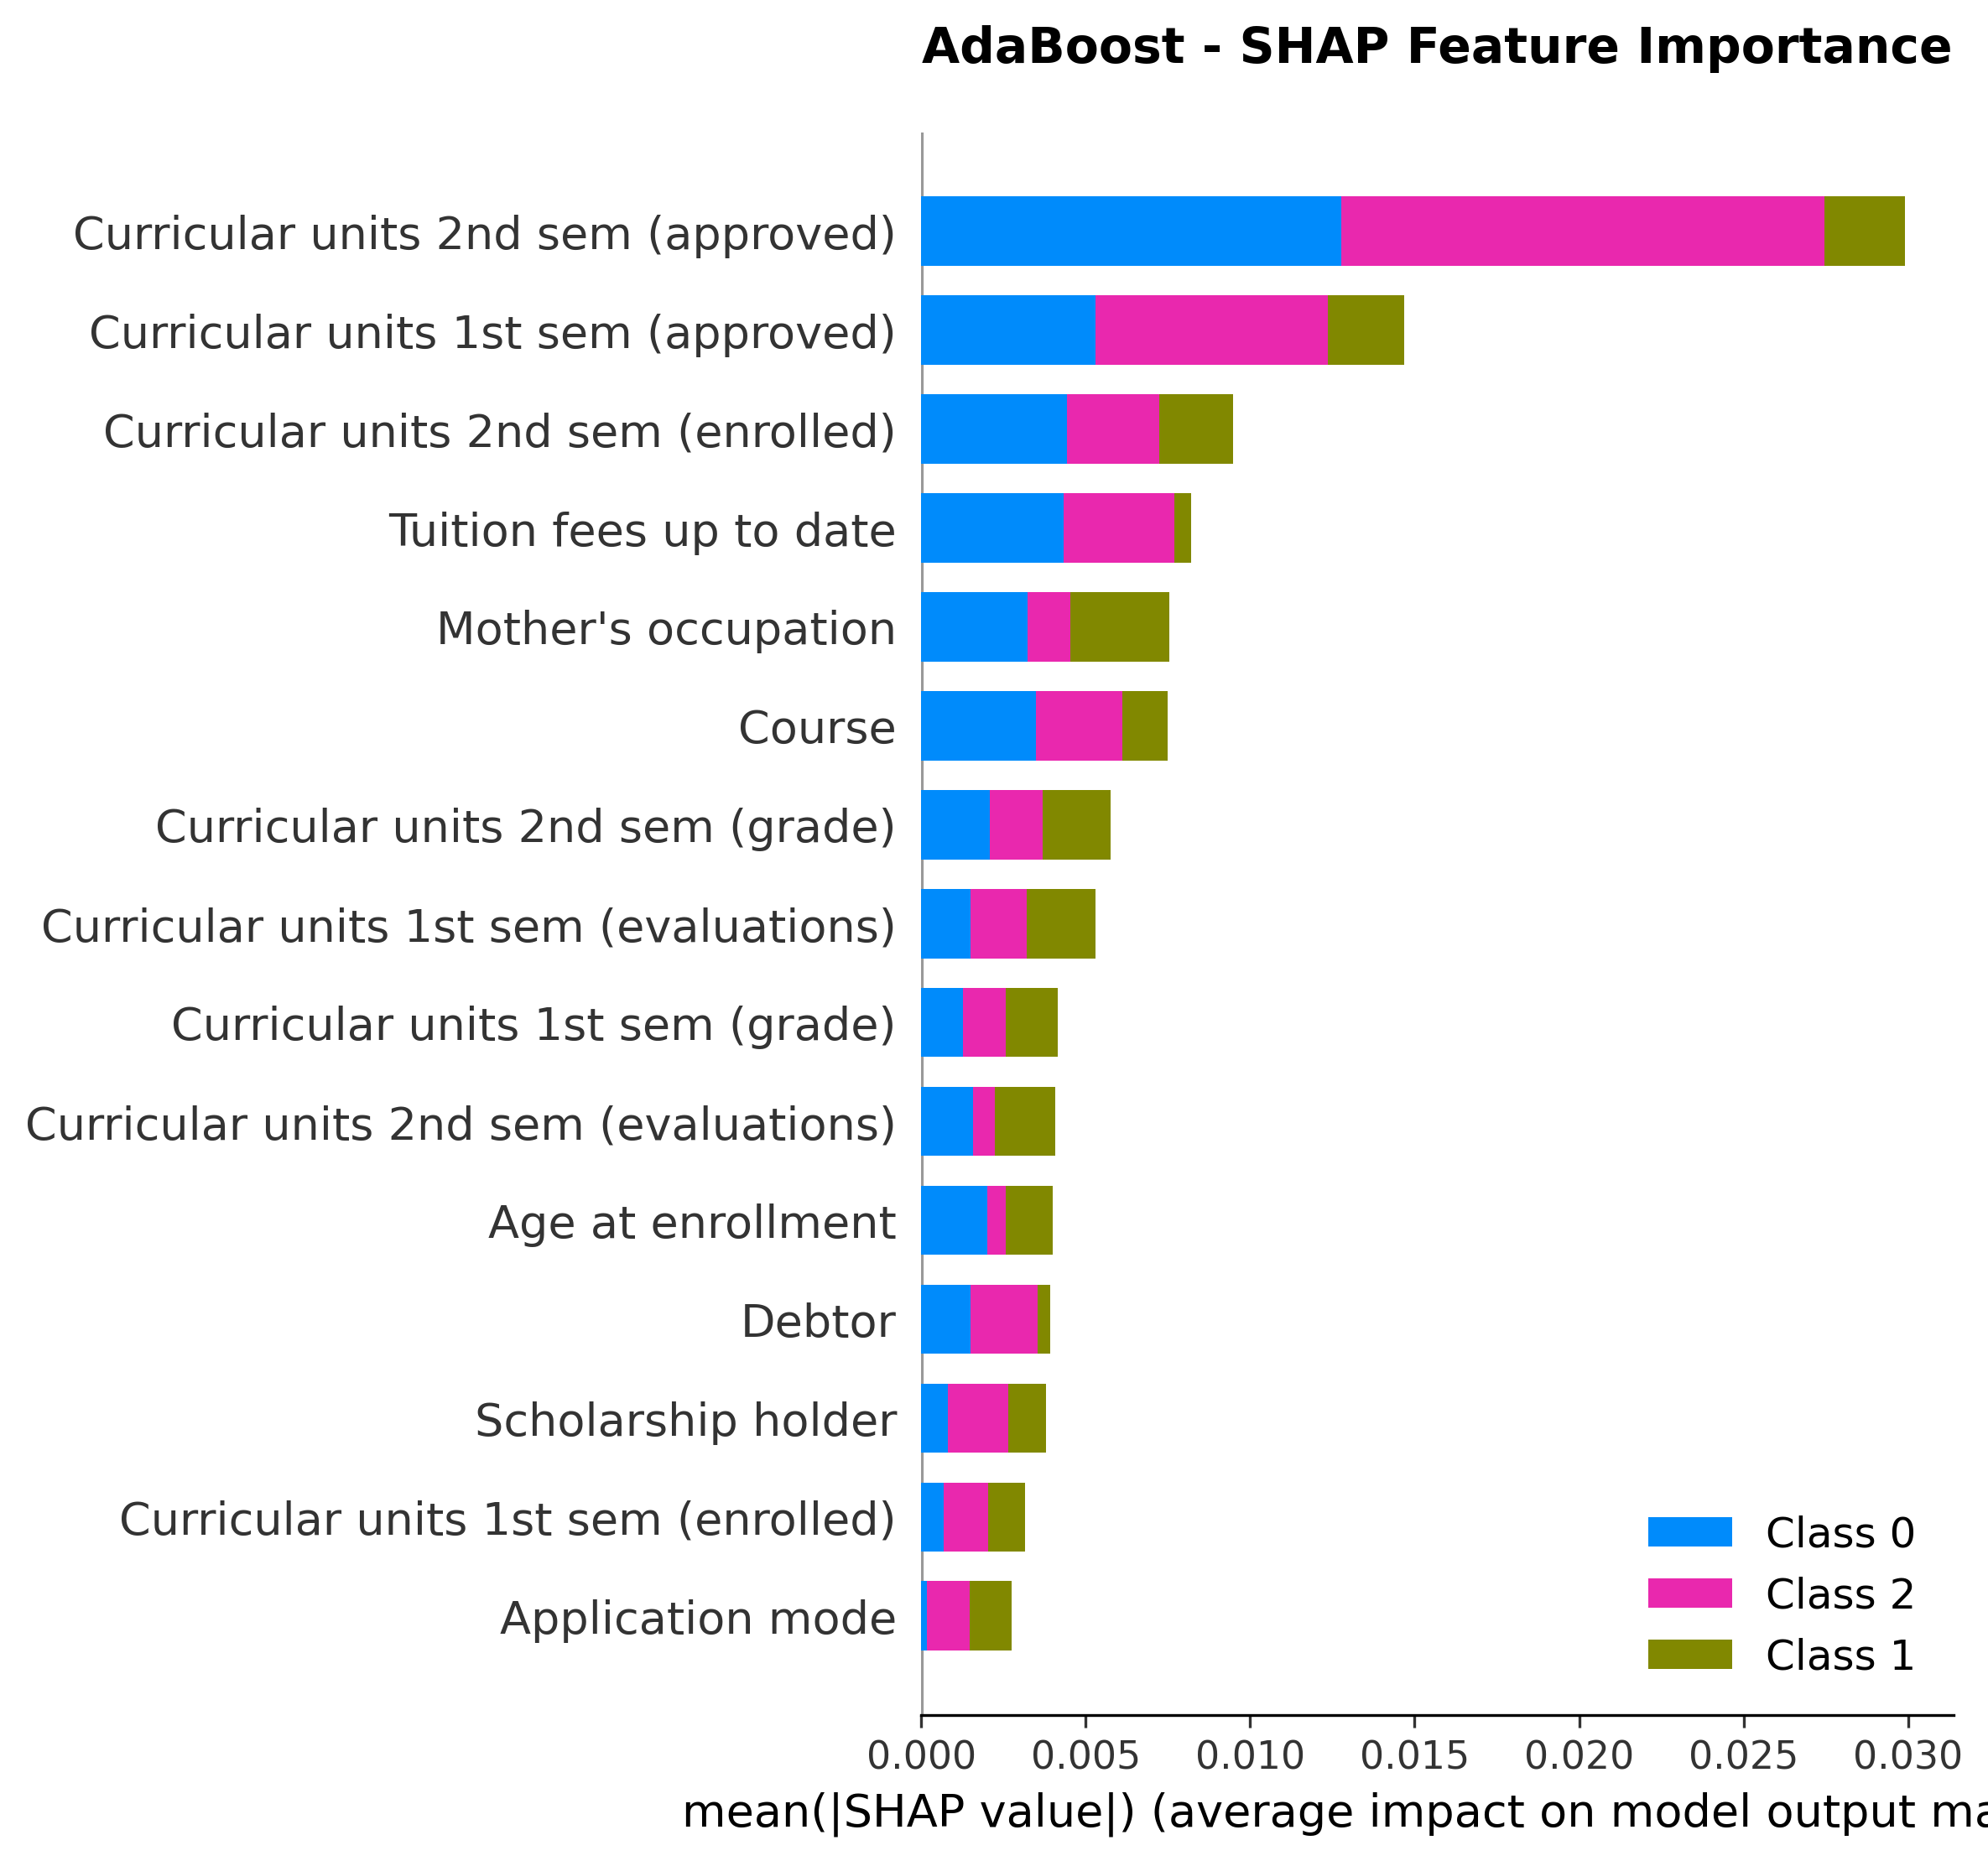
\includegraphics[width=0.85\textwidth]{supervisor_requirements/outputs/figures/11_shap_adaboost_importance.png}
    \caption{SHAP feature importance for AdaBoost}
    \label{fig:shap_ada_importance}
\end{figure}

\begin{figure}[htbp]
    \centering
    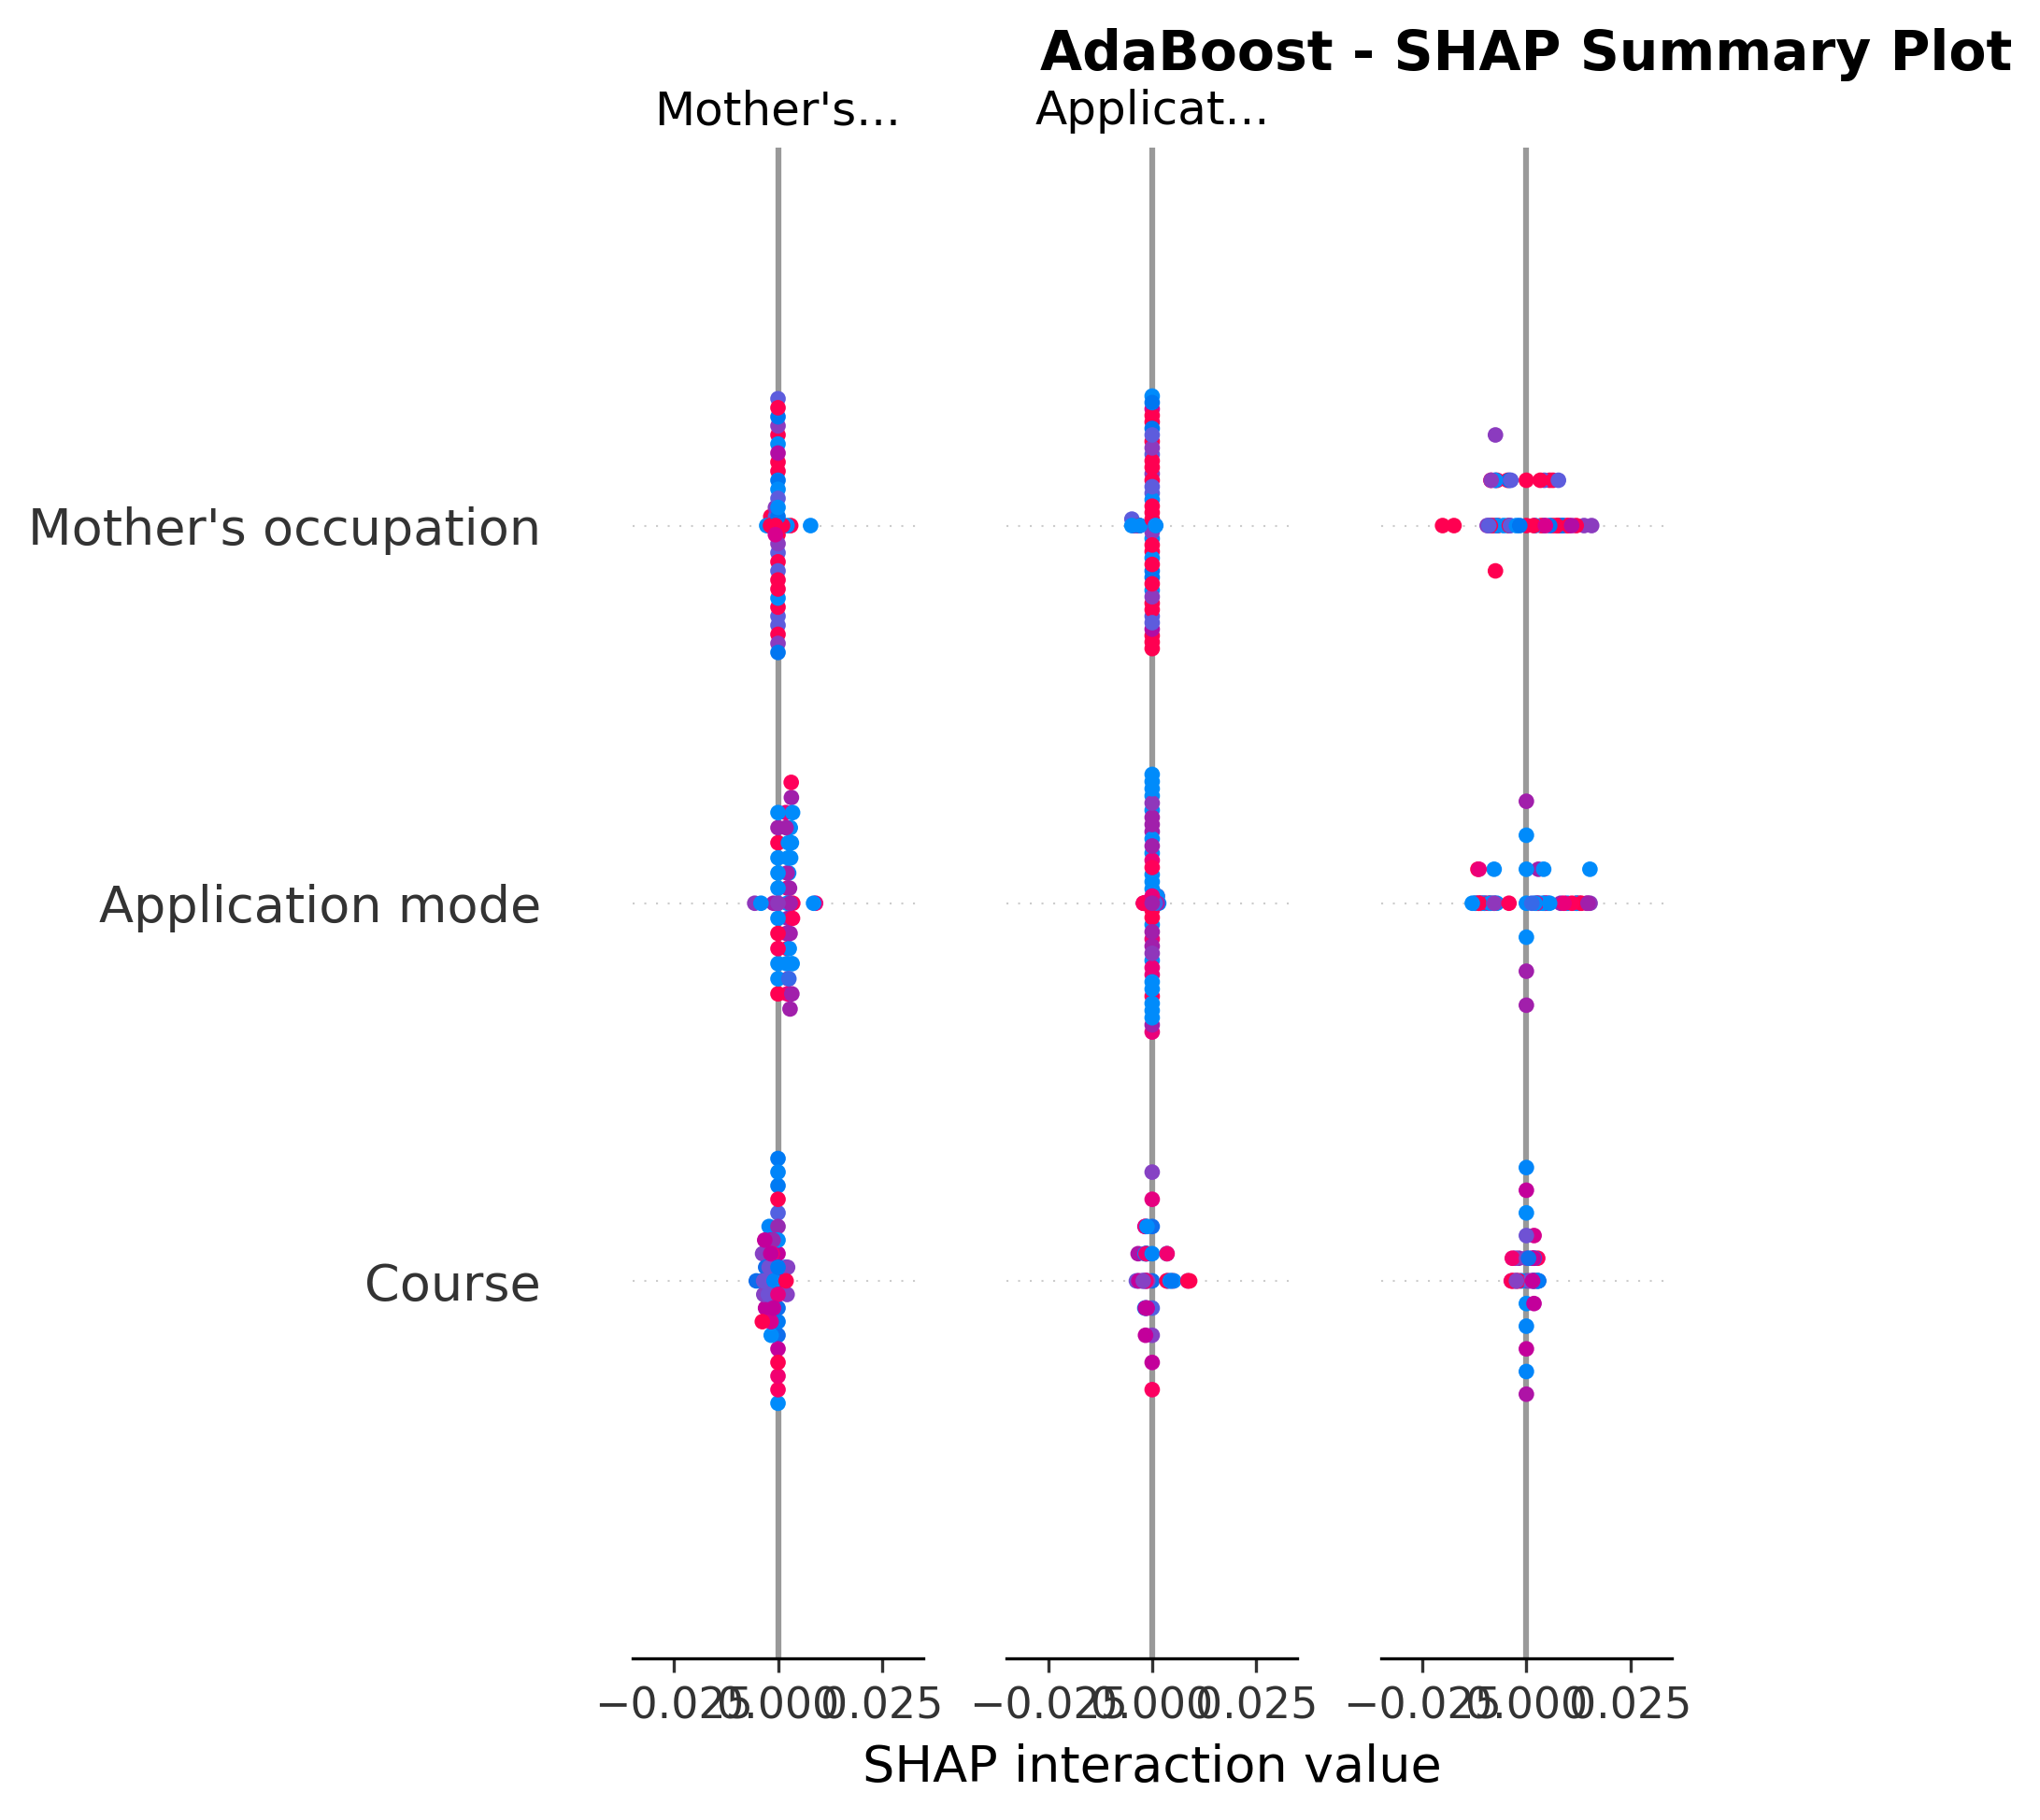
\includegraphics[width=0.85\textwidth]{supervisor_requirements/outputs/figures/11_shap_adaboost_summary.png}
    \caption{SHAP summary plot for AdaBoost}
    \label{fig:shap_ada_summary}
\end{figure}

\subsubsection{XGBoost}

\begin{figure}[htbp]
    \centering
    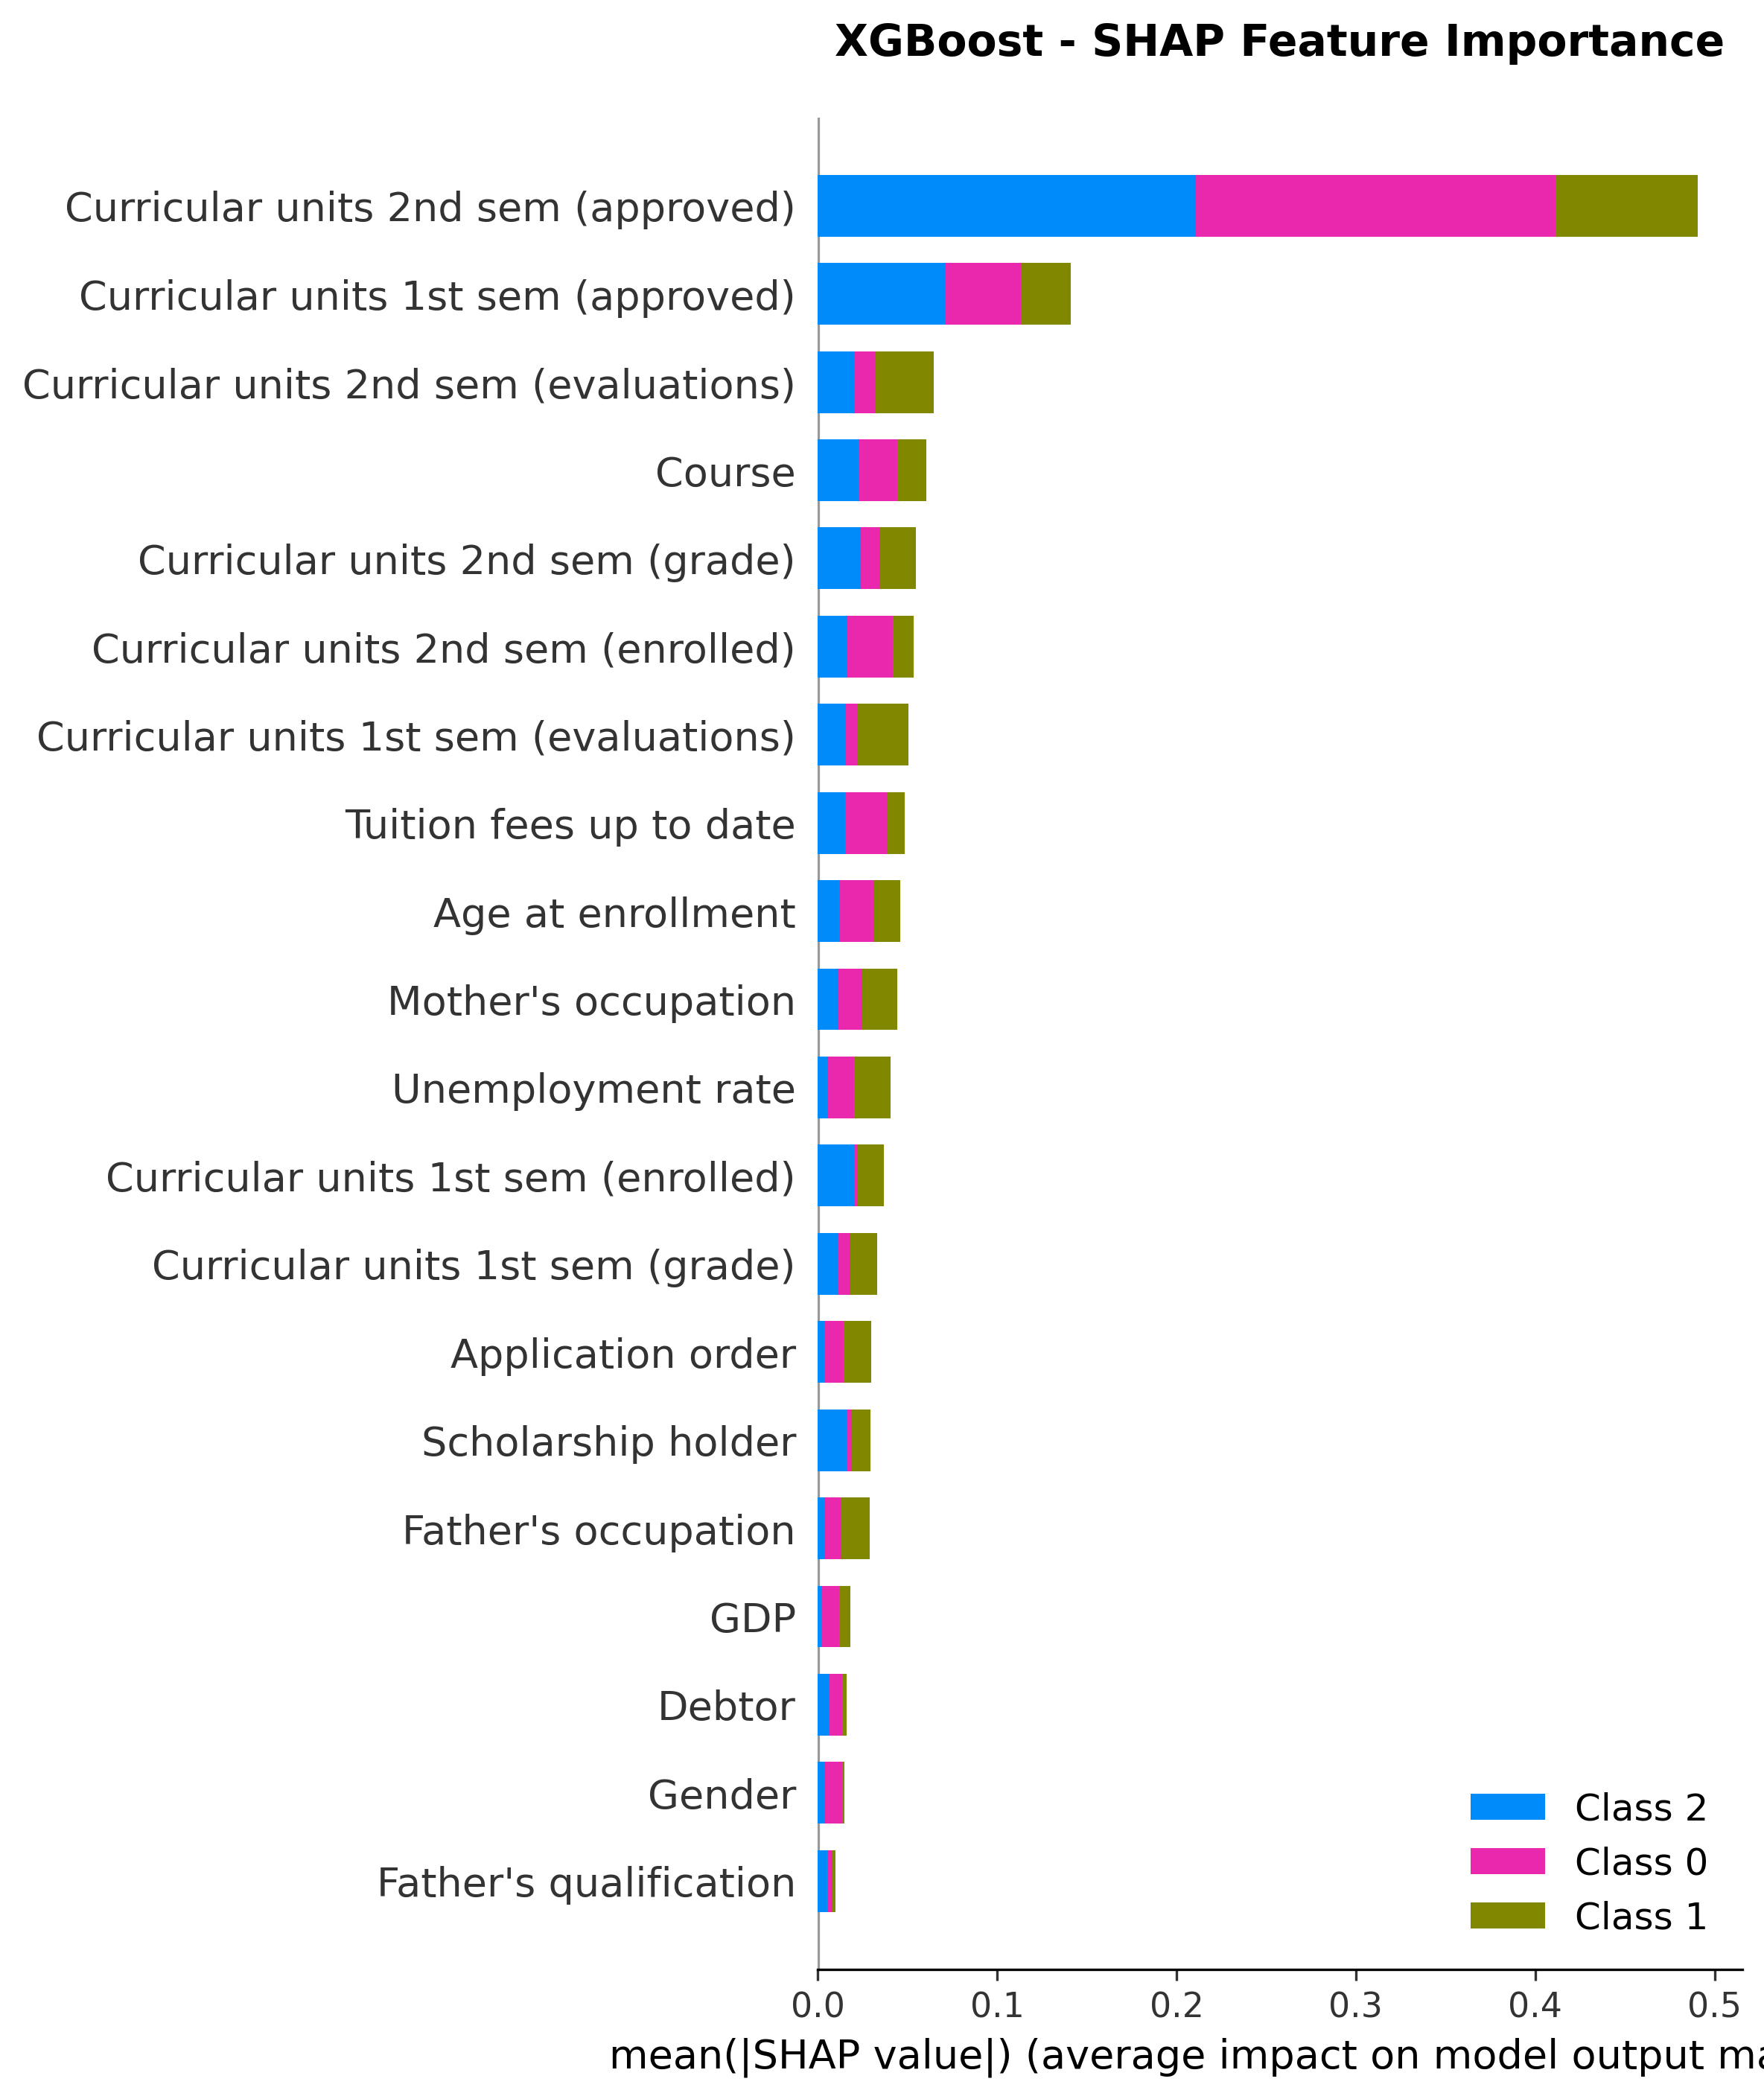
\includegraphics[width=0.85\textwidth]{supervisor_requirements/outputs/figures/11_shap_xgboost_importance.png}
    \caption{SHAP feature importance for XGBoost}
    \label{fig:shap_xgb_importance}
\end{figure}

\begin{figure}[htbp]
    \centering
    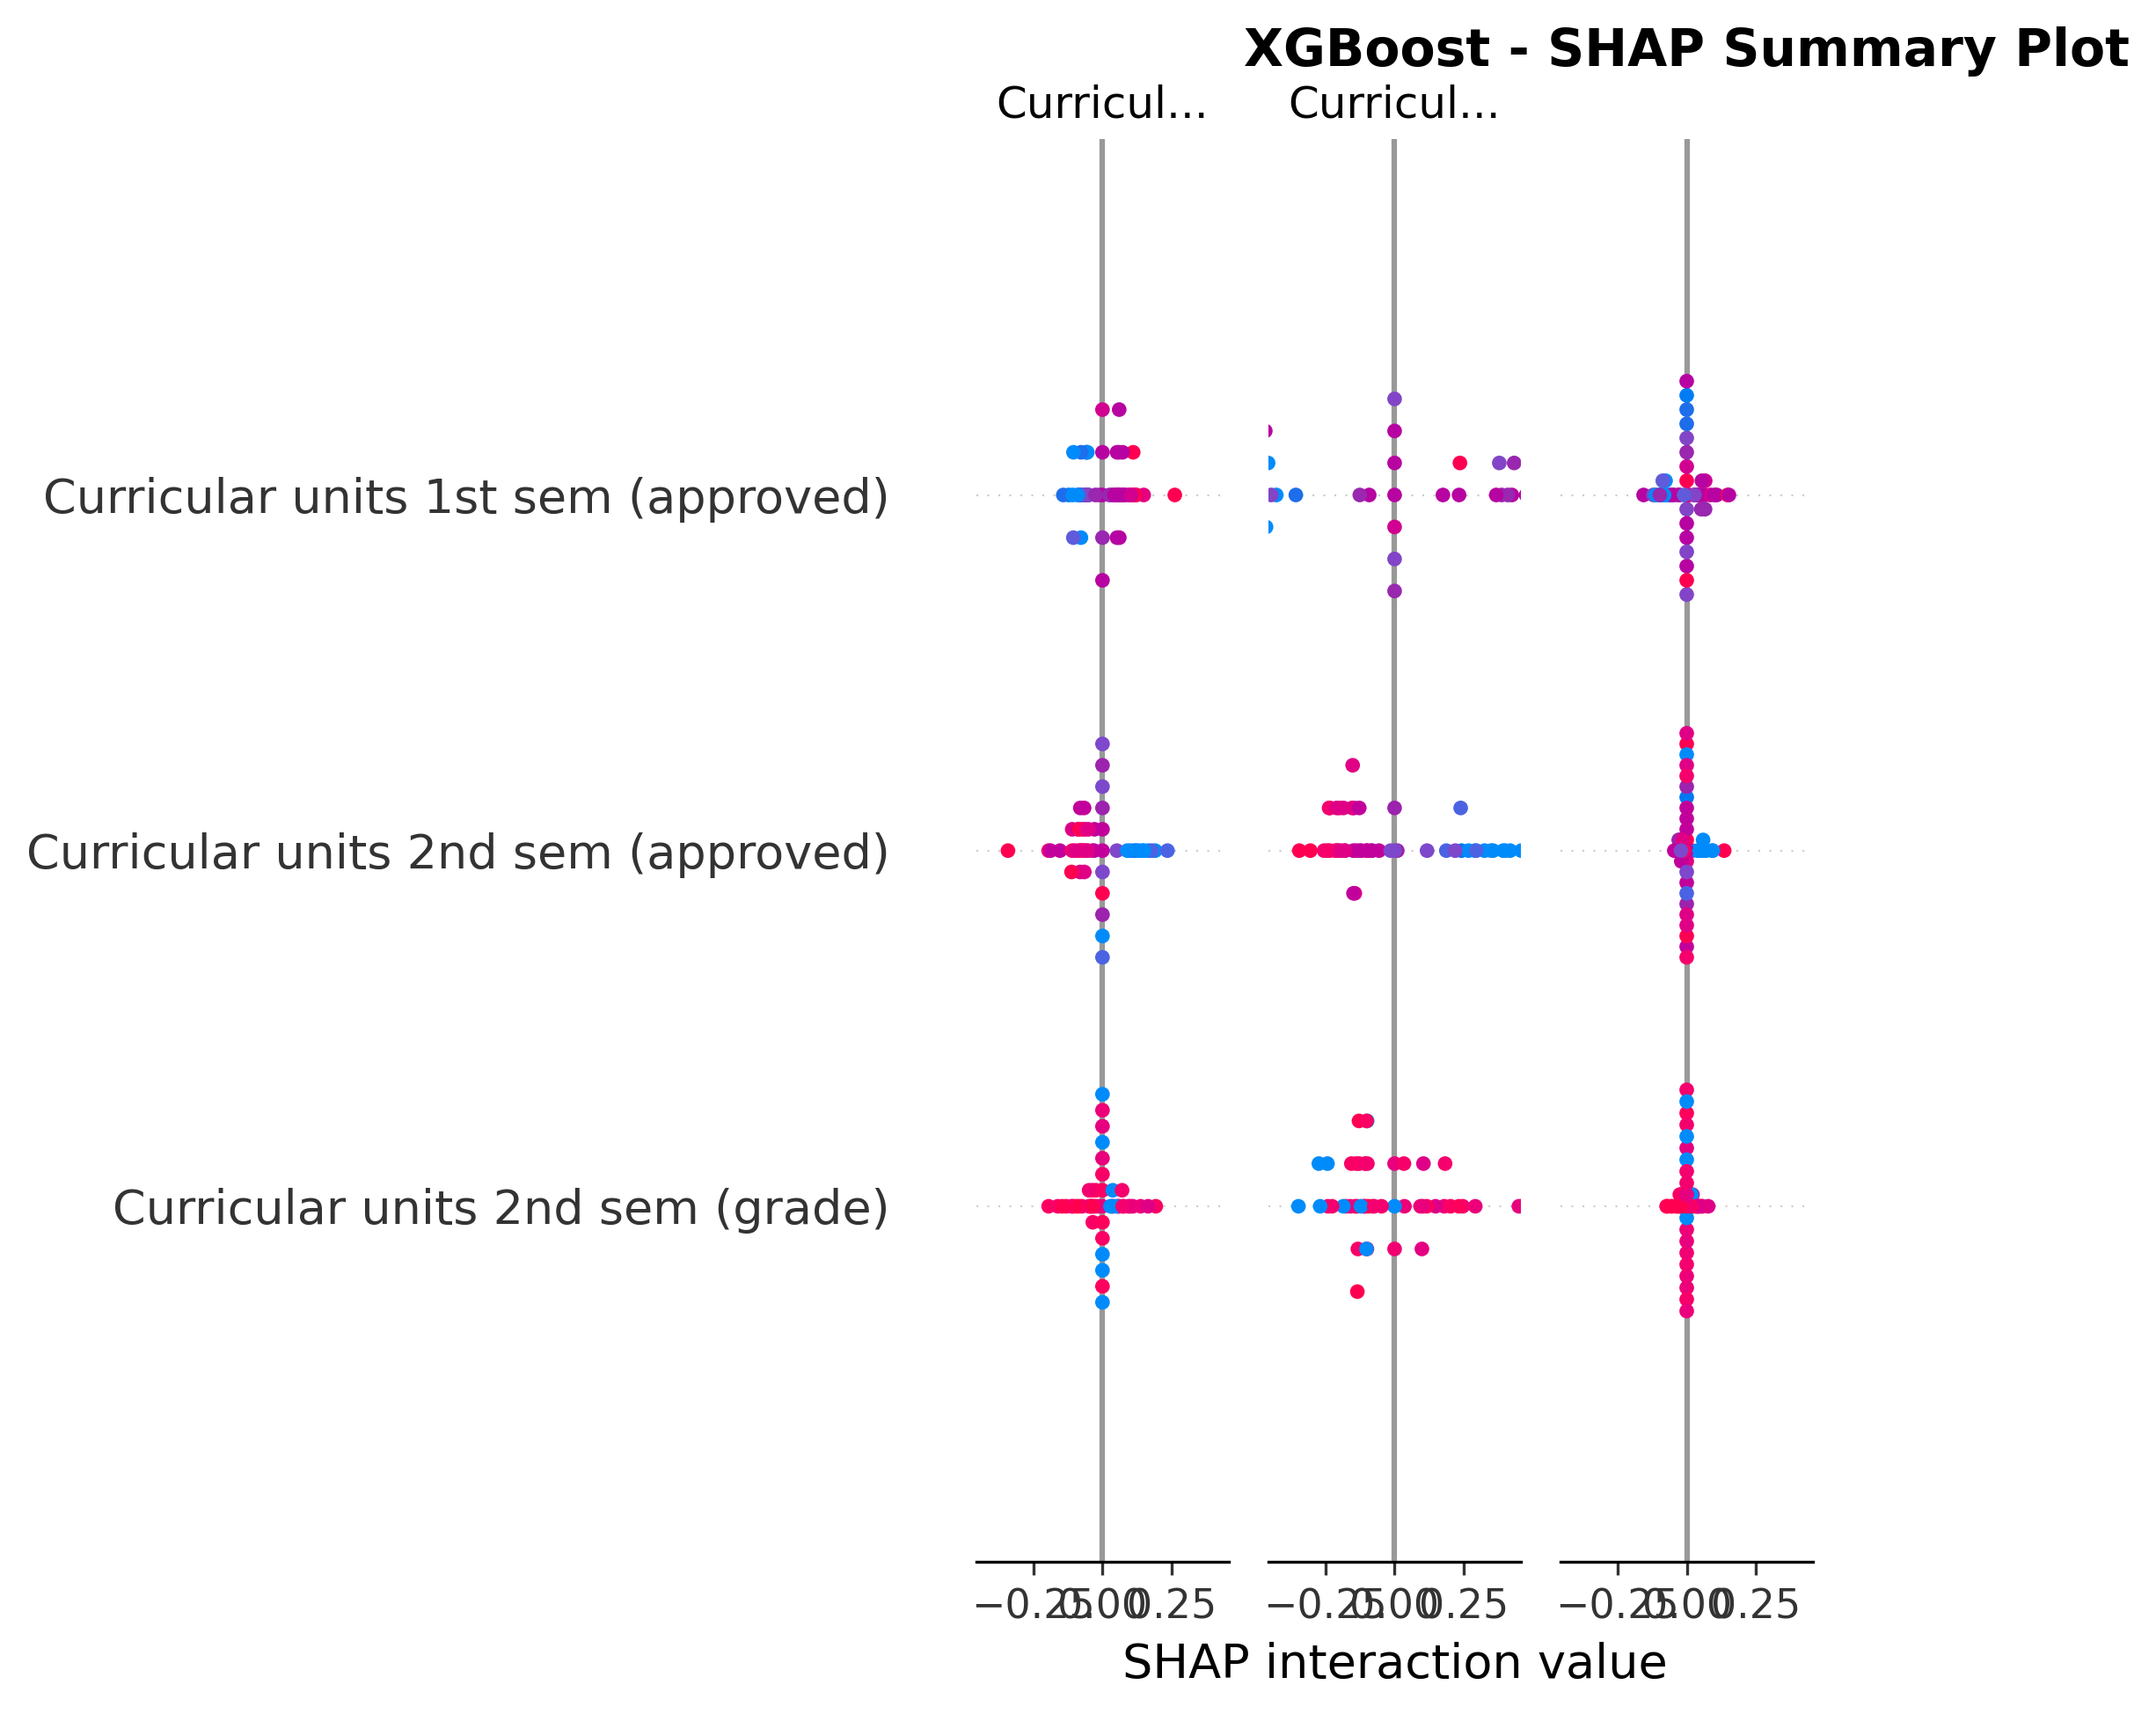
\includegraphics[width=0.85\textwidth]{supervisor_requirements/outputs/figures/11_shap_xgboost_summary.png}
    \caption{SHAP summary plot for XGBoost}
    \label{fig:shap_xgb_summary}
\end{figure}

\subsubsection{Neural Network}

\begin{figure}[htbp]
    \centering
    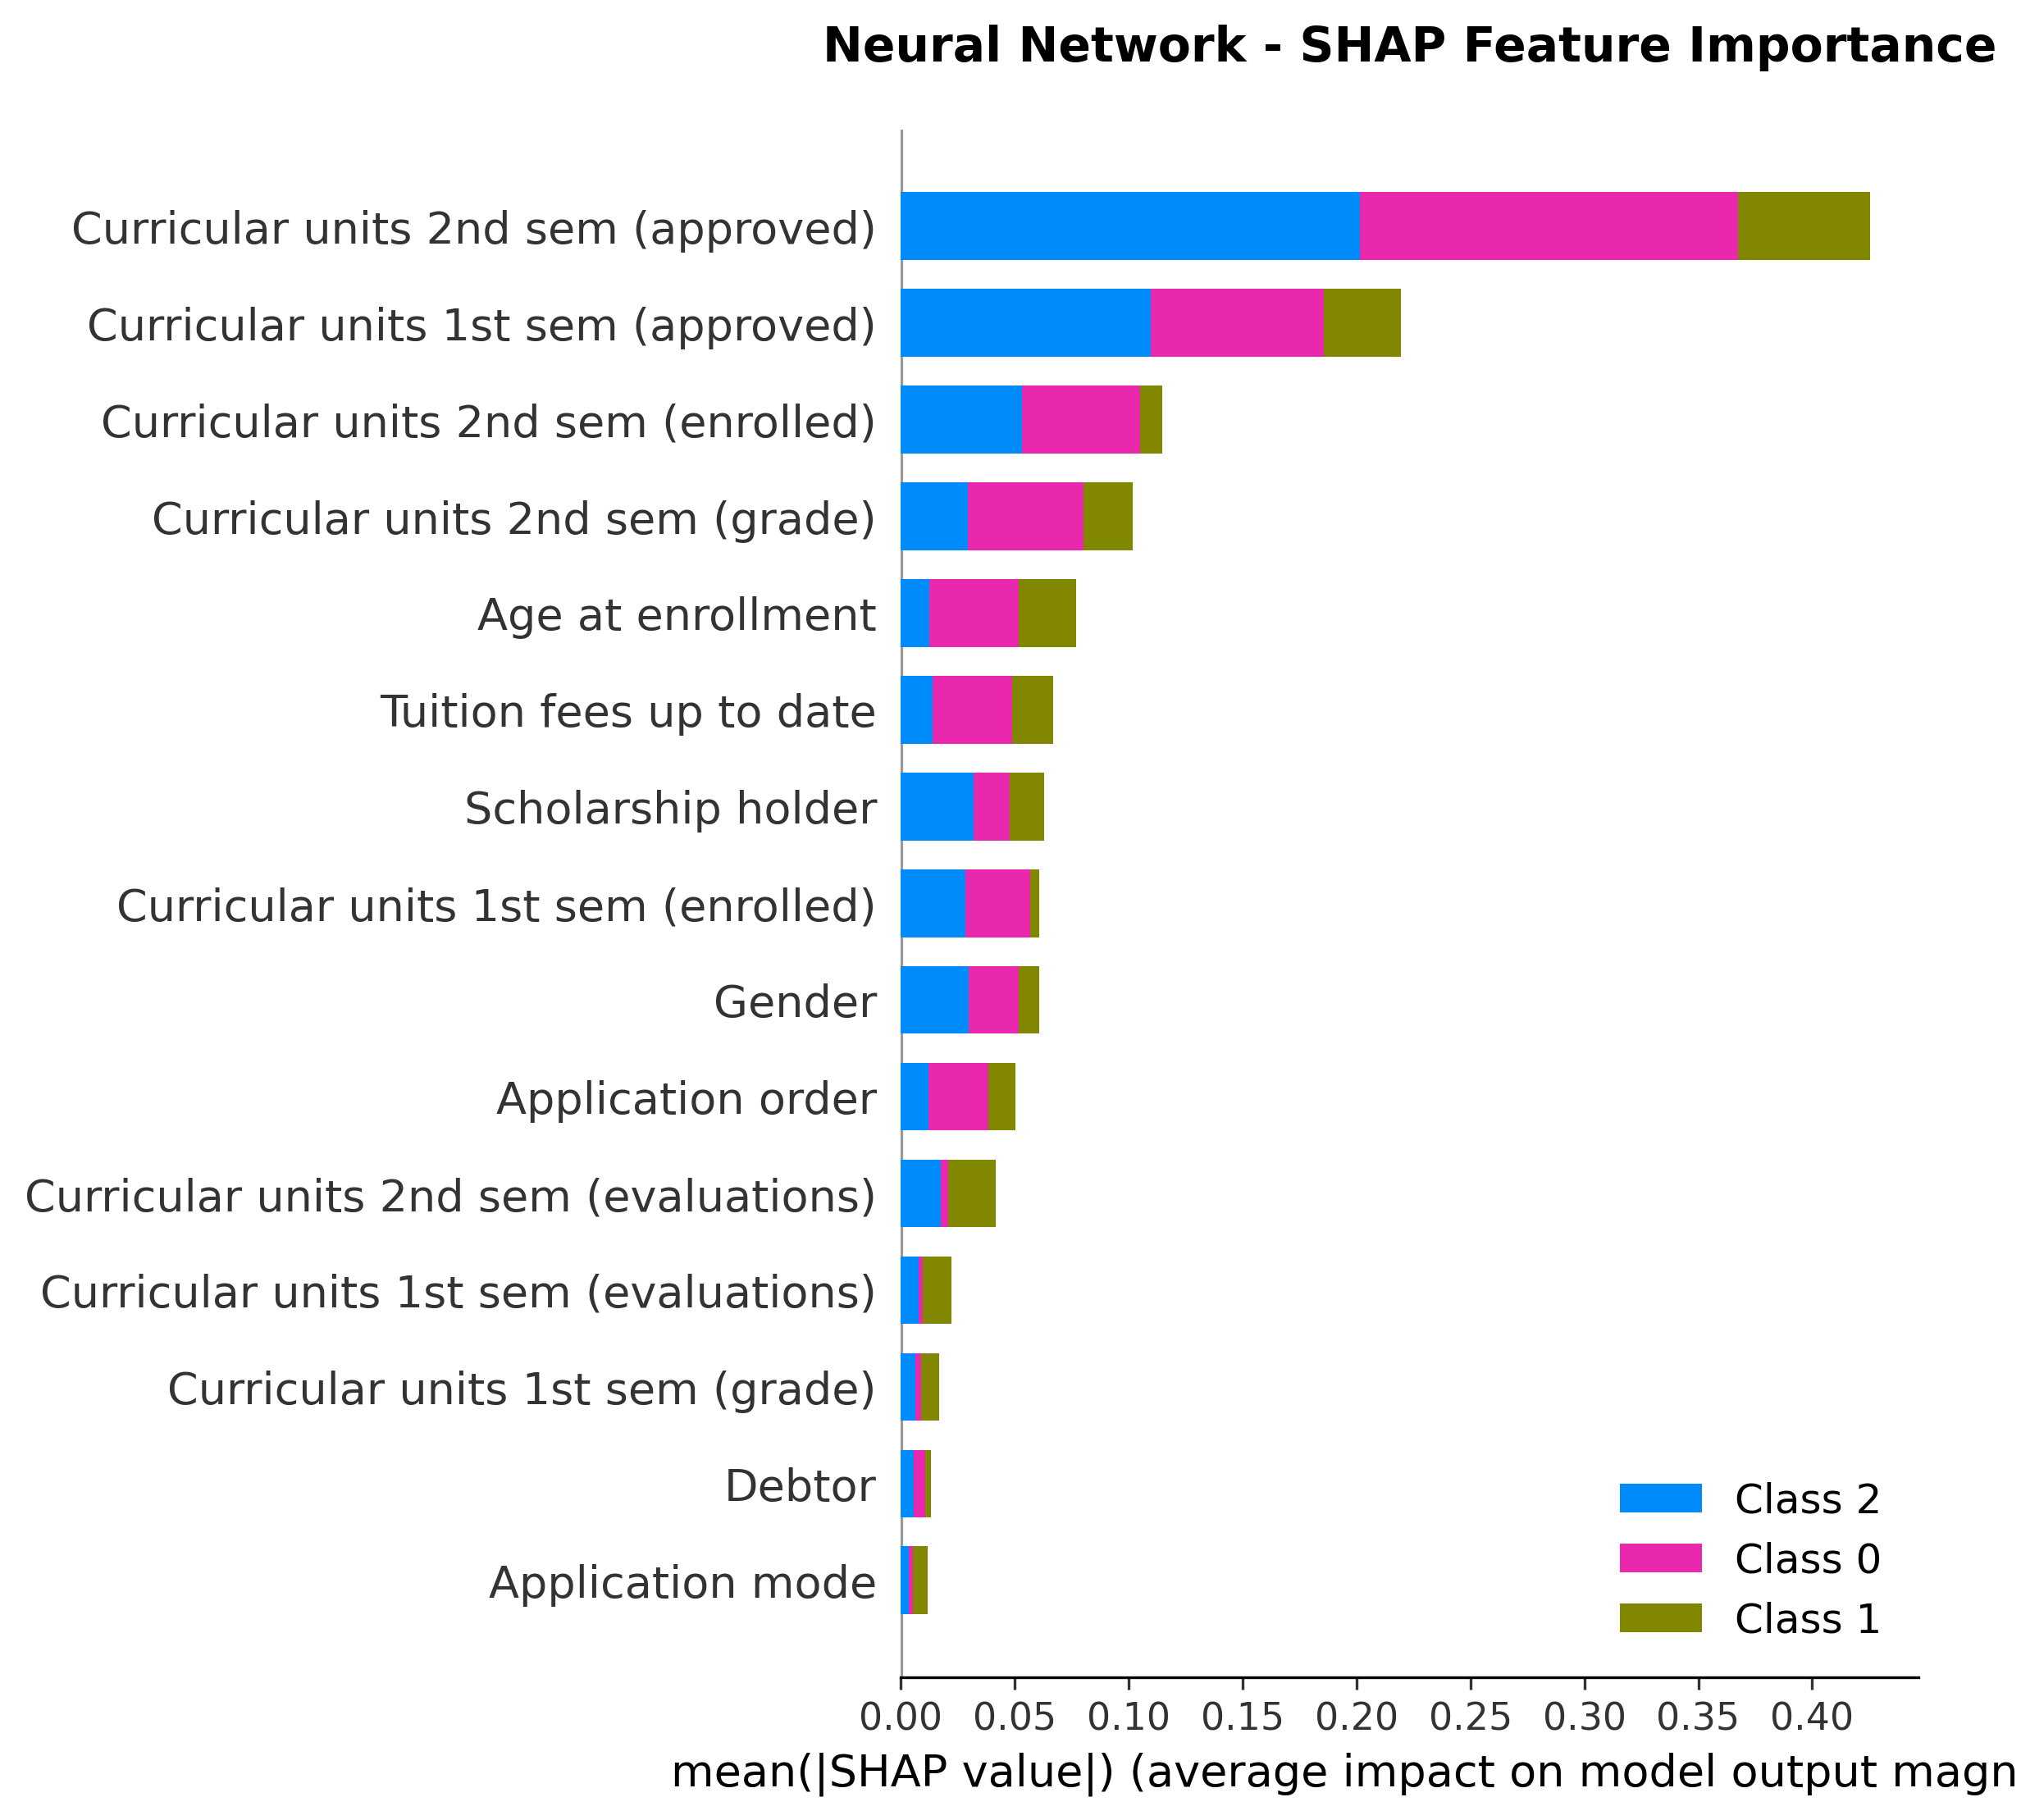
\includegraphics[width=0.85\textwidth]{supervisor_requirements/outputs/figures/11_shap_neural_network_importance.png}
    \caption{SHAP feature importance for Neural Network}
    \label{fig:shap_nn_importance}
\end{figure}

\begin{figure}[htbp]
    \centering
    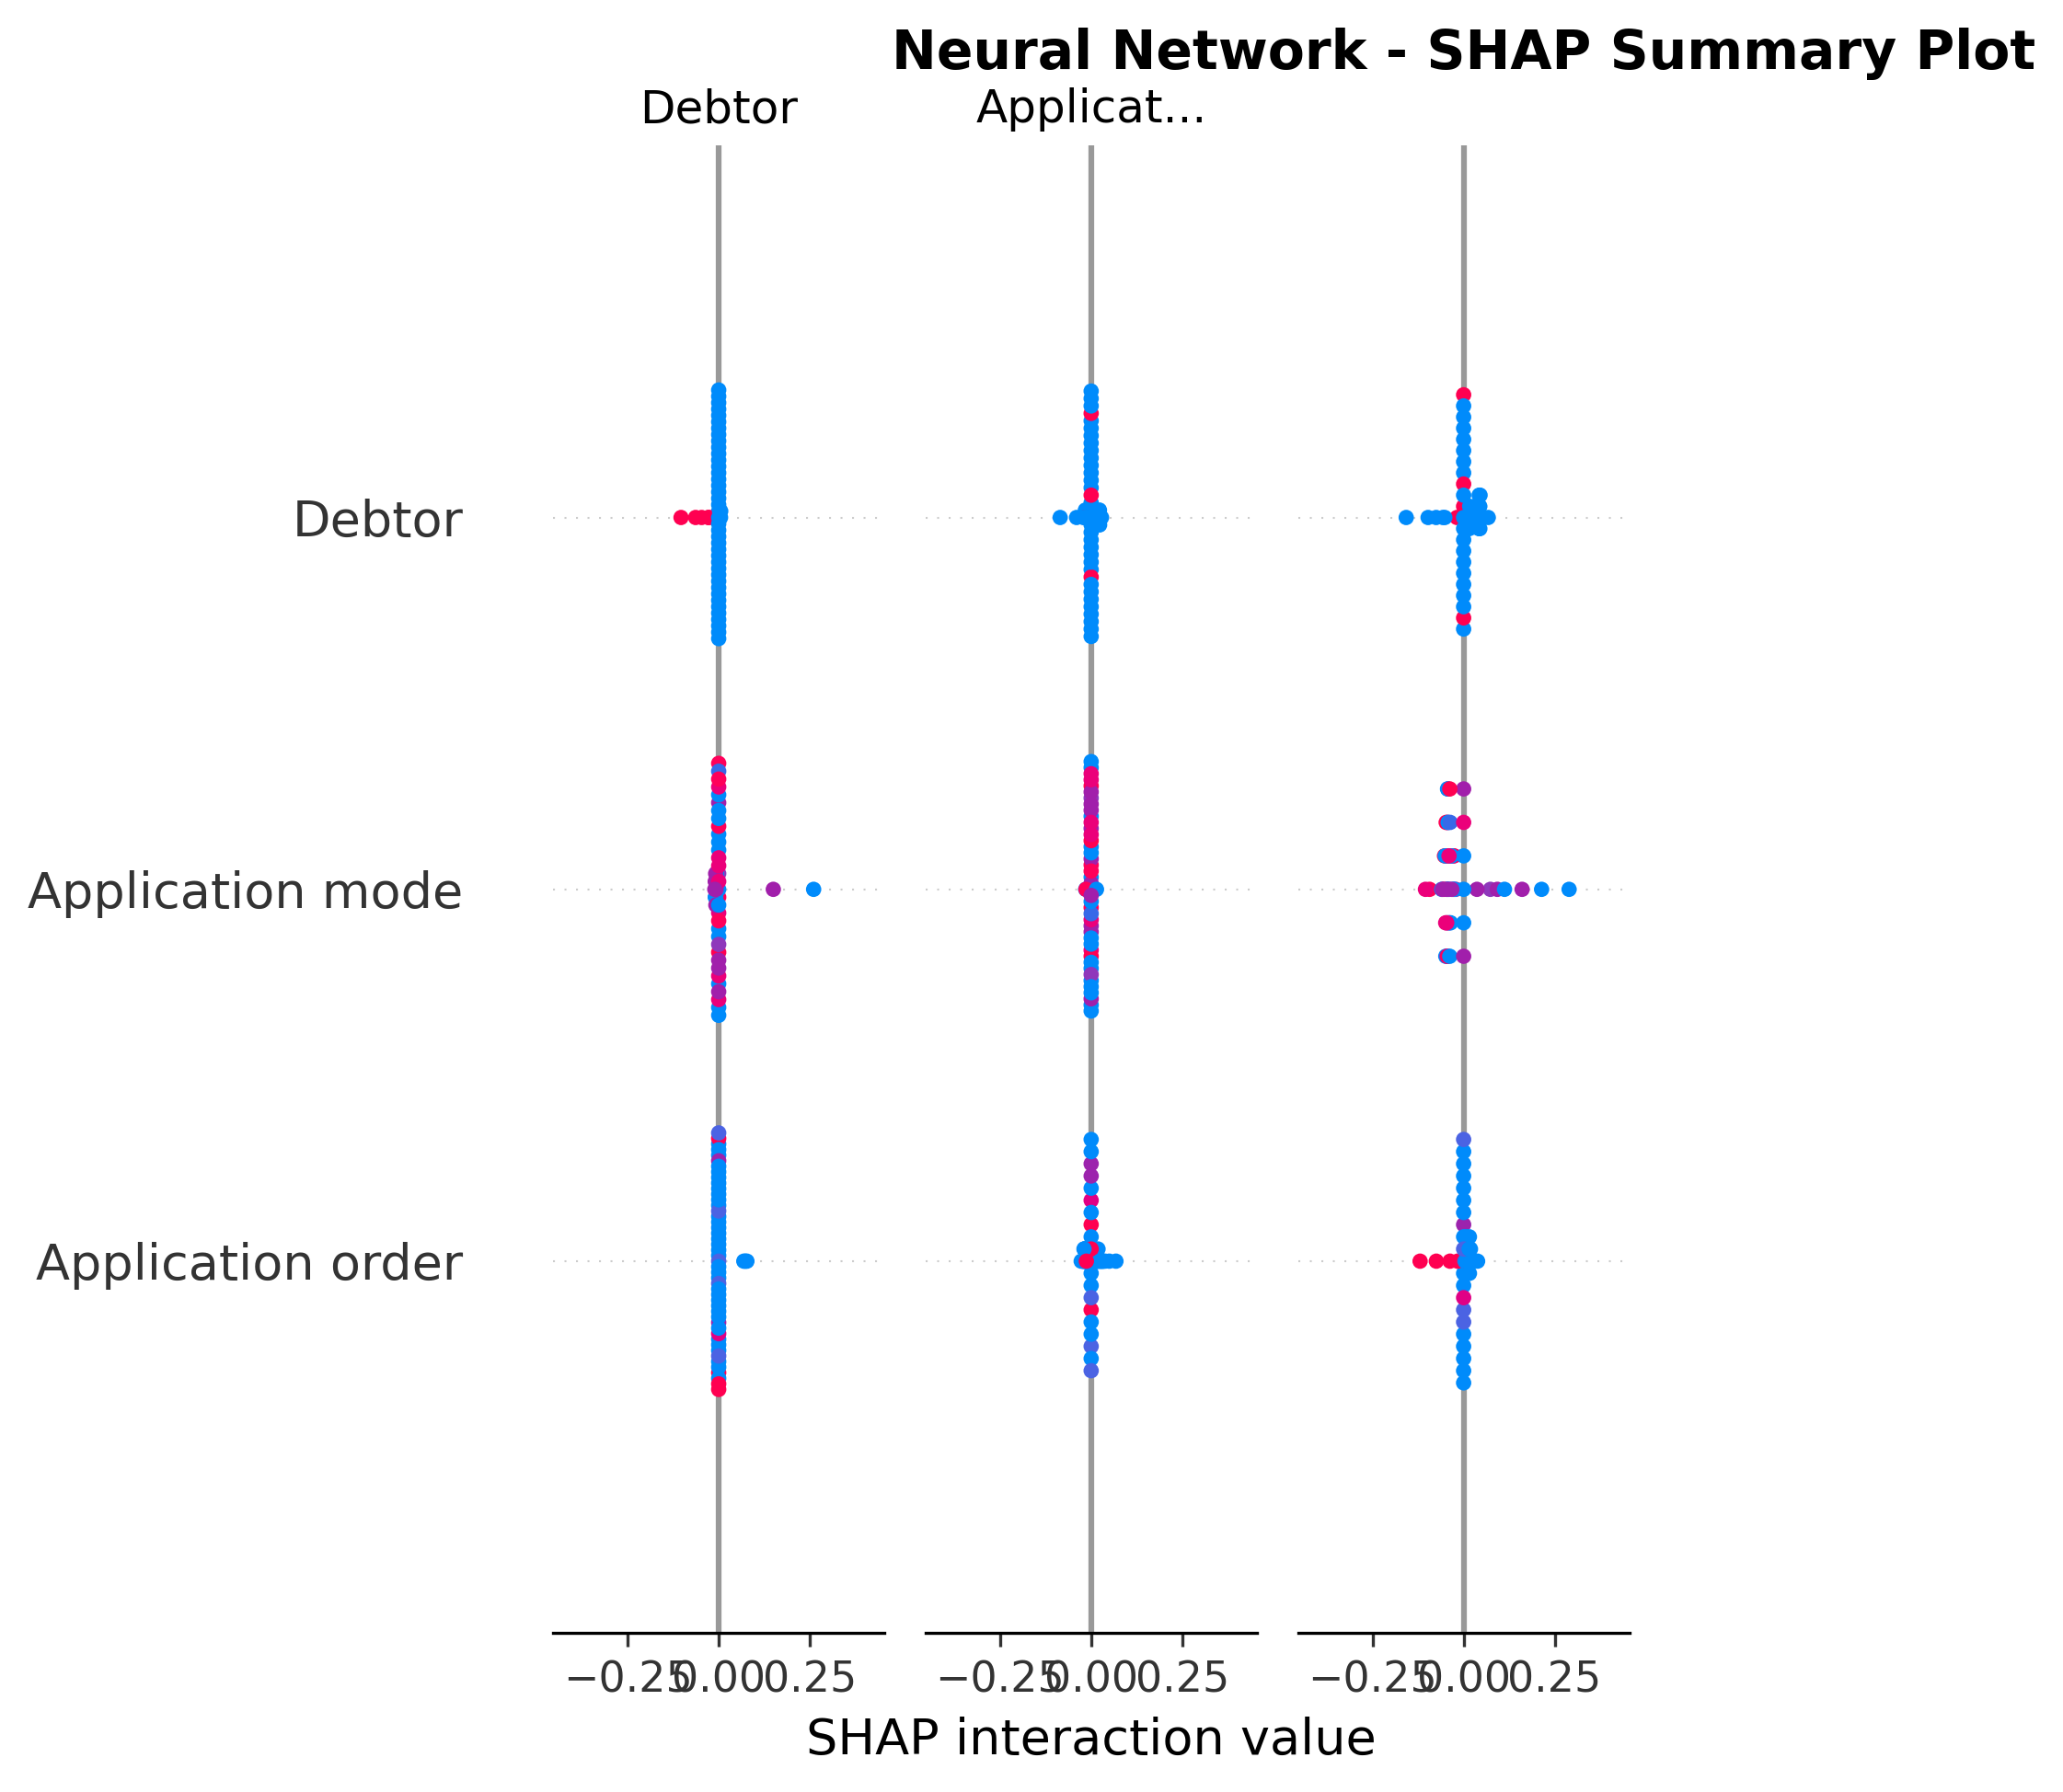
\includegraphics[width=0.85\textwidth]{supervisor_requirements/outputs/figures/11_shap_neural_network_summary.png}
    \caption{SHAP summary plot for Neural Network}
    \label{fig:shap_nn_summary}
\end{figure}

\subsection{Cross-Model SHAP Insights}

\begin{figure}[htbp]
    \centering
    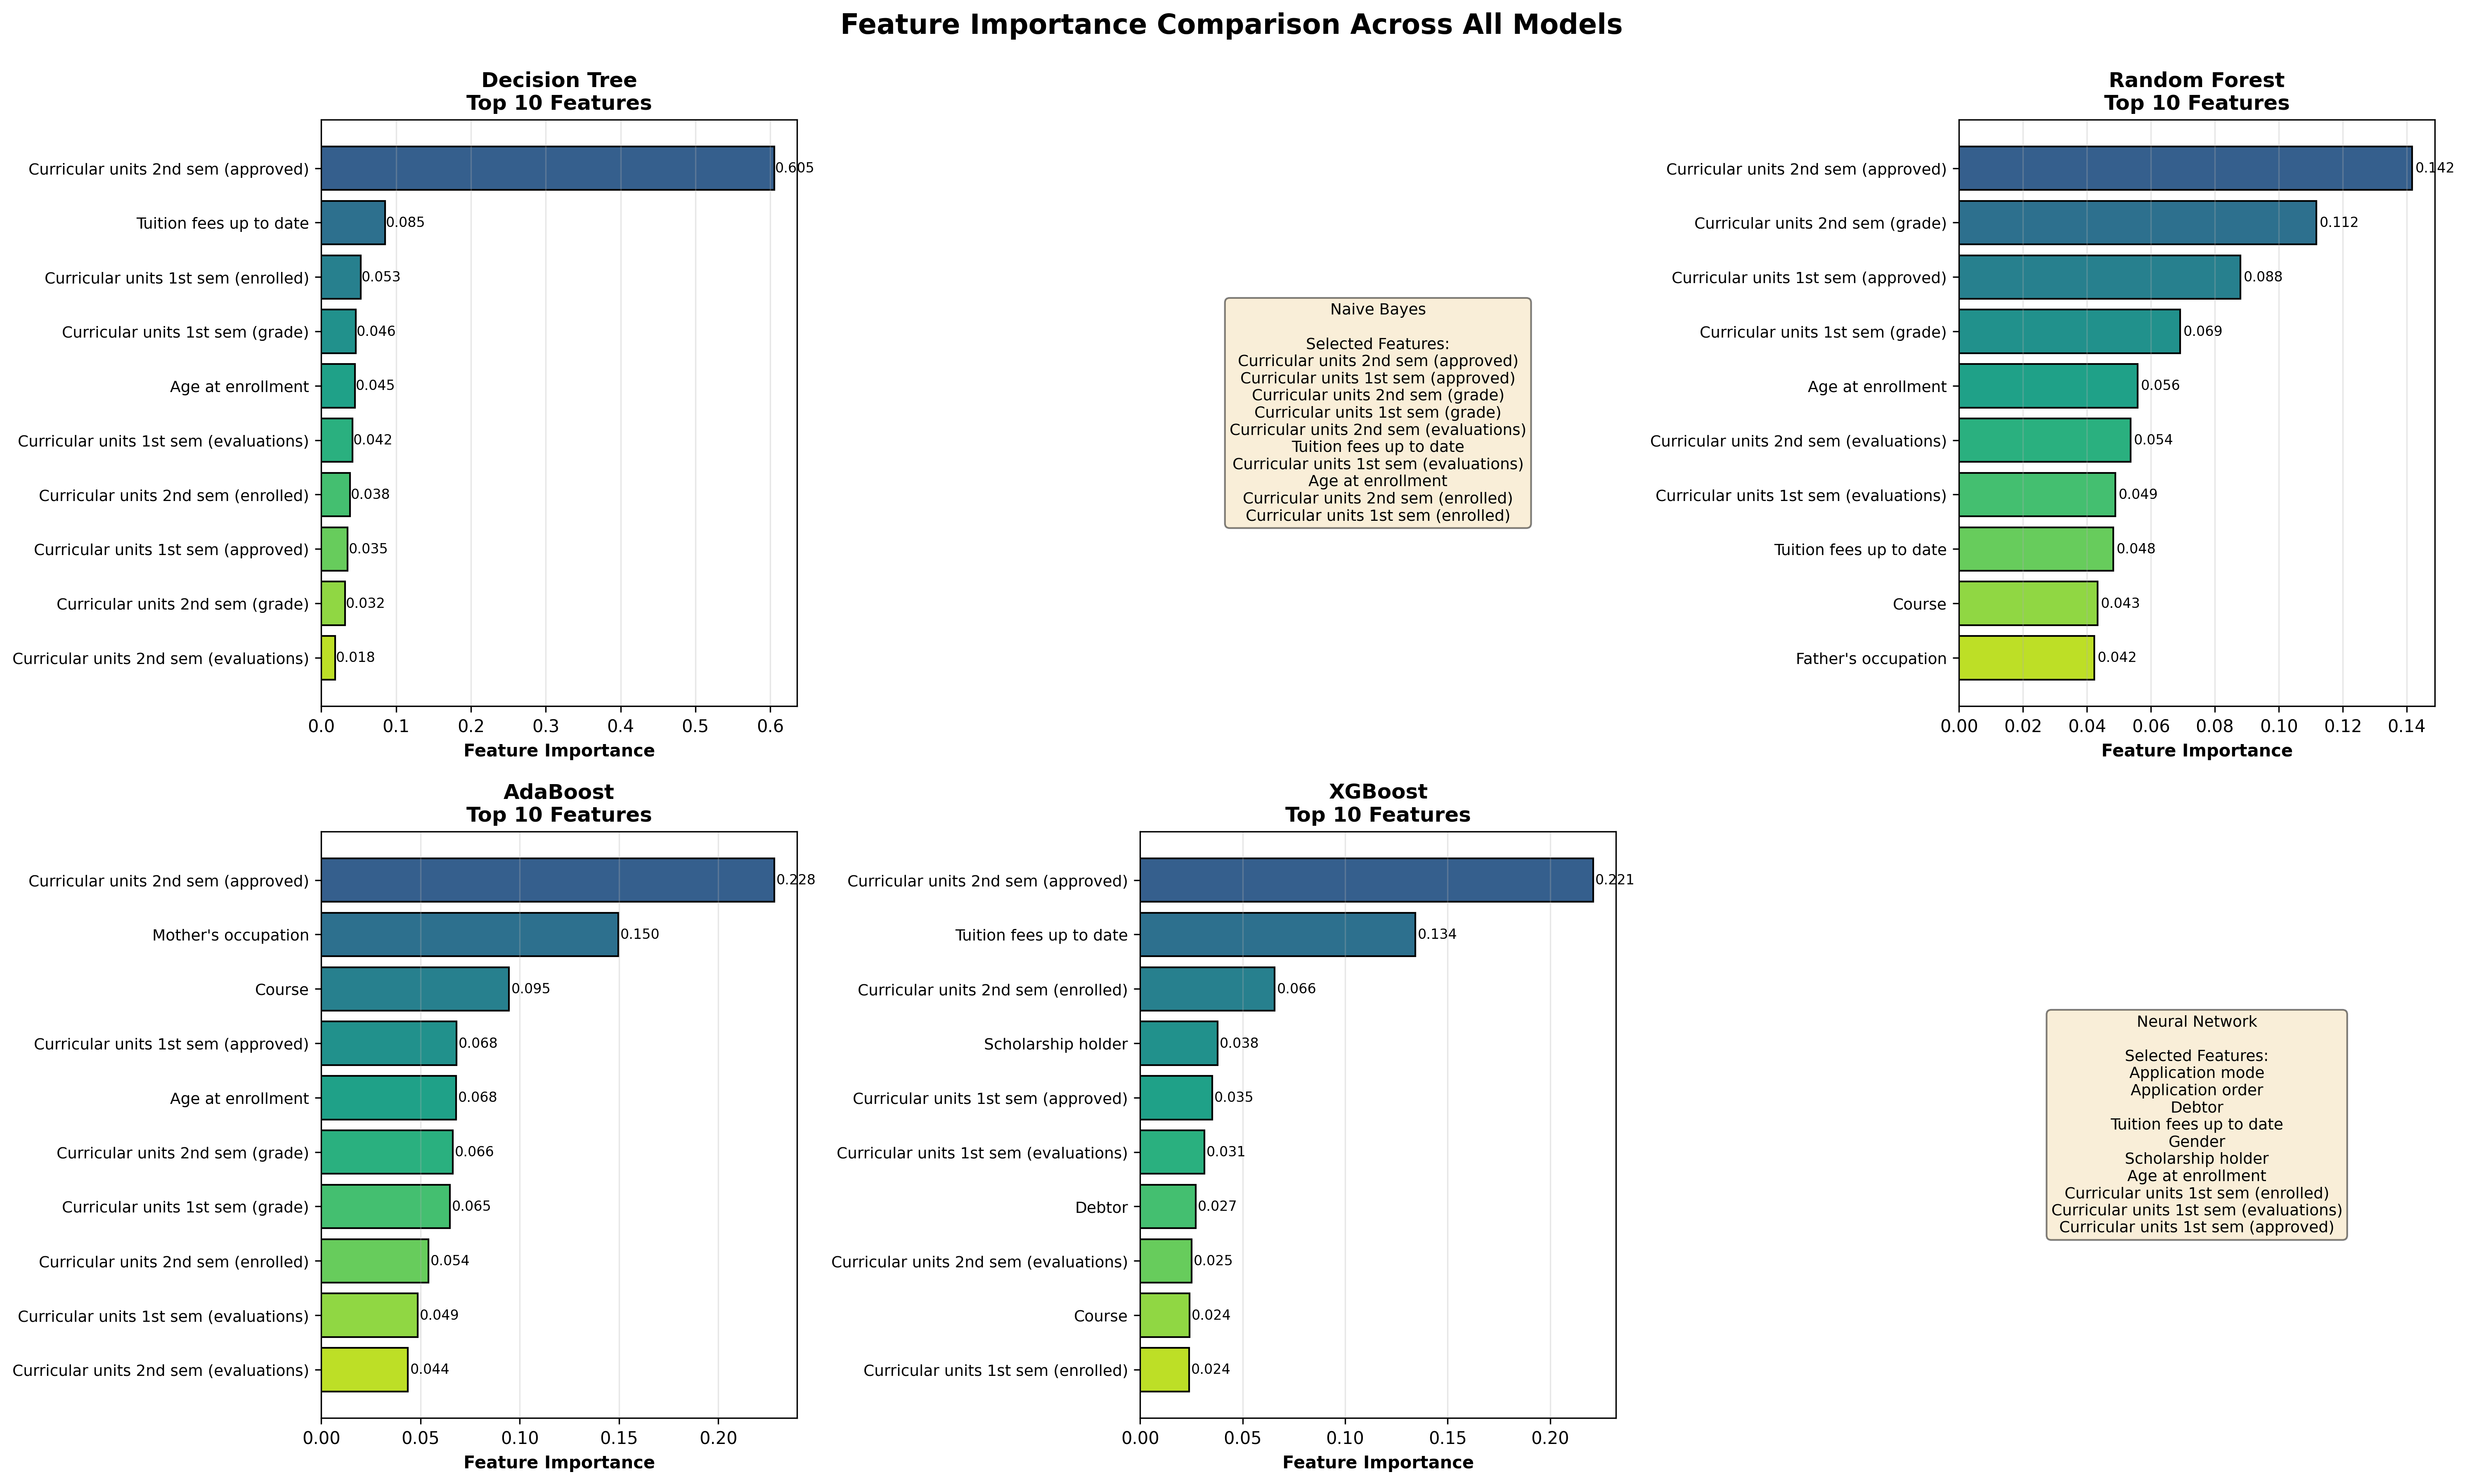
\includegraphics[width=\textwidth]{supervisor_requirements/outputs/figures/11_all_models_feature_importance_comparison.png}
    \caption{Feature importance comparison across all models using SHAP}
    \label{fig:shap_comparison}
\end{figure}

\textbf{Key Findings}:
\begin{itemize}
    \item Curricular units (approved and grades) consistently ranked highest across all models
    \item Tuition fee status and scholarship holder appeared in top 10 for all models
    \item SHAP rankings aligned closely with statistical feature ranking methods
    \item Age showed non-linear effects with both very young and older students having different risk profiles
\end{itemize}

\section{Discussion}
\label{sec:discussion}

\subsection{Feature Importance Consensus}

Statistical ranking and SHAP analysis converged on key findings:
\begin{enumerate}
    \item \textbf{Academic performance dominates}: Curricular units (approved, grades) strongest predictors
    \item \textbf{Temporal progression matters}: Second semester metrics slightly more important
    \item \textbf{Financial stability critical}: Tuition payment and scholarship receipt top-tier features
    \item \textbf{Early warning capability}: First semester performance enables early intervention
\end{enumerate}

\subsection{Model Performance Hierarchy}

\textbf{Ensemble Superiority}:
\begin{itemize}
    \item 7-11 percentage points higher accuracy than Decision Tree
    \item 9-15\% AUC improvement over baseline classifiers
    \item Lower cross-validation variance
\end{itemize}

\textbf{Random Forest vs XGBoost}:
\begin{itemize}
    \item XGBoost: Higher CV accuracy (78.21\%)
    \item Random Forest: Lower overfitting (12.45\% vs 21.07\%), better calibration
    \item Random Forest recommended for deployment
\end{itemize}

\subsection{Class-Specific Patterns}

\textbf{Graduate Class}: 92\% recall - strong identification of successful students

\textbf{Dropout Class}: 74\% recall - moderate success with room for improvement

\textbf{Enrolled Class}: 39\% recall - inherent difficulty due to transitional state

\subsection{Practical Implications}

\textbf{Early Warning System}:
\begin{itemize}
    \item Deploy at end of first semester
    \item Identify students with < 50\% course approval
    \item Flag financial warning signs
\end{itemize}

\textbf{Targeted Interventions}:
\begin{itemize}
    \item Academic struggles: Tutoring, study skills workshops
    \item Financial difficulties: Emergency loans, payment plans
    \item Combined risk: Comprehensive support packages
\end{itemize}

\subsection{Limitations}

\textbf{Data Limitations}:
\begin{itemize}
    \item Single-institution snapshot
    \item Missing psychological, social, health factors
    \item Historical data may not reflect current programs
\end{itemize}

\textbf{Model Limitations}:
\begin{itemize}
    \item Ensemble methods lack full transparency despite SHAP
    \item Potential fairness concerns
    \item Performance may degrade as populations evolve
\end{itemize}

\subsection{Future Directions}

\begin{enumerate}
    \item Longitudinal studies tracking students over multiple years
    \item Randomized controlled trials measuring intervention effectiveness
    \item Multimodal data incorporating LMS logs, library usage, campus engagement
    \item Transfer learning across institutions
    \item Fairness-aware models optimizing for equity
    \item Causal inference identifying intervention targets
\end{enumerate}

\subsection{Contributions}

\begin{enumerate}
    \item Comprehensive evaluation framework combining multiple feature ranking with explainable AI
    \item Systematic multi-model comparison for evidence-based selection
    \item Focus on readily available institutional data
    \item Integration of interpretability (SHAP) for trustworthy educational AI
\end{enumerate}

\section{Summary}

The experimental results validate machine learning effectiveness for student dropout prediction:

\textbf{Best Performance}:
\begin{itemize}
    \item Random Forest: 76.72\% accuracy, 0.9062 AUC
    \item XGBoost: 78.21\% CV accuracy, 0.9057 AUC
\end{itemize}

\textbf{Key Findings}:
\begin{itemize}
    \item Academic performance (approved courses, grades) = strongest predictors
    \item Financial stability indicators provide crucial complementary signals
    \item Ensemble methods significantly outperform single classifiers
    \item SHAP analysis enables interpretable predictions for high-stakes decisions
\end{itemize}

These findings enable evidence-based early warning systems identifying at-risk students with sufficient accuracy to guide targeted interventions, combining predictive performance with interpretability to support effective and ethical machine learning in education.
